%Começa na imagem 26.jpg
\chapter{1. Tempo e espaço: fontes e formas de representação}

%Orientações para o professor:

\coment{Habilidades da BNCC envolvidas:

EF05HI0: Identificar os processos de formação das culturas e dos povos,
relacionando-os com o espaço geográfico ocupado.

EF05HI07: Identificar os processos de produção, hierarquização e difusão
dos marcos de memória e discutir a presença e/ou a ausência de
diferentes grupos que compõem a sociedade na nomeação desses marcos de
memória.

EF05HI08: Identificar formas de marcação da passagem do tempo em
distintas sociedades, incluindo os povos indígenas originários e os
povos africanos.}

%{\emph{https://br.freepik.com/vetores-gratis/o-tempo-voa-ilustracao-do-conceito\_28771041.htm\#page=2\&query=tempo\&position=38\&from\_view=search\&track=sph}}
%Acesso em: 23 fev. 2023

\conteudo{O que o tempo influencia em quem somos, em como vivemos, e onde vivemos?
Você já parou para pensar que temos tempo para tudo? Tempo de acordar,
tempo de ir para a escola, tempo de comer, tempo de dormir, etc.? Também
nos medimos pelo tempo: contamos quanto tempo passou desde que nascemos,
e chamamos isso de idade. Mudamos com o tempo. De pequenos, vamos
crescendo. Com o tempo aprendemos coisas novas, construímos prédios,
pontes, e relações de afeto. Nossa vida, assim como o mundo, gira em
torno do tempo.
%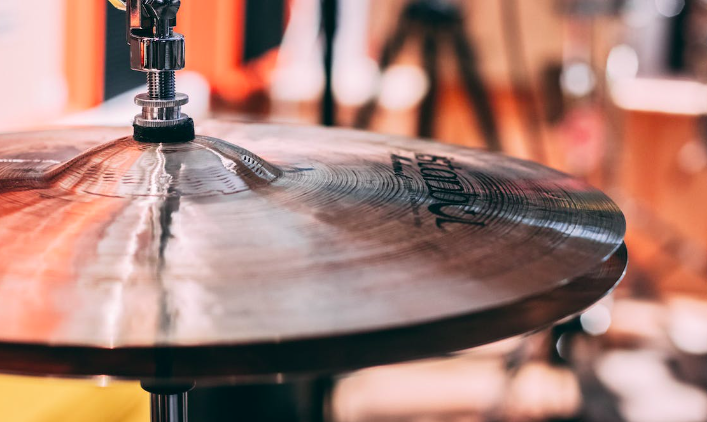
\includegraphics[width=2.77073in,height=2.73486in]{media/image1.png}

Há milhões de anos atrás, os humanos não existiam. Com o tempo, os
microrganismos que existiam no planeta terra deram origem a milhares de
espécies até chegarem em nós. Com o tempo, de seres individuais que
buscavam somente o próprio alimento, passamos a nos unir. Demos início à
nossa história, à história da humanidade. Formamos comunidades, que
viraram povos, que construíram cidades. Ocupamos o mundo e trabalhamos
muito tempo para chegar até aqui.

%Árvore de Araucária, que pode viver até 700 anos, e Formiga, que vive até 2 anos. 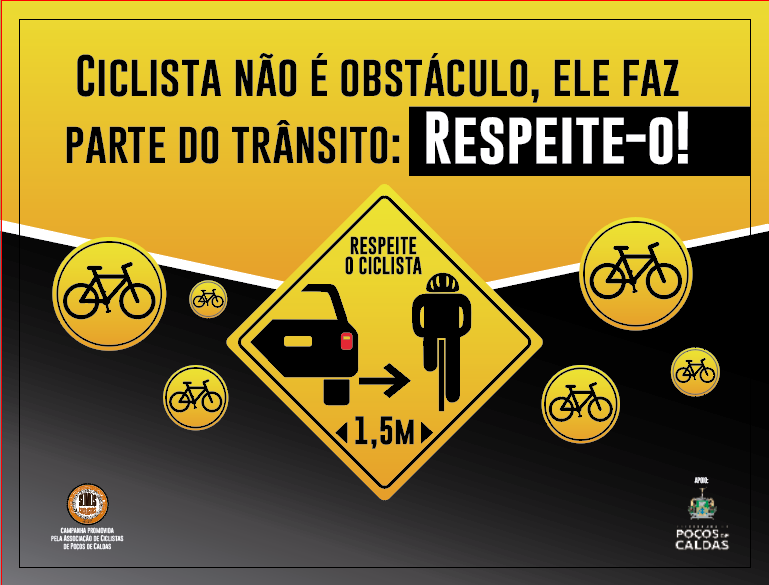
\includegraphics[width=3.27604in,height=2.18221in]{media/image2.png}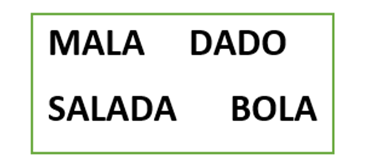
\includegraphics[width=2.90937in,height=2.17708in]{media/image3.png}

Para entender quem somos, como funciona nossa vida, e nossa sociedade,
precisamos lembrar que só somos quem somos e fazemos o que fazemos por
causa do tempo. Também, temos que saber que o tempo não é igual para
todos os seres. Para uma formiga que vive no máximo 2 anos, 1 ano é um
tempo muito grande, e representa metade da sua vida. Para uma árvore
Araucária, que pode viver até 700 anos, 1 ano é muito pouco. O tempo da
humanidade também é diferente do tempo do homem. A humanidade existe há
mais de 2 milhões de anos, enquanto o homem vive em média 70 anos.

São esses múltiplos tempos que vamos explorar neste módulo, e sua
relação com o espaço que habitamos.}

%Disponível em: {\emph{https://pixabay.com/pt/photos/formiga-inseto-animal-artr\%c3\%b3pode-1130497/}} Acesso em: 23 fev. 2023

%Disponível em: {\emph{https://pixabay.com/pt/photos/arauc\%c3\%a1ria-pinheiro-manh\%c3\%a3-sol-633196/}} Acesso em: 23 fev. 2023

\colorsec{Atividade 1}


\coment{Habilidade BNCC EF05HI0: Identificar os processos de formação das
culturas e dos povos, relacionando-os com o espaço geográfico ocupado.

Habilidades SAEB:

1A7: Reconhecer os aspectos históricos da ação do ser humano no tempo e
no espaço.

1B10: Relacionar a mudança de paisagens ou hábitos à passagem do tempo.}

Observe as imagens.

%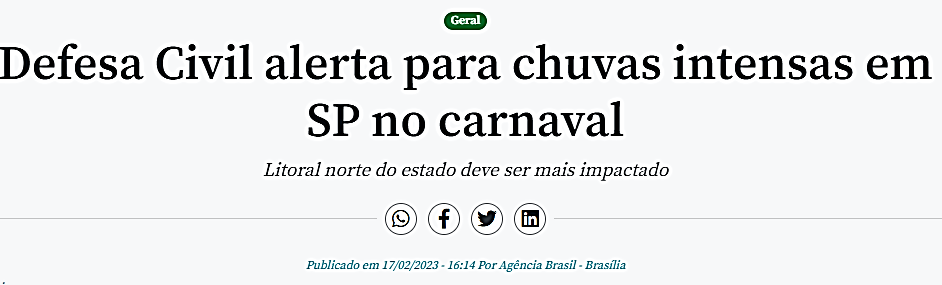
\includegraphics[width=6.26772in,height=3.86111in]{media/image4.png}

%Thierry Frères. Sequência do panorama da Baía do Rio de Janeiro, 1839, Biblioteca Nacional. Gravura litografia, 12,4 x 44,6cm em f. 52,6 x 34,6.

%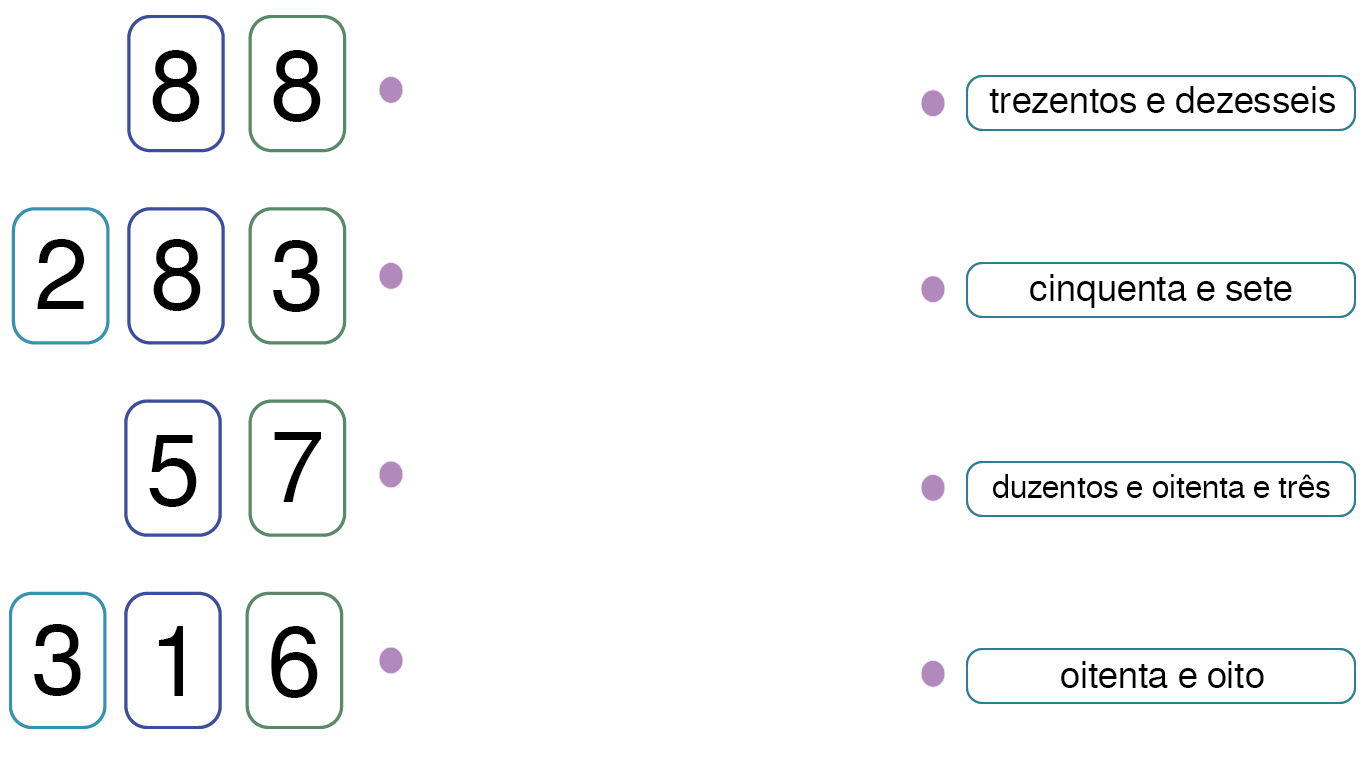
\includegraphics[width=6.26772in,height=3.16667in]{media/image5.png}

%Foto do Rio de Janeiro nos dias atuais.

As duas imagens representam o mesmo lugar, a Baía da cidade do Rio de
Janeiro, a primeira no ano de 1839, em uma gravura do artista Thierry
Frères, e a segunda em uma foto dos dias atuais.

\num{a} Quais mudanças você observa na imagem que ocorreram no espaço ao longo
do tempo? 

\linhas{3}
\coment{Espera-se que os alunos apontem as mudanças na paisagem natural, tomada
pelos edifícios.}

\num{b} Você sabe dizer o que aconteceu para que essas mudanças acontecessem?

\linhas{3}
\coment{Espera-se que o aluno fale sobre a ocupação do homem no espaço natural,
podendo tocar em questões como habitação, migração, urbanização,
crescimento econômico, etc.

Aqui, incentive os alunos a entenderem a ação humana enquanto
transformadora do espaço ao longo do tempo.}

\num{c} Você já se deparou com alguma mudança no bairro ou na cidade onde vive?
A construção de novas casas, escolas, comércios, etc? Descreva e discuta
com seus colegas.

\linhas{3}
\coment{Aqui os alunos devem trazer o debate para o seu cotidiano, falar sobre
as mudanças no espaço onde vive e perceber que ele está sempre em
construção e movimento ao longo do tempo.}

\colorsec{Atividade 2}

\coment{Habilidade BNCC EF05HI07: Identificar os processos de produção,
hierarquização e difusão dos marcos de memória e discutir a presença
e/ou a ausência de diferentes grupos que compõem a sociedade na nomeação
desses marcos de memória.

Habilidades SAEB:

1B3: Compreender o significado de objetos e documentos pessoais como
fontes de memórias e histórias.

1B6: Compreender o significado de marcos históricos na vida dos sujeitos
ou de grupos sociais.

1B20: Compreender o significado de objetos e documentos pessoais como
fontes de memórias e histórias nos âmbitos pessoal, familiar, escolar e
comunitário.

Recomenda-se que essa atividade seja feita em duplas ou grupos de 3 pessoas.}

Observe a imagem, leia a reportagem, e, depois, discuta com seus colegas.

%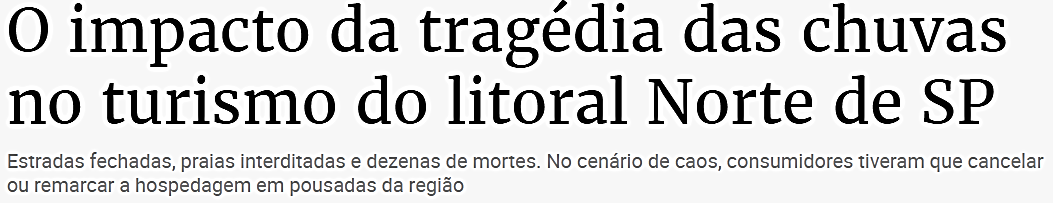
\includegraphics[width=4.75667in,height=2.67859in]{media/image6.png}

%{\emph{https://www.istockphoto.com/br/foto/antigo-cuneiforme-ass\%C3\%ADria-e-sum\%C3\%A9ria-da-mesopot\%C3\%A2mia-gm1128639883-297872773?phrase=escrita\%20cuneiforme}}

\begin{quote}
\textbf{O que diz o primeiro documento escrito da história}

Na Antiguidade, acreditava-se que a escrita vinha dos deuses. Os gregos
pensavam tê-la recebido de Prometeus. Os egípcios, de Tot, o deus do
conhecimento. Para os sumérios, a deusa Inanna a havia roubado de Enki,
o deus da sabedoria. Mas à medida que essa visão perdia crédito,
passou-se a investigar o que levou civilizações antigas a criar a
escrita.

As tábuas de argila adornadas com a primeira escrita abstrata do mundo
não haviam sido usadas para escrever poesia ou enviar mensagens a
lugares remotos. Foram empregadas para fazer contas - e também para
elaborar os primeiros contratos. Isso graças a uma combinação das peças
e da escrita cuneiforme que permitiu criar uma ferramenta brilhante: uma
bola oca de argila.

\fonte{Disponível em:
\emph{https://www.terra.com.br/byte/ciencia/o-que-diz-o-primeiro-documento-escrito-da-historia,91ff629390de632fb072b741c464fc55stmy8y08.html}
Acesso em: 22 fev. 2023.}
\end{quote}

\num{a} O que vocês entendem como um documento histórico?

\linhas{3}
\coment{Espera-se que o aluno tenha a compreensão do documento histórico como
uma fonte onde estão registrados acontecimentos, costumes, pensamentos
dos seres humanos, entre outros.}

\num{b} Porque vocês acham que documentos como o reproduzido na imagem acima são
importantes para nós hoje em dia?

\linhas{3}
\coment{Aqui, os alunos devem ter o entendimento de que a partir de documentos
como esse podemos conhecer aspectos do passado da humanidade e entender
sua formação, seu desenvolvimento e crescimento até chegarmos aqui.}

\num{c} Vocês acham que a descoberta escrita foi importante para os homens?
Porque? O que ela nos permite fazer em nosso dia a dia?

\linhas{4}
\coment{Essa questão requer que o aluno entenda a revolução do registro escrito
para o registro da memória humana. Podem aparecer respostas quanto ao
registro de contratos, como no texto, assim como questões mais amplas
como: expressão individual, registro de leis, de mercadorias,
comunicação, mandar recados, fazer provas, etc.}

\num{d} Marque com um X o que vocês acham que pode ser usado como um documento
histórico, depois, discutam com a sua professora e seus colegas o porquê
das suas escolhas.

\begin{boxlist}
\item
  Um livro de leis antigas
\item
  Uma obra de arte em um museu
\item
  Uma foto de família
\item
  Um texto nas redes sociais
\item
  Uma carta de amor
\item
  Uma letra de música
\item
  Um diário
\end{boxlist}

\coment{O ideal é que o aluno marque todas as alternativas. A ideia é que seja
discutido como qualquer registro da vida humana pode ser utilizado como
documento para entender a história dos homens. Assim, deve ser discutido
o poder da micro história, ou seja, o aluno deve entender que sua vida
pessoal, a de sua família, das pessoas de seu bairro, são reflexos de
aspectos históricos e também devem ser levadas em consideração.}

\colorsec{Atividade 3}

\coment{Habilidade BNCC: EF05HI08: Identificar formas de marcação da passagem do
tempo em distintas sociedades, incluindo os povos indígenas originários
e os povos africanos.

Habilidades SAEB:

1A4: Identificar formas de marcação da passagem do tempo em distintas
sociedades, incluindo os povos indígenas originários e os povos
africanos.

1B5: Utilizar diferentes marcadores do tempo, como relógio e calendário.}

%Disponível em: {\emph{https://pixabay.com/pt/photos/calend\%c3\%a1rio-asteca-asteca-escultura-642655/}} Acesso em: 23 fev. 2022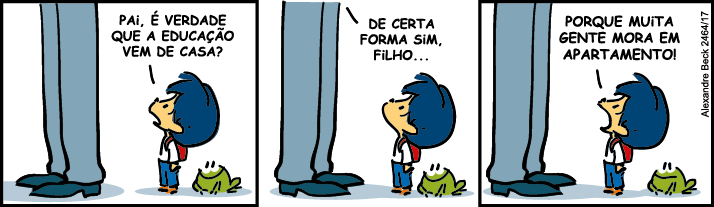
\includegraphics[width=3.56599in,height=2.36609in]{media/image7.png}

Você sabia que cada sociedade construiu seu próprio calendário? A imagem
ao lado representa o calendário da sociedade Asteca, que viveu no
território de onde hoje é o México entre os anos de 1300 e 1500 d.C. Ele
é dividido em duas partes: uma baseada no ciclo do sol, que era
utilizada para guiar os ciclos da agricultura, composta por 365 dias, e
a outra, de 260 dias, que guiava os rituais sagrados. O calendário que
utilizamos hoje em dia na sociedade ocidental vem da sociedade romana, e
foi criado em meados de 700 d.C. O calendário mais antigo do mundo é o
chinês, baseado nos ciclos da lua e do sol, e um ciclo completo tem a
duração de 12 anos. O ano novo chinês, por exemplo, não é comemorado no
dia 1 de janeiro, como estamos acostumados, mas sim entre os meses de
janeiro e fevereiro, cada ano em um dia diferente. Texto original

Existem também calendários dos povos indígenas brasileiros. Vamos ver
como um deles funciona:

O calendário anual indígena enfatiza certos fenômenos e ciclos
biológicos particulares como referência. Nomeadamente, o ciclo
hidrológico (precipitações e, sobretudo, as flutuações no nível dos
rios); o ciclo de vida dos peixes, especialmente de algumas espécies de
aracus (gênero Leporinus) e o calendário agrícola. O ano para os povos
indígenas do rio Tiquié, no Noroeste Amazônico, divide-se em várias
estações, identificadas a partir da passagem de constelações
astronômicas associadas a diversos processos ecossistêmicos e
climáticos. O ano começa com a Enchente de Jararaca, no começo de
novembro. Essa região é caracterizada por muita chuva distribuída por
todo o ano, com alguns curtos períodos de estiagem.

%Disponível em: {\emph{https://infoamazonia.org/project/calendario-indigena-dos-ciclos-do-rio-tiquie/}} Acesso em: 24 fev. 2023

\num{a} O que é um calendário? Qual a sua função em cada sociedade?

\linhas{3}
\coment{Aqui, o aluno deve falar sobre o calendário e sua relação com a marcação
do tempo e com a organização da sociedade.}

\num{b}Qual é a principal importância do calendário para o povo indígena
brasileiro descrito no texto?

\linhas{3}
\coment{Aqui, espera-se que o aluno fale sobre a relação dos povos indígenas
brasileiros com o clima e com as estações do ano.}

\num{c} Aponte duas características de cada calendário mencionado nos textos:

Calendário Asteca:

\begin{enumerate}
\item \coment{agricultura baseada no ciclo do sol}

\item \coment{função religiosa e sagrada}
\end{enumerate}

Calendário Romano:

\begin{enumerate}
\item 

\item 
\end{enumerate}

\coment{Aqui o aluno pode colocar qualquer característica do calendário
ocidental atual: 12 meses, 4 estações, 365 dias, etc. As informações não
estão no texto, então a professora deve lembrar que este é o calendário
que eles utilizam no dia a dia.}

Calendário Chinês:

\begin{enumerate}
\item \coment{Baseados no ciclo da lua e do sol}

\item \coment{Duração de 12 anos}
\end{enumerate}

Calendário indígena brasileiro:

\begin{enumerate}
\item \coment{Dividido por estações}

\item \coment{baseado em aspectos da natureza (peixes, chuvas, etc)}
\end{enumerate}

\colorsec{Treino}

\num{1} A micro-história caracteriza-se pela ``microanálise'', isto é, a
análise de elementos do passado histórico em nível de escala muito
reduzido, tendo como alvo aspectos culturais, econômicos e sociais. Um
exemplo é a análise da vida de pessoas comuns, que, em vida, nunca
tiveram nenhuma notoriedade, como camponeses pobres da Idade Média ou do
início da Idade Moderna.

Um objeto da micro-história, além dos camponeses da Idade Média como
aponta o texto, pode ser:

\begin{escolha}
\item as decisões de presidentes importantes.

\item as guerras entre grandes sociedades.

\item o cotidiano de empregadas domésticas.

\item a ocupação de continentes desconhecidos.
\end{escolha}

\fonte{Disponível em:
\emph{https://brasilescola.uol.com.br/historia/importancia-micro-historia-italiana.htm}
Acesso em: 23 fev. 2023.}

\coment{Habilidade BNCC EF05HI07: Identificar os processos de produção,
hierarquização e difusão dos marcos de memória e discutir a presença
e/ou a ausência de diferentes grupos que compõem a sociedade na nomeação
desses marcos de memória.

SAEB: 1B6: Compreender o significado de marcos históricos na vida dos
sujeitos ou de grupos sociais.

a) Incorreta. Os presidentes de países importantes tem impacto em
questões de grande escala mundial, e suas decisões situam-se no nível
Macro;
b) Incorreta. Guerras entre grandes sociedades afetam também as
populações ao redor em grande escala, compondo o nível macro;
c) Correta. A micro-história é a história do cotidiano e de personagens
que, originalmente, não estão nos livros de história, como as empregadas
domésticas;
d) Incorreta. A ocupação de continentes, como a da América pelos
Europeus, faz parte da macro-história}

\num{2}

\begin{quote}
\textbf{Dicionário histórico dos nomes das ruas de Guarulhos - São Paulo}

Tipo: Rua\\
Denominação atual: Rua Inhuma\\
Denominação antiga: Rua Cinco\\
Bairro: Vila Dinamarca, Água Chata\\
Ato legal: Decreto nº 5.168, de 31 de dezembro de 1975\\
Verbete: Sua denominação pode ser entendida a partir de duas
referências. A primeira faz alusão à cidade de Inhuma, no estado do
Piauí, e a segunda à ave anhuma, também conhecida como inhuma, presente
na bandeira de Guarulhos. Inhuma é um termo de origem tupi e significa
ave ou pássaro preto. O município piauiense localiza-se a
aproximadamente 259 km da capital, Teresina. A possibilidade de a rua
ter recebido esse nome em homenagem ao município piauiense é grande,
Guarulhos e outras regiões a leste da cidade de São Paulo receberam
grande migração nordestina. Quanto à ave, é símbolo do estado de Goiás.
É nativa da América do Sul, vivendo em áreas à beira de rios, lagos e
mangues.

\fonte{Disponível em:
\emph{https://dicionarioruasguarulhos.wordpress.com/rua-inhuma/}
Acesso em: 23 fev. 2023.}
\end{quote}

Como aponta o texto, o nome da Rua Inhuma na cidade de Guarulhos pode
ter sido dado por dois motivos:

\begin{escolha}
\item hábitos alimentares e as vestimentas tradicionais.

\item importância do comércio e cultura popular.

\item origem dos moradores e o símbolo da cidade.

\item localização na cidade e formato das casas.
\end{escolha}

\coment{BNCC EF05HI0: Identificar os processos de formação das culturas e dos
povos, relacionando-os com o espaço geográfico ocupado.

SAEB: 1C2. Discutir os critérios que explicam a escolha do nome de ruas,
monumentos e edifícios.

a) Incorreta. Não há indícios sobre a nomeação baseada na alimentação ou
vestimenta dos moradores;
b) Incorreta. Não é dada importância à economia na rua, nem à cultura
popular de forma geral;
c) Correta. De fato, a origem nordestina dos moradores e Inhuma como
símbolo da cidade de Guarulhos são os fatores responsáveis pela
nomeação;
d) Incorreta. Não há menção à localização como fator, nem à arquitetura
das moradias.}

\num{3}

\begin{quote}
Chove muito, o verão não acontece. A roça também não queima, porque a
chuva é muita. Nossos avôs já diziam isso. Parece que a nossa época não
é boa, por isso a chuva não para de cair.

Antes não era assim. Antigamente, quando meu pai ainda era vivo, não era
como agora. Só agora é desse jeito... Por que o tempo de hoje se
transformou?

Talvez nosso dono altere o tempo de hoje, o tempo vai mudar, por isso
chove muito. Nosso dono vai trocar a terra. A terra será renovada, disse
o nosso dono, por isso a terra queimará. A terra queimará...

\fonte{Disponível em:
\emph{https://pib.socioambiental.org/pt/\%22O\_tempo\_vai\_mudar,\_por\_isso\_chove\_muito.\_Nosso\_dono\_vai\_trocar\_a\_terra\%22}
Acesso em: 23 fev. 2023}
\end{quote}

A declaração do indígena Seremete Wajãpi mostra que, para sua comunidade, o tempo está diretamente ligado a

\begin{escolha}
\item acontecimentos da natureza.

\item guerras entre povos.

\item rituais de cura.

\item relações das famílias.
\end{escolha}

\coment{Habilidade BNCC: EF05HI08: Identificar formas de marcação da passagem do
tempo em distintas sociedades, incluindo os povos indígenas originários
e os povos africanos.

Habilidades SAEB:

1A4: Identificar formas de marcação da passagem do tempo em distintas
sociedades, incluindo os povos indígenas originários e os povos
africanos.

1B5: Utilizar diferentes marcadores do tempo, como relógio e calendário.

a) Correta. De fato, o autor faz referência a mudança do tempo enquanto
ligada aos acontecimentos naturais como a chuva e a queima da terra;
b) Incorreta. Não é mencionada a guerra e nem conflitos com outros
povos;
c) Incorreta. Não é falado sobre doenças ou a cura destas;
d) Incorreta. Apesar de mencionar os avós e os pais, o indígena não os
relaciona com a mudança do tempo, somente os situa dentro dele.}

\chapter{2. Natureza e questões socioambientais}

\coment{Habilidades da BNCC envolvidas: EF05GE03 EF05GE10 EF05GE11 EF05GE12}

\conteudo{O homem está separado da natureza? O lugar em que vivemos faz parte das
florestas, campos, rios e mares onde vivem os animais? Mesmo que não
vivamos em nosso dia a dia em contato direto com a natureza, nossas
ações impactam na preservação ou na destruição dela ao nosso redor. Tudo
que usamos em nosso dia a dia vem da natureza. Esta folha de papel, por
exemplo, em que você está lendo este texto, veio de uma árvore, assim
como o lápis que está no seu estojo. Isso quer dizer que estamos
destruindo a natureza escrevendo em nossos cadernos? Não, mas quer dizer
que precisamos trabalhar pelo equilíbrio do uso de nossos recursos
naturais. Devemos sempre pensar em como podemos passar por esse processo
de maneira \textbf{sustentável}.

Mas como ser sustentável? O que isso significa?

%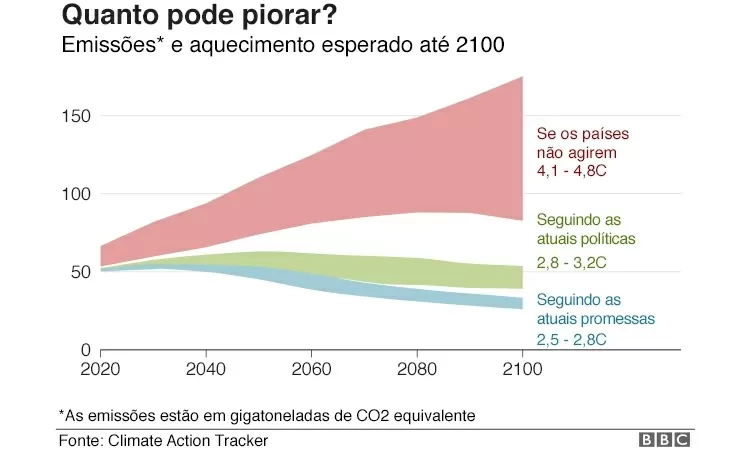
\includegraphics[width=6.36147in,height=4.21344in]{media/image8.png}
%\emph{https://br.freepik.com/fotos-gratis/menina-asiatica-segurando-planta-e-solo\_5598508.htm\#query=preserva\%C3\%A7\%C3\%A3o\&position=9\&from\_view=search\&track=sph}

Para ser sustentável precisamos garantir que, mesmo utilizando os
recursos naturais para nossa vida no presente, eles não acabem. Isso
porque as pessoas vão precisar deles no futuro! Imagine se há 50 anos
atrás nossos avós tivessem acabado com todas as árvores do planeta! E
tivessem usado toda água potável do mundo? Como viveríamos hoje?

Neste módulo vamos trabalhar com atividades que relacionam a vida humana
com a natureza. Afinal, somos todos parte do mesmo planeta, e precisamos
um do outro para sobreviver.}

\colorsec{Atividade 1}

\coment{Habilidade BNCC EF05GE03}

Vamos ler essa reportagem de 2020.

\begin{quote}
\textbf{Expansão urbana provoca encontros incomuns com onças-pardas}

Imagine a emoção de ficar frente a frente com uma onça. Com certeza a
adrenalina predomina no instante do encontro. No entanto, quando o
flagrante é feito em áreas urbanas, um sinal vermelho se acende, afinal,
esse não é o habitat ideal para um felino selvagem. Infelizmente estes
casos são cada vez mais frequentes devido à expansão urbana desenfreada,
construções de rodovias que dividem áreas verdes e desmatamento
constante.

``É importante que ele seja reintroduzido logo, para buscar o habitat
natural. Devemos trabalhar essa consciência ambiental e atuar de forma
correta para que a gente não prejudique nem a natureza e nem o animal,
que não tem culpa de nada do que está acontecendo''.

\fonte{\emph{https://g1.globo.com/sp/campinas-regiao/terra-da-gente/noticia/2020/01/29/expansao-urbana-provoca-encontros-incomuns-com-oncas-pardas.ghtml}}
\end{quote}

Agora, vamos investigar melhor esse fenômeno

\num{a} Qual você acha que foi a principal ação humana responsável por esse
acontecimento?

\linhas{3}
\coment{Espera-se que o aluno fale sobre a expansão urbana na natureza, sobre o
crescimento das cidades e a ocupação de territórios em que,
originalmente, habitavam animais selvagens.}

\num{b} Como você acha que o crescimento de áreas urbanas afeta a natureza e os
animais que vivem ao redor?

\linhas{3}
\coment{Aqui, proponha uma reflexão tanto sobre a fauna quanto a flora. Faça os
alunos refletirem sobre questões mais amplas como desmatamento,
poluição, invasão territorial, etc.}

\num{c} Você acha que a expansão urbana pode trazer perigo aos próprios seres
humanos? Se sim, porquê?

\linhas{3}
\coment{Aqui, volte ao conteúdo da reportagem do caso da onça parda. Fale sobre
os perigos do contato entre homens e animais selvagens. Objetiva-se que
o aluno entenda que as ameaças da expansão urbana desenfreada não estão
restritas aos animais.}

\colorsec{Atividade 2}

\coment{Habilidade BNCC EF05GE11 / Habilidade SAEB 2 B8}

Agora, observe a imagem, e, seguida, leia a reportagem de 2022.

%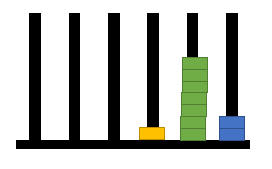
\includegraphics[width=6.26772in,height=3.68123in]{media/image9.png}
%\fonte{\emph{https://br.freepik.com/vetores-gratis/cartaz-de-aquecimento-global-com-crianca-e-fabrica\_5837841.htm\#query=polui\%C3\%A7\%C3\%A3o\%20escola\&position=8\&from\_view=search\&track=ais}}

\begin{quote}
Poluição em escolas em Diadema, na Grande SP, é quase três vezes maior
do que o recomendado, aponta pesquisa.

Um estudo realizado em cinco escolas públicas de Diadema, na Grande São
Paulo, mostra que os níveis de poluentes no ar da cidade estão muito
acima do normal. O nível de poluição está em 40 microgramas diários de
poluentes e, segundo a Organização Mundial da Saúde (OMS), o
recomendável seria ter até 15 microgramas. Para medir o nível de
poluição, as escolas receberam um equipamento para monitorar os
poluentes.

"Foi uma surpresa porque a nossa escola é bastante arborizada e, quando
vimos os resultados, foi surpreendente. Imaginávamos que fosse melhor.",
afirma Carolina de Paula Lusa, diretora da escola municipal de educação
básica Carolina Maria de Jesus.

\fonte{Disponível em: \emph{https://g1.globo.com/sp/sao-paulo/noticia/2022/07/06/poluicao-em-escolas-em-diadema-na-grande-sp-e-quase-tres-vezes-maior-do-que-o-recomendado-aponta-pesquisa.ghtml}
Acesso em: 23 fev. 2023}
\end{quote}

\num{a} Descreva o que você observa na imagem.

\linhas{3}
\coment{Espera-se que o aluno descreva o ambiente urbano e seus componentes, os
carros e as indústrias, além das personagens humanas e suas expressões.}

\num{b} Na sua opinião, como podemos relacionar os elementos da imagem ao
acontecimento relatado na reportagem?

\linhas{3}
\coment{Aqui, o aluno deve relacionar a poluição observada na imagem em
decorrência dos automóveis e indústrias com a qualidade do ar observada
na escola.}

\num{c} Como podemos explicar, no caso de Diadema, que mesmo a escola tendo
bastante árvores, os níveis de poluentes estão acima do normal?

\linhas{3}
\coment{Espera-se que o aluno situe a escola dentro do ambiente da cidade, ou
seja, que ele entenda que as interferências humanas no ambiente externo
à escola afetam o perímetro escolar. Mesmo a escola sendo urbanizada,
podem haver indústrias, automóveis, e outros fatores ao redor da escola
que comprometam a salubridade naquele local.}

\num{d} Qual o perigo que a poluição do ar traz para as crianças nas escolas?

\linhas{2}
\coment{Como na imagem acima, as crianças podem ficar doentes e ter a qualidade
da respiração afetada pelo ar poluído, tornando o ambiente escolar
frequentado todos os dias por elas insalubre.}

\num{e} Marque com um X as medidas do governo e da população que podem ajudar na
diminuição da poluição do ar nas cidades:

\begin{boxlist}
\item
  Incentivar o uso de transportes coletivos. \coment{X}
\item
  Diminuir as queimadas em plantações. \coment{X}
\item
  Asfaltar as ruas da cidade.
\item
  Plantar árvores em áreas desmatadas. \coment{X}
\item
  Melhorar o sistema de esgoto.
\end{boxlist}

\coment{Nesta etapa da atividade, é interessante que sejam debatidos com os
alunos cada ponto colocado, entendendo no que exatamente eles auxiliam a
sociedade. Os transportes, pela diminuição de emissão de poluentes em
carros privados, as queimadas, pela diminuição da emissão de gases
tóxicos que resultam da ação, e as árvores, pois elas melhoram a
qualidade do ar a partir do processo de fotossíntese.}

\colorsec{Atividade 3}

\coment{Habilidade BNCC EF05GE10: Reconhecer e comparar atributos da qualidade
ambiental e algumas formas de poluição dos cursos de água e dos oceanos
(esgotos, efluentes industriais, marés negras etc.).

Recomenda-se que essa atividade seja feita em grupos. Isso para que os
alunos compartilhem suas experiências e, juntos, busquem por soluções.}

Observe as imagens e responda às questões com seus colegas.

%Imagem 1 Imagem 2 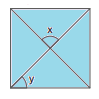
\includegraphics[width=3.65127in,height=2.42708in]{media/image10.png}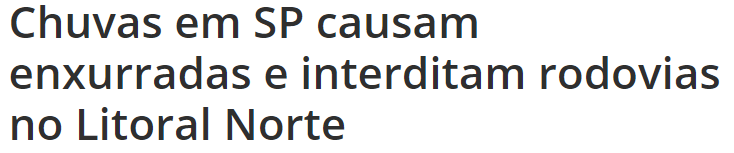
\includegraphics[width=2.78646in,height=2.42246in]{media/image11.png}

%\emph{https://br.freepik.com/fotos-gratis/lixo-na-areia-da-praia-mostrando-o-problema-de-poluicao-ambiental\_3805894.htm\#query=praia\%20polu\%C3\%ADda\&position=3\&from\_view=search\&track=ais}

%\emph{https://br.freepik.com/vetores-gratis/poluicao-da-agua-com-sacos-de-plastico-no-oceano\_7026496.htm\#query=mar\%20polu\%C3\%ADdo\&position=7\&from\_view=search\&track=ais}

\num{a} Você já foi ou conhece alguém que foi à praia? Se sim, como você ou essa
pessoa descreveriam essa experiência e a paisagem? Se não, como você
imagina que seria?

\linhas{4}
\coment{Essa questão pretende iniciar o debate entre os alunos. Lembrando de
suas experiências, eles poderão se relacionar de maneira pessoal com as
questões em seguida.}

\num{b} Agora, descrevam o que vocês vêem nas imagens acima.

\linhas{3}
\coment{Espera-se que os alunos apontem a grande quantidade de resíduos
descartados nas paisagens.}

\num{c} Como vocês acham que a imagem 1 se relaciona com a imagem 2?

\linhas{3}
\coment{Aqui, espera-se que o aluno relacione a causa à consequência: ao jogar
lixo na praia, estão colaborando para o acúmulo de lixo no fundo do mar.}

\num{d} Quais os impactos que a ação de jogar lixo na praia tem sobre a natureza
e os animais que vivem nela? Cite três.

\begin{enumerate}
\item \linhas{2}

\item \linhas{2}

\item \linhas{2}
\end{enumerate}

\coment{Estimule os alunos a pensar nas consequências dessa ação tanto para o
homem quanto para os animais e a vegetação local. Podem ser citados:
turismo, morte de animais e risco de extinção de espécies, poluição da
água do mar e dos peixes a serem consumidos pelos humanos, etc.}

\num{e} Converse com os colegas e aponte duas ações que podem ser feitas para
diminuir o lixo nas praias e mares.

\linhas{3}
\coment{Aqui podem entrar tanto ações individuais, como descartar o lixo em
local adequado quando visitar a praia, quanto governamentais, como
promover ações de retirada do lixo das praias, estimular a reciclagem,
etc.}

\colorsec{Treino}

\num{1}

\begin{quote}
\textbf{Ubatuba começa a cobrar taxa ambiental de R\$ 13 por veículo
nesta quarta-feira}

A cobrança da taxa será feita por um sistema semelhante ao da cobrança
eletrônica (Sem Parar) dos pedágios de rodovias, instalados nos
principais acessos da cidade.

A partir da zero hora desta quarta-feira, 8, turistas e visitantes terão
de pagar taxa para permanecer por mais de 4 horas em Ubatuba, no litoral
norte de São Paulo. A cidade, um dos principais destinos do verão
paulista, tem 102 praias catalogadas. A prefeitura criou uma taxa de
preservação ambiental para compensar os impactos gerados pelo alto fluxo
de turistas, sobretudo na alta temporada, como agora. A tarifa básica
para carros é de R\$ 13 por período (entrada e saída).

\fonte{Disponível em: \emph{https://exame.com/}
Acesso em: 6 fev. 2023}
\end{quote}

Segundo o texto, a cobrança da taxa ambiental pela prefeitura tem como
objetivo

\begin{escolha}
\item aumentar o número de turistas na região.

\item controlar a criminalidade na cidade.

\item diminuir o consumo de peixes e frutos do mar.

\item garantir a preservação das praias locais.
\end{escolha}

\coment{Habilidades BNCC:

EF05GE10: Reconhecer e comparar atributos da qualidade ambiental e
algumas formas de poluição dos cursos de água e dos oceanos (esgotos,
efluentes industriais, marés negras etc.).

EF05GE12: Identificar órgãos do poder público e canais de participação
social responsáveis por buscar soluções para a melhoria da qualidade de
vida (em áreas como meio ambiente, mobilidade, moradia e direito à
cidade) e discutir as propostas implementadas por esses órgãos que
afetam a comunidade em que vive.

Habilidade SAEB 2C1: Julgar as vantagens ou os riscos da intervenção
humana na natureza.

a) Incorreta. A prefeitura não visa aumentar o número de turistas, mas
controlar o impacto da vinda de turistas sobre a natureza;
b) Incorreta. Não existe relação entre a taxa ambiental e a
criminalidade na cidade;
c) Incorreta. Não existem evidências no texto sobre o consumo de
alimentos;
d) Correta. De fato, a taxa visa compensar os impactos dos turistas
sobre as praias locais.}

\num{2} Observe a imagem.

%
\includegraphics[width=6.21354in,height=3.29722in]{media/image12.jpg}

%\emph{https://br.freepik.com/vetores-gratis/conjunto-de-triagem-de-lixo\_13146308.htm\#query=reciclagem\&position=4\&from\_view=search\&track=sph}

A imagem acima ilustra um elemento que impacta o seguinte processo:

\begin{escolha}
\item saneamento básico.

\item industrialização.

\item reciclagem.

\item urbanização.
\end{escolha}

\coment{Habilidade BNCC:

EF05GE11: Identificar e descrever problemas ambientais que ocorrem no
entorno da escola e da residência (lixões, indústrias poluentes,
destruição do patrimônio histórico etc.), propondo soluções (inclusive
tecnológicas) para esses problemas.

EF05GE12: Identificar órgãos do poder público e canais de participação
social responsáveis por buscar soluções para a melhoria da qualidade de
vida (em áreas como meio ambiente, mobilidade, moradia e direito à
cidade) e discutir as propostas implementadas por esses órgãos que
afetam a comunidade em que vive.

Habilidade SAEB: 2C4: Propor soluções adequadas ao descarte de lixo nas
cidades.

a) incorreta. A imagem não se relaciona ao saneamento, mas sim à
reciclagem;
b) incorreta. A imagem não influi no sistema industrial, mas no descarte
do lixo;
c) correta. A imagem mostra o processo de separação do lixo, parte da
reciclagem;
d) incorreta. A imagem não dá sinais de impactar a ambientação urbana.}

\num{3}

\begin{quote}
\textbf{Estatuto da Cidade, Lei No 10.257, de 10 de julho de 2001}

Art. 2º A política urbana tem por objetivo
ordenar o pleno desenvolvimento das funções sociais da cidade e da
propriedade urbana, mediante as seguintes diretrizes gerais:

XVII - estímulo à utilização, nos parcelamentos do solo e nas
edificações urbanas, de sistemas operacionais, padrões construtivos e
aportes tecnológicos que objetivem a redução de impactos ambientais e a
economia de recursos naturais.
\end{quote}

O trecho do Estatuto da Cidade reproduzido acima tem como objetivo
equilibrar o desenvolvimento urbano com o (a)

\begin{escolha}
\item ampliação das escolas.

\item crescimento da população.

\item preservação da natureza.

\item produção de alimentos.
\end{escolha}

\coment{Habilidade BNCC EF05GE03: Identificar as formas e funções das cidades e
analisar as mudanças sociais, econômicas e ambientais provocadas pelo
seu crescimento.

Habilidade SAEB: 2A2 e 2B8

a) Incorreta. Esse trecho da lei não menciona as escolas quando aborda o
contexto urbano;
b) Incorreta. O trecho não fala sobre crescimento populacional;
c) Correta. De fato, o trecho busca incentivar sistemas e tecnologias
construtivas no ambiente urbano que diminuam os impactos à natureza;
d) Incorreta. O trecho não menciona políticas de produção alimentícia.}

\chapter{3. Culturas, identidades e diversidades}

\coment{Habilidades da BNCC envolvidas:

EF05GE02: Identificar diferenças étnico-raciais e étnico-culturais e
desigualdades sociais entre grupos em diferentes territórios.

EF05HI03: Analisar o papel das culturas e das religiões na composição
identitária dos povos antigos.

EF05HI10: Inventariar os patrimônios materiais e imateriais da
humanidade e analisar mudanças e permanências desses patrimônios ao
longo do tempo.}

%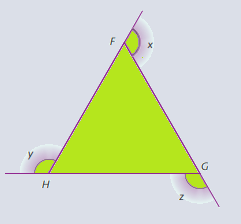
\includegraphics[width=6.26772in,height=4.18056in]{media/image13.png}
%\emph{https://br.freepik.com/vetores-gratis/fundo-plano-de-dia-de-paz-com-as-criancas\_5189550.htm\#query=crian\%C3\%A7a\%20cultura\&position=4\&from\_view=search\&track=ais}

\conteudo{Todas as pessoas do planeta vivem de maneira igual? Você acorda, vive o
dia, se alimenta, e dorme todos os dias. Isso parece ser igual para
você, para mim, e para uma pessoa do outro lado do planeta. Isso quer
dizer que somos iguais? Apesar de sermos todos seres humanos, o modo
como levamos nossas vidas depende de vários fatores. Por exemplo: uma
criança que nasce em uma comunidade na beira do rio, está muito mais
acostumada a comer peixe no seu dia a dia do que uma criança nascida em
uma fazenda no interior, que come ovos de galinha e carne de boi. Uma
criança que vive em uma cidade muito fria, se veste com roupas muito
mais pesadas do que uma criança que vive em uma cidade muito quente. O
que comemos, o modo como nos vestimos, como aproveitamos a vida, depende
do lugar onde crescemos.

Neste módulo vamos trabalhar para entender nossas diferenças e
semelhanças, de onde vem nossa cultura e como podemos viver em
comunidade e respeitar o próximo.}

\colorsec{Atividade 1}

\coment{EF05HI10: Inventariar os patrimônios materiais e imateriais da
humanidade e analisar mudanças e permanências desses patrimônios ao
longo do tempo.

SAEB

3A6: Identificar diferentes tipos de apropriações e usos culturais dos
espaços públicos.

3B3:Compreender os processos de formação das culturas e dos povos e suas
relações com o espaço geográfico ocupado.

3C5: Explicar as origens de costumes ou tradições de populações de
diferentes regiões do Brasil.}

Observe as imagens, leia a reportagem sobre o Carnaval e, em seguida,
discuta com os colegas.

%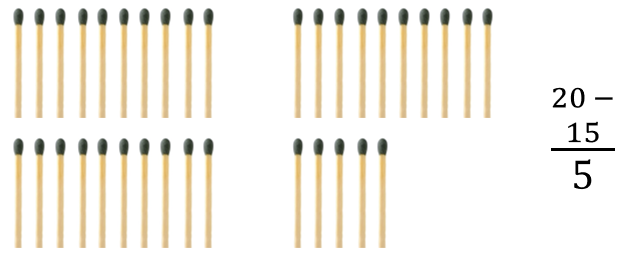
\includegraphics[width=4.23438in,height=2.82057in]{media/image14.png}
%\emph{https://pixabay.com/pt/photos/pessoas-multid\%c3\%a3o-celebra\%c3\%a7\%c3\%a3o-6622786/}

%\emph{https://www.pexels.com/pt-br/foto/homem-vestindo-camisa-polo-branca-e-chapeu-1974100/} 
\includegraphics[width=4.77604in,height=3.17345in]{media/image15.png}

\begin{quote}
Em 1846, já existia uma prática que foi absorvida ao Carnaval: o Zé
Pereira, que era uma pessoa que saía andando pelas ruas batendo bumbo e
tambores. Foi um dos pontos que acrescentou a música ao Entrudo. O ``Zé
Pereira'' era considerado um ``Carnaval do Pobre'', já que não era
preciso convite ou grandes organizações, bastava uma pessoa e um tambor
para a festa começar nas ruas.

No início do século 20, a festa de rua mudou nas capitais brasileiras.
Isso porque a própria rua mudou. No Rio de Janeiro, por exemplo, a
Avenida Central foi aberta entre 1903 e 1906. O espaço passou das ruas
estreitas para as largas avenidas. Apenas para abrir a Avenida Central,
foram demolidas entre 600 e 3 mil casas, desabrigando mais de 20 mil
pessoas mais pobres, levando-as para regiões mais afastadas.

Embora tenha sido idealizada para que os ricos desfrutassem da capital
do Brasil, a reurbanização trouxe também os mais pobres para aproveitar
as ruas e calçadas nos dias de folga. O Carnaval e o urbanismo se
encontraram. A Avenida Central, feita com calçadas largas, tinha os
pedestres e o comércio em foco. E, durante o Carnaval, tornou-se o eixo
dos blocos e cordões. Em Salvador, o mesmo aconteceu na Avenida Sete de
Setembro e em volta do Farol da Barra.

\fonte{Disponível em:
\emph{https://habitability.com.br/carnaval-e-urbanismo-uma-historia-que-se-mistura-no-brasil/}
Acesso em: 23 fev. 2023}
\end{quote}

\num{a} Você sabe o que é carnaval? Já participou de algum? Escreva e
compartilhe sua experiência com seus colegas.

\linhas{3}
\coment{Espera-se que os alunos tragam experiências pessoais, falem do que
entendem por carnaval. Cabe ao docente guiar a discussão.}

\num{b} O que a figura de "Zé Pereira" simboliza dentro das comemorações de
carnaval?

\linhas{3}
\coment{Aqui, a professora deve guiar a reflexão dos alunos, pois se trata de
uma associação um pouco mais complexa. Deve-se falar sobre a relevância
e importância do povo para esta comemoração. Zé pereira simboliza o
cidadão comum, que manifesta a cultura do carnaval de rua. A professora
pode falar também sobre a importância da ocupação do espaço da rua por
este personagem.}

\num{c} Qual é a ação do governo descrita pelo texto na cidade que muda o
funcionamento do carnaval no Rio de Janeiro ao longo do tempo?

\linhas{2}
\coment{Aqui o aluno deve falar sobre a abertura das ruas e a criação de largas
avenidas.}

\num{d} Cite uma consequência negativa e uma positiva dessa mudança.

\linhas{3}

\coment{Negativa: Desabrigou pessoas.

Positiva: Maior espaço de reunião da população nas festividades.
Ocupação em massa do espaço público.}

\num{e} Você já viu outros tipos de eventos em seu bairro ou em sua cidade que
ocuparam e fecharam as ruas? Cite e discuta com os colegas.

\linhas{2}
\coment{Aqui espera-se que os alunos busquem na memória situações em que viram
as ruas ocupadas pela população, como feiras de rua, festas de São João,
festas de ano novo, manifestações populares, eventos esportivos, etc.}

\colorsec{Atividade 2}

\coment{Habilidade BNCC EF05GE02: Identificar diferenças étnico-raciais e
étnico-culturais e desigualdades sociais entre grupos em diferentes
territórios.

Habilidade SAEB: 3A7: Identificar diferenças étnico-raciais e culturais
entre grupos em situações de desigualdade socioespacial.}

Leia os textos a seguir sobre o Projeto Integrado Entrada da Cidade
(Piec), projeto da prefeitura da cidade de Porto Alegre, no Rio Grande
do Sul.

\begin{quote}
\textbf{Texto 1}\\
\textbf{Entrada da Cidade, cara nova na chegada à Capital}

O Projeto Integrado Entrada da Cidade (Piec) visa ao desenvolvimento
urbano, socioeconômico e ambiental da Região Humaitá-Navegantes, com um
investimento de R\$ 140 milhões. As ações voltadas à habitação atendem
3.775 famílias com um investimento de R\$ 71,4 milhões; 3.061 são novas
casas e 714 lotes urbanizados.

\fonte{Disponível em:
\emph{http://www2.portoalegre.rs.gov.br/demhab/default.php?p\_secao=101}
Acesso em: 23 fev. 2023.}
\end{quote}

\begin{quote}
\textbf{Texto 2}\\
A referência ao ``morro'' e ao ``asfalto'' é talvez uma das imagens mais
utilizadas para indicar a divisão entre pobres e ricos nas cidades
brasileiras. Se estas imagens funcionam como representações das
delimitações espaciais entre pobres e ricos, elas também generalizam o
que há no asfalto e no morro. A implementação do PIEC junto aos
moradores e especificamente com relação à questão das moradias consistiu
na mudança das famílias que viviam em áreas consideradas ``de risco''
para os novos condomínios residenciais. Ao andar pelas ruas da Entrada
da Cidade (EC) atentando ao pertencimento racial das famílias que moram
ali é possível identificar uma certa geografia racial vivida no
cotidiano, ou se preferirmos, é possível identificar o papel da
identidade racial na configuração da geografia daquele espaço. A
espacialização que divide algumas famílias na EC configura uma
``espacialização racializada'', já que situou famílias negras nos fundos
e famílias não negras na parte da frente dos terrenos. Se, por um lado,
viver nos novos condomínios implica em sair da situação de viver em
banhados e nos fundos da casa de alguém, por outro, não há, até o
presente momento indicações de que houvesse diminuído as tensões e as
desvantagens existentes entre as famílias negras e a vizinhança
não-negra daquela área.

\fonte{Pólvora, Jacques. Quando a raça se evidencia no espaço: apontamentos
desde uma vila em Porto Alegre. \textbf{Iluminuras}, Porto Alegre, v.
15, n. 36, p.171-184, ago./dez. 2014 (Adaptado)}
\end{quote}

\num{a} Segundo os textos, qual foi o objetivo inicial do Projeto Integrado
Entrada da Cidade (Piec)?

\linhas{2}
\coment{Aqui, o aluno deve falar sobre a "mudança das famílias que viviam em
áreas consideradas ``de risco'' para os novos condomínios residenciais".}

\num{b} O autor do Texto 2, ao analisar as ruas da Entrada da Cidade, aponta que
é possível perceber uma \textbf{geografia racial} lá dentro. Com a ajuda
do professor, tente explicar o que isso significa.

\linhas{4}
\coment{Aqui, o professor deve guiar o aluno na discussão, primeiramente, sobre
o que seria a geografia de um local: deve ser explicado que a geografia
é nada mais do que a organização espacial e que, então, uma geografia
racial significa uma divisão racial do espaço: brancos e negros vivendo
separados geograficamente dentro da Entrada da Cidade.}

Observe as imagens:

%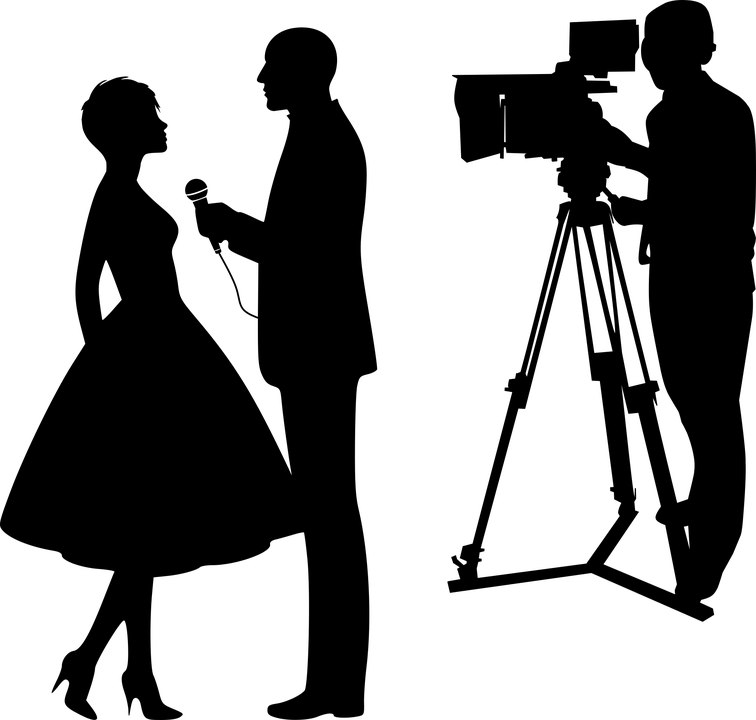
\includegraphics[width=2.90625in,height=1.93750in]{media/image16.png}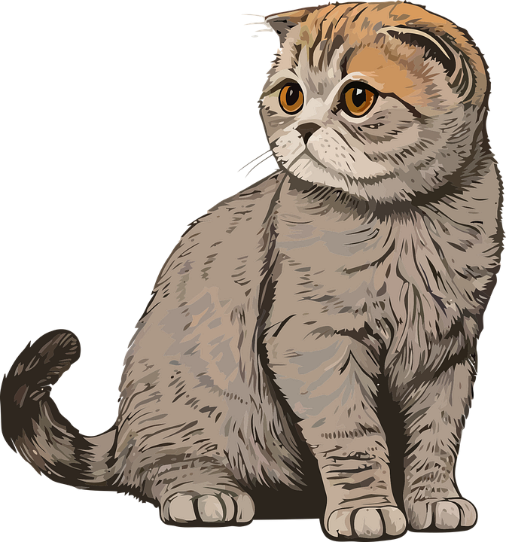
\includegraphics[width=3.08071in,height=1.93864in]{media/image17.png}

%"Morro": \emph{https://br.freepik.com/fotos-gratis/bela-vista-de-uma-pequena-cidade-nas-montanhas-durante-o-por-do-sol-no-brasil\_15695652.htm\#query=favela\&position=0\&from\_view=search\&track=sph}

%"Asfalto": \emph{https://www.pexels.com/pt-br/foto/fotografia-aerea-aerofotografia-arquitetura-tiro-com-drone-7937279/}

\num{c} Converse com os seus colegas e com seu professor sobre as referências ao
"morro" e ao "asfalto" indicadas pelo texto 2, observe as imagens e, em
seguida, escreva as diferenças percebida entre esses dois espaços.

\linhas{3}
\coment{Aqui, o professor deve guiar a discussão sobre como a diferença espacial
de habitação é reveladora da diferença étnico-racial, cultural e de
classe em uma sociedade. Podem ser apontadas como diferenças: Qualidade
dos edifícios, amplitude das ruas, arborização, entre outras.}

Vocês acham que existe uma separação de raça entre as pessoas que vivem
nos "morros" e no "asfalto" no Brasil? Discuta com seu professor e anote
os dados indicados por ele abaixo:

\begin{quote}
Porcentagem da população em morros e favelas no Brasil:

Negros: 66\%

Brancos: 34\%

Considerando a distribuição de acordo com o chefe da família, tem-se que
40,1\% dessas casas são chefiadas por homens negros, 26\% por mulheres
negras, 21,3\% por homens brancos e 11,7\% por mulheres brancas.
\end{quote}

\num{d} Segundo o texto, ao saírem dos morros e favelas para viverem nas
moradias construídas pelo Projeto Integrado Entrada da Cidade (Piec), a
desigualdade entre brancos e negros diminui?

\linhas{3}
\coment{Aqui, espera-se que o aluno volte ao texto e diga que não, uma vez que
os brancos ainda são colocados nas residências da frente e separados dos
negros, que em sua maioria vivem nas casas da parte de trás da Entrada
da Cidade.}

\colorsec{Atividade 3}

\coment{Habilidade BNCC EF05HI03: Analisar o papel das culturas e das religiões
na composição identitária dos povos antigos.

Habilidade SAEB: 12. Reconhecer os modos de comunicação próprios da
cultura oral, da imprensa, da radiodifusão, da televisão, do cinema, da
internet ou de outras tecnologias digitais de informação.}

Leia o texto a seguir e responda às questões

\coment{Recomenda-se que essa atividade seja feita em duplas ou trios.}

\begin{quote}
Durante séculos, a opinião mundial se alimentou de pensamentos
distorcidos sobre a história da África, inspirados por pensadores
europeus como Friedrich Hegel, autor da frase ``A África não possui
consciência exterior que possa resultar em universalidade''. A África
foi rotulada pelos europeus como uma terra sem história, por falta de
registros escritos, apesar da escrita ter nascido no continente.

A tradição oral sempre teve um importante papel na cultura africana. A
maioria das informações culturais, sociais e ancestrais eram
transmitidas oralmente, de uma geração em geração. Os griôs e os mais
velhos eram, e em alguns lugares continuam, sendo os responsáveis por
essas transmissões. Como dizia o escritor Amadou Hampaté Bâ, natural de
Mali ``Na África, quando morre um velho, é toda uma biblioteca que
queima''.

Desde a antiguidade, grandes fatos históricos e grandes nomes de heróis
eram imortalizados pela música. Todo povo tinha seus griôs que conheciam
sua história de cor e a passavam para seus filhos, visto que em geral,
ser griô era uma função hereditária. Até hoje, nos países do Sul do
Saara, é comum encontrar um jovem griô de vinte anos que consiga contar
a história de uma família por sete gerações através de uma canção
enquanto dedilha sua Kora. Além de ser o jornal da comunidade, a música
na África também sempre carregou lições de moral, já que ela é destinada
a todos. Por isso que muitas músicas tradicionais eram até histórias do
dia a dia (storytelling) que findavam com um ensinamento.
\end{quote}

\num{a} Segundo o texto, qual é a importância da oralidade para os povos africanos?

\linhas{3}
\coment{Espera-se que o aluno fale sobre a importância da oralidade na garantia
da perpetuação da cultura, da história e dos costumes dos povos
africanos desde a antiguidade.}

\num{b} Segundo o que você leu, o que é história oral?

\linhas{3}
\coment{Aqui espera-se que o aluno diferencie a história oral da história
escrita, entendendo ambas como igualmente relevantes. Deve-se destacar o
processo da oralidade, da comunicação direta e da passagem de
informações através de gerações.}

\num{c} Cite dois tipos de história oral presentes no texto:

\begin{enumerate}
\item \preencher \coment{Contar histórias - griô}

\item \preencher \coment{Músicas}
\end{enumerate}

A cultura escrita tem seus primórdios na escrita cuneiforme de onde hoje
se situa o Egito, no Nordeste da África. Apesar disso, segundo o autor
do texto que lemos, a África foi por muito tempo considerada um
continente sem história. Discuta com seus alunos o porquê disso e
elenque 3 argumentos que combatam essa visão:

\begin{enumerate}
\item \linhas{3}

\item \linhas{3}

\item \linhas{3}
\end{enumerate}

\coment{1. A África é um continente múltiplo, e não deve ser considerada uma só.
  Possui incontáveis povos e etnias, cuja história varia entre a origem
  da escrita pelos egípcios até as histórias orais de diversas
  comunidades.

2. Existem organizações sociais - complexas ou não - espalhadas pelo
  território. Existem funções sociais desempenhadas em famílias de
  maneira hereditária há muitas gerações, como a do Griô.

3. A cultura é extremamente rica, a exemplo das músicas tradicionais
  também passadas por gerações, além de outros exemplos de culturas
  materiais e imateriais.}

\colorsec{Treino}

\num{1}

\begin{quote}
Os dados indicam que a Covid-19 tem sido mais letal entre os negros
do que entre os brancos. Um ponto de partida essencial para debater essa
vulnerabilidade maior é reconhecer a desigualdade estrutural presente na
sociedade brasileira. Levantamento do IBGE, de 2018, mostra que 75\% dos
mais pobres no país são negros. Sabemos que um dos pressupostos para a
não contaminação pelo coronavírus é conseguir fazer o isolamento social.
Só que sabemos também que as condições para que esse isolamento ocorra
não são iguais para todos. Sabemos que a Covid desorganizou de maneira
bastante intensa a economia, o país de modo em geral, uma vez que muitas
pessoas não tinham trabalho formal, viviam na informalidade, ou com os
próprios negócios, ou com bicos e trabalhos que não eram fixos. Com a
falta de renda para se manterem em casa, as pessoas precisam sair para
trabalhar e, muitas vezes, se contaminam e morrem mais.

\fonte{Disponível em:
\emph{https://cee.fiocruz.br/?q=desigualdade-etnico-racial-no-Brasil-entrevista-Palloma-Menezes}
Acesso em: 23 fev. 2023.}
\end{quote}

Segundo o texto, a pandemia do Covid-19 foi pior para os negros do que
entre os brancos por causa da (do)

\begin{escolha}
\item localização de seus bairros residenciais.

\item diferença em suas condições financeiras.

\item cultura de higienização das mãos.

\item mudança de seus hábitos alimentares.
\end{escolha}

\coment{EF05GE02: Identificar diferenças étnico-raciais e étnico-culturais e
desigualdades sociais entre grupos em diferentes territórios.

Habilidade SAEB: 3A7: Identificar diferenças étnico-raciais e culturais
entre grupos em situações de desigualdade socioespacial.

a) Incorreta. O texto não fala sobre a região habitada pelos grupos;
b) Correta. De fato, a diferença da condição financeira dos grupos
afetou um mais do que o outro no combate à pandemia;
c) Incorreta. O texto não menciona uma diferença entre os grupos de
higienização;
d) Incorreta. O texto não fala sobre hábitos alimentares.}

\num{2}

\begin{quote}
A Ágora era o nome que se dava às praças públicas na Grécia Antiga.
Nestas praças ocorriam reuniões onde os gregos discutiam assuntos
ligados à vida da cidade. E na história do Ocidente deu origem ao
posteriormente denominado Espaço Público. A sua denominação muda, mas a
sua essência continua. Os gregos nos deram a criação das ágoras, espaços
públicos de encontros e assembleias nas cidades, exemplo maior de
expressão de lugar urbano de liberdade, quer para as intermináveis
perorações filosóficas, quer para o comércio, e até tribunais populares.
%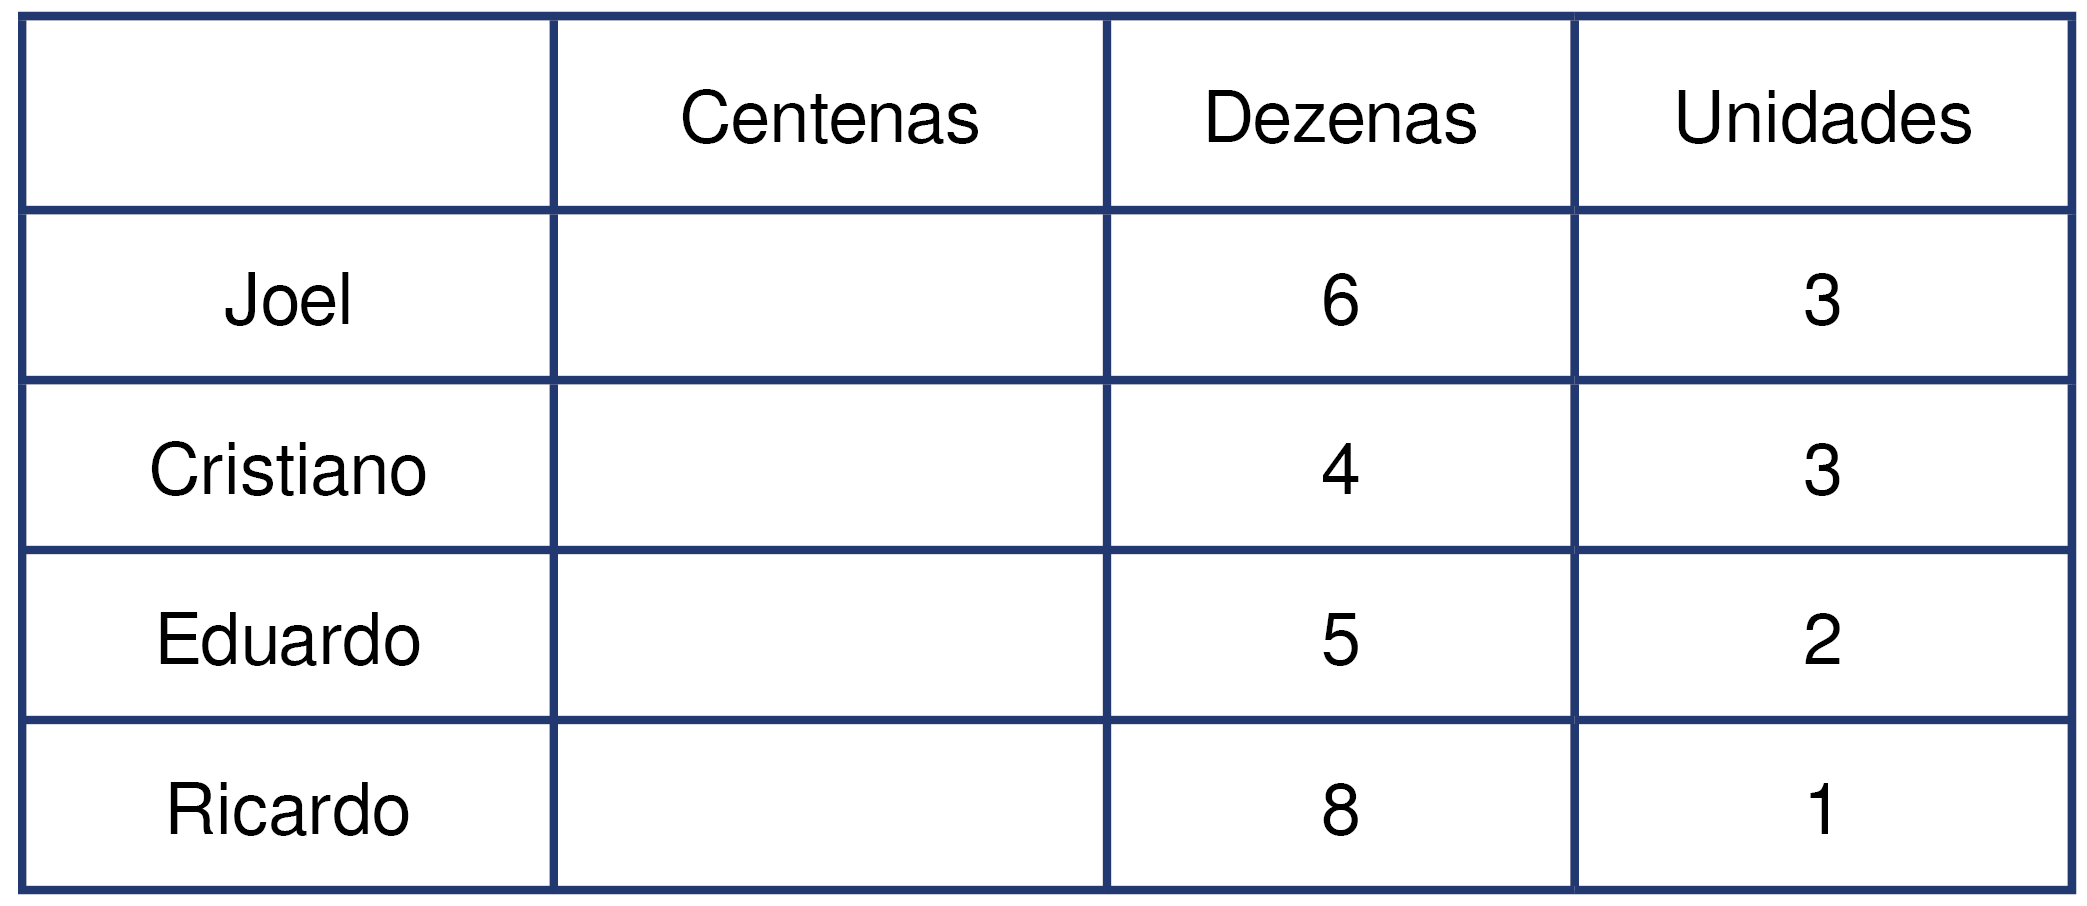
\includegraphics[width=2.91146in,height=3.62813in]{media/image18.png}
\end{quote}

Segundo o texto, a Ágora foi um importante espaço criado pela cultura
grega onde aconteciam

\begin{escolha}
\item colheitas de plantações.

\item debates entre os cidadãos.

\item rituais de cunho religioso.

\item combates entre as cidades.
\end{escolha}

\coment{EF05HI03: Analisar o papel das culturas e das religiões na composição
identitária dos povos antigos.

SAEB 3A6: Identificar diferentes tipos de apropriações e usos culturais
dos espaços públicos.

a) Incorreta. O texto não fala sobre a colheita acontecer na Ágora,
somente o comércio;
b) Correta. O texto fala sobre os debates públicos que ocorriam na
Ágora, um espaço de expressão dos considerados cidadãos na Grécia
antiga;
c) Incorreta. O texto não registra rituais acontecidos na Ágora;
d) Incorreta. O texto não fala sobre combates entre as cidades, mas da
estrutura interna de cada cidade.}

\num{3}

%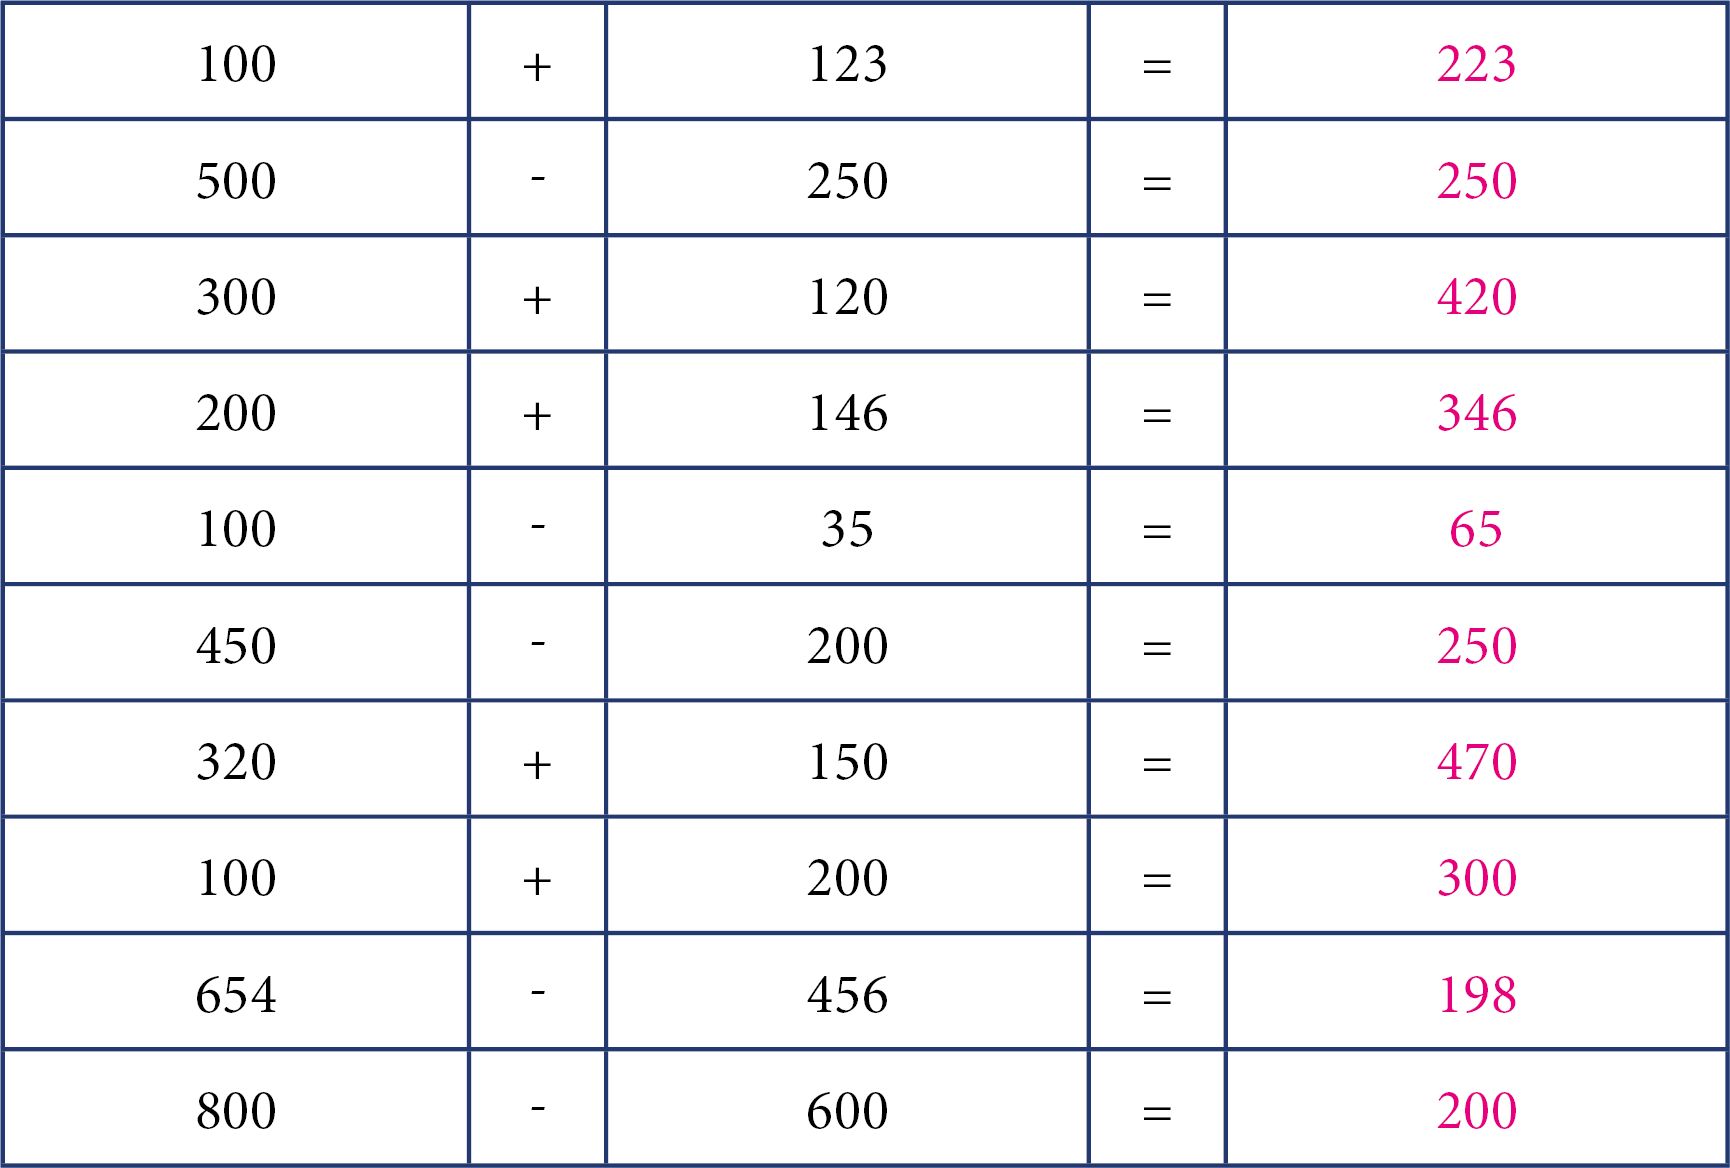
\includegraphics[width=4.84896in,height=3.22995in]{media/image19.png}
%Imagem: Reprodução IPHAN: \emph{http://portal.iphan.gov.br/pagina/detalhes/81/}

\begin{quote}
Os Saberes e Práticas Associados ao Modo de Fazer Bonecas Karajá -
patrimônio imaterial inscrito pelo Iphan, em 2012, no Livro de Registro
dos Saberes - são uma referência cultural significativa para o povo
Karajá e representam, muitas vezes, a única ou a mais importante fonte
de renda das famílias. Atualmente, a confecção dessas figuras de
cerâmica, denominadas na língua nativa de ritxòkò (na ala feminina) e/ou
ritxòò (na ala masculina), é uma atividade exclusiva das mulheres e
envolve técnicas e modos de fazer considerados tradicionais e
transmitidos de geração em geração. Mais do que objetos meramente
lúdicos, as ritxòkò são consideradas representações culturais que
comportam significados sociais profundos, reproduzindo o ordenamento
sociocultural e familiar dos Karajá.
\end{quote}

Segundo o texto, o Modo de Fazer Bonecas Karajá é importante para o povo
Karajá por dois motivos:

\begin{escolha}
\item ambiental e religioso.

\item político e alimentar.

\item escolar e comportamental.

\item financeiro e cultural.
\end{escolha}

\coment{BNCC EF05HI10: Inventariar os patrimônios materiais e imateriais da
humanidade e analisar mudanças e permanências desses patrimônios ao
longo do tempo.

SAEB: 3C2: Avaliar os critérios de definição dos marcos oficiais de
memória nas cidades.

a) Incorreta. O texto não faz menção a uma importância ambiental nem
religiosa;
b) Incorreta. O texto não aponta intenções políticas nem alimentares
relacionadas às bonecas;
c) Incorreta. O texto não fala sobre a escola nem sobre o comportamento
das mulheres que produzem as bonecas;
d) correta. O texto enfatiza a importância das bonecas para a renda das
famílias e sua relevância no contexto cultural familiar.}

\chapter{4. Poder, estado e instituições}

\coment{Habilidades da BNCC envolvidas:

EF05HI02: Identificar os mecanismos de organização do poder político com
vistas à compreensão da ideia de Estado e/ou de outras formas de
ordenação social.}

%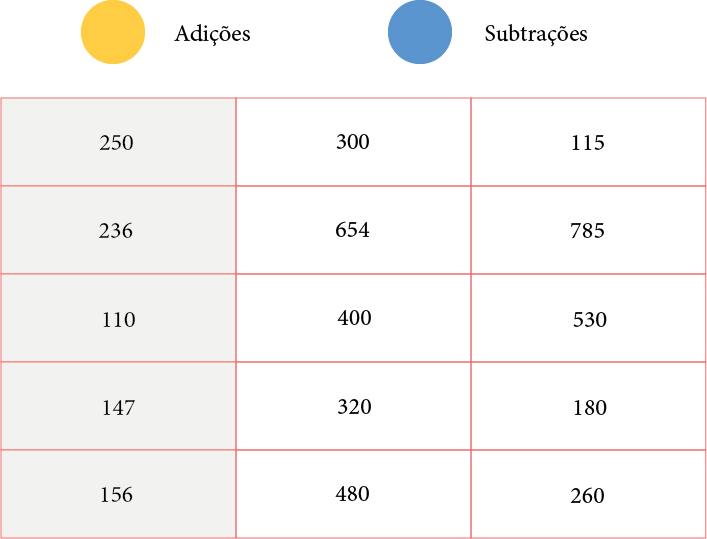
\includegraphics[width=6.26772in,height=4.18056in]{media/image20.png}
%\fonte{Disponível em: \emph{https://pixabay.com/pt/photos/globo-terra-mapa-do-mundo-mundo-1130870/} Acesso em: 23 fev. 2023.}

\conteudo{Como nossa sociedade é organizada? Quem toma conta dela? Como chegamos
nesse sistema? Desde o surgimento da raça humana tentamos nos organizar
para viver de forma mais prática e segura. Nos juntamos para nos
proteger contra os animais, depois, para cultivarmos nosso alimento, em
seguida, para crescer enquanto povo, até formarmos cidades, estados e
países. Chegamos na organização do nosso mundo de hoje a partir de nossa
história enquanto povo, enquanto humanidade.

Hoje, o mundo se divide em 6 continentes, divididos em 193 países. Cada
país tem sua própria forma de organização. O Estado brasileiro, por
exemplo, em que vivemos, tem sua Constituição, um conjunto de leis que
temos que seguir para vivermos em nossa sociedade. Ao mesmo tempo
existem organizações internacionais, como a ONU, a Organização das
Nações Unidas, que trabalham para a paz entre os países e pela garantia
dos direitos humanos a todos. Também, dentro do Brasil, temos diversas
organizações do governo ou independentes que trabalham em benefício do
bem estar social em diversas áreas: ambiental, cultural, social, entre
inúmeras outras.

Neste módulo, vamos estudar as formas de organização de nossa sociedade,
as instituições que cuidam dela e as disputas que existem entre os
vários tipos de poder social.}

\colorsec{Atividade 1}

\coment{Habilidade BNCC EF05HI02: Identificar os mecanismos de organização do
poder político com vistas à compreensão da ideia de Estado e/ou de
outras formas de ordenação social.

SAEB

4A4. Identificar os espaços que compõem a estrutura político-territorial
do Brasil cartograficamente representados.

4A3: Reconhecer as funções do Estado brasileiro nos níveis municipal,
estadual e/ou federal.}

%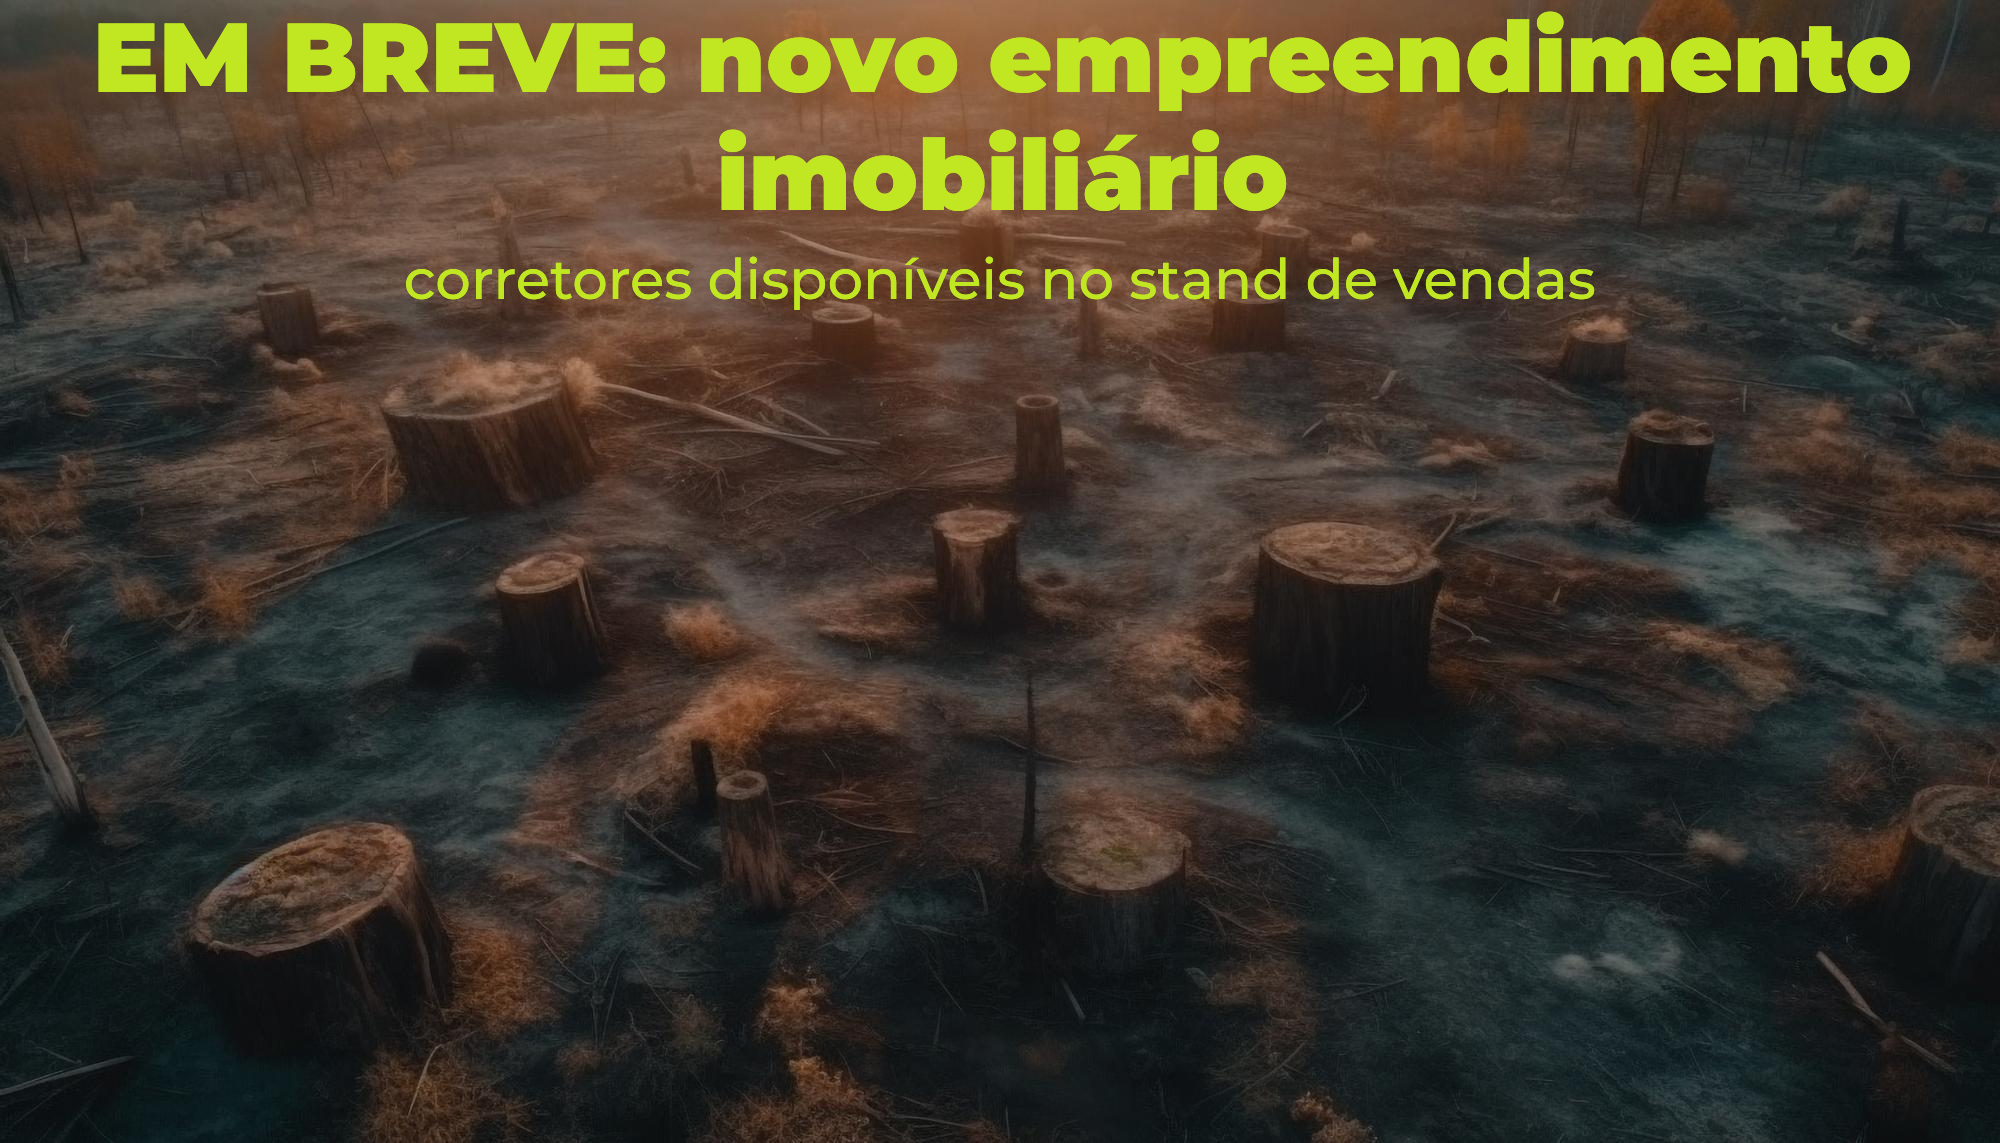
\includegraphics[width=4.39944in,height=4.39063in]{media/image21.png}

\begin{quote}
O Brasil é uma República Federativa organizada política e
administrativamente em estados, municípios e distritos. Para administrar
o país, existe uma divisão em governos: federal, estadual e municipal.

Os 26 estados brasileiros, além do Distrito Federal, compõem a República
Federativa do Brasil. Por isso, os estados são chamados de Unidades da
Federação.

A sede do governo brasileiro fica em Brasília, no Distrito Federal. É lá
que trabalha o Presidente da República.

\fonte{Disponível em:
\emph{https://educa.ibge.gov.br/criancas/brasil/nosso-territorio/19637-divisao-territorial.html}
Acesso em: 23 fev. 2023.}
\end{quote}

Observe o mapa, leia o texto, e responda as questões a seguir:

\num{a} Você sabe o que significa a divisão dos governos em Federal, Estadual e
Municipal? Com a ajuda de sua professora, preencha os governos que tomam
conta de onde você mora:

\begin{itemize}
\item Governo Federal: \preencher \coment{Brasil.}

\item Governo Estadual: \preencher \coment{preencher com o Estado em que o aluno mora.}

\item Governo Municipal: \preencher \coment{preencher com a cidade em que o aluno mora.}
\end{itemize}

\num{b} Agora, marque o estado em que você mora com um X no mapa acima.

\num{c} Você sabia que os Estados Brasileiros são divididos em 5 regiões? Com a
ajuda do seu professor e de seus colegas, pinte com 5 cores de lápis de
cor diferentes os estados que pertencem a cada região do Brasil, depois,
anote abaixo:

\begin{itemize}
\item Região Norte: \linhas{2}
\coment{Amazonas, Roraima, Amapá, Pará, Tocantins, Rondônia, Acre.}

\item Região Nordeste: \linhas{2}
\coment{Maranhão, Piauí, Ceará, Rio Grande do Norte, Pernambuco, Paraíba, Sergipe, Alagoas, Bahia.}

\item Região Centro-Oeste: \linhas{2}
\coment{Mato Grosso, Mato Grosso do Sul, Goiás, Distrito Federal.}

\item Região Sudeste: \linhas{2}
\coment{São Paulo, Rio de Janeiro, Minas Gerais e Espírito Santo.}

\item Região Sul: \linhas{1}
\coment{Paraná, Santa Catarina e Rio Grande do Sul.}

\item Em qual região você mora: \linhas{1}
\coment{Preencher com a região onde o aluno mora.}
\end{itemize}

\num{d} Você sabe para que serve essa divisão em regiões? Registre abaixo as
explicações de seu professor.

%Fazer uma região para anotações, um retângulo não muito pequeno, para que o aluno registre o que está na lousa.

\coment{Explicar aos alunos sobre a aplicabilidade das regiões: O Brasil é um
país muito grande e de Norte a Sul encontramos costumes muito
diferentes. As danças populares são típicas de cada lugar, assim como a
comida, as músicas, as atividades econômicas e às vezes a própria língua
é tão diferente que não entendemos muito bem o que dizem as pessoas de
outras regiões. Então, para melhor compreender, estudar e administrar
este nosso imenso país, o território foi dividido em cinco Grandes
Regiões: Norte, Nordeste, Sul, Sudeste e Centro-Oeste.}

\fonte{Fonte:
\emph{https://educa.ibge.gov.br/criancas/brasil/nosso-territorio/19637-divisao-territorial.html}}

\colorsec{Atividade 2}

\coment{Habilidade BNCC EF05HI02: Identificar os mecanismos de organização do
poder político com vistas à compreensão da ideia de Estado e/ou de
outras formas de ordenação social.

Habilidade SAEB: 4C4: Discutir as propostas implementadas pelo poder
público que afetam a vida das pessoas nas comunidades e cidades do país.

4A2. Identificar órgãos do Estado voltados para melhoria da qualidade de
vida das populações.}

%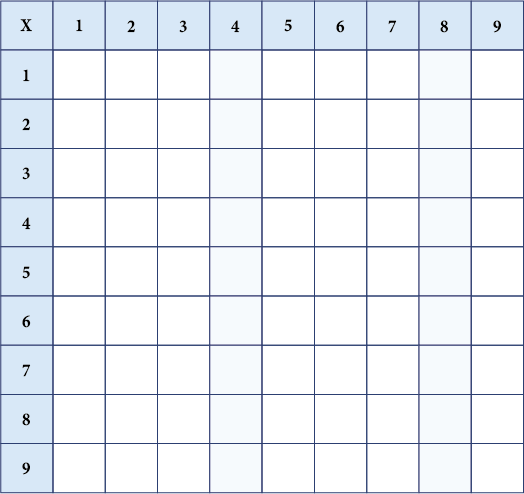
\includegraphics[width=6.26772in,height=4.18056in]{media/image22.png}
%\fonte{Disponível em: \emph{https://br.freepik.com/fotos-gratis/filhos-de-tiro-medio-deitados-juntos\_17808648.htm\#query=crian\%C3\%A7a\%20lazer\&position=25\&from\_view=search\&track=ais} Acesso em: 23 fev. 2023.}

Você sabia que é dever do Estado brasileiro proteger as crianças e
adolescentes que vivem aqui? Para isso, foi criado o ECA,
\textbf{Estatuto da Criança e do Adolescente.} Nele estão escritos
alguns direitos que devem ser garantidos pelo governo. Vamos ler 5
deles:

\begin{enumerate}
\item Direito à liberdade, ao respeito e à dignidade: O direito à
liberdade da criança compreende que tenham o direito de ir, vir e estar
em espaços públicos e comunitários, com exceção das restrições legais. O
direito de opinião e expressão, de crença, de brincar, de praticar
esportes e se divertir, de ter refúgio, auxílio e orientação, de
participar da vida familiar e comunitária sem discriminação;

\item Ser protegido da violência física ou psicológica: No artigo 17,
ainda falando do que se refere ao direito à liberdade, respeito e à
dignidade, crianças e adolescentes devem ter a integridade física, moral
e psíquica preservadas. Incluindo a preservação da imagem, identidade,
autonomia, ideias, crenças, valores, espaços e objetos pessoais. É ainda
dever de toda sociedade zelar pela dignidade das crianças e
adolescentes, protegendo de quaisquer tratamentos desumanos, violentos
ou constrangedores;

\item Direito à convivência familiar e comunitária: É direito da criança
ser educada pela sua família, excepcionalmente, por uma família adotiva.
Em ambiente que esteja garantido o seu desenvolvimento integral;

\item Direito à educação, esporte e lazer: Toda criança e adolescente têm
direito à educação, para o seu desenvolvimento pessoal, qualificação
para o trabalho e preparo para o exercício da cidadania. Este direito
deve garantir que tenham condições de acesso e permanência igualitários
na escola, que sejam respeitados pelos seus educadores, que possam
contestar critérios de avaliação, podendo se expressar e recorrer às
instâncias escolares. O ECA ainda assegura o direito de participação em
entidades estudantis e o acesso à escola pública e gratuita próxima da
sua residência;

\item Direito à profissionalização e à proteção no trabalho: É proibido
qualquer trabalho a menores de quatorze anos de idade, exceto na
condição de aprendiz. A formação técnico-profissional deve obedecer às
seguintes regras: garantia de acesso e frequência obrigatória ao ensino
regular, atividade compatível com desenvolvimento do adolescente e o
horário especial para o exercício do trabalho.
\end{enumerate}

\fonte{Disponível em:
\emph{https://www.saopaulo.sp.leg.br/blog/mes-das-criancas-conheca-5-direitos-de-criancas-e-adolescentes/\#:\textasciitilde{}:text=Garantir\%20que\%20todas\%20as\%20crian\%C3\%A7as,Poder\%20P\%C3\%BAblico\%2C\%20mas\%20de\%20toda}
Acesso em: 23 fev. 2023}

\num{a} Você conhecia todos esses direitos? Tem algum deles que você ache mais
importante? Existe algum direito fundamental que você acrescentaria a
esses 5 direitos? Converse com os colegas e anote suas ideias abaixo:

\linhas{4}
\coment{Espera-se que o aluno reflita sobre os direitos lidos. Também, que ele
entenda suas importâncias e tenha um pensamento crítico sobre essa
questão, além de propositivo, ao acrescentar algo que ele acredita que
falte no texto acima.}

\num{b} Na sua opinião, quem é responsável pela sua educação e pelo seu
bem-estar? Discuta com seus colegas.

\linhas{3}
\coment{Espera-se que o aluno fale sobre a família, a escola e o governo. Cabe
ao professor guiar o debate, e lembrar de todas as instâncias
responsáveis por cuidar dos alunos.}

\num{c} Você sabia que existe uma lei que responde a esta questão? Copie da
lousa essa lei no retângulo abaixo:

%Inserir retângulo que caiba a lei escrita.

\coment{Art. 227. É dever da família, da sociedade e do Estado assegurar à
criança e ao adolescente, com absoluta prioridade, o direito à vida, à
saúde, à alimentação, à educação, ao lazer, à profissionalização, à
cultura, à dignidade, ao respeito, à liberdade e à convivência familiar
e comunitária, além de colocá-los a salvo de toda forma de negligência,
discriminação, exploração, violência, crueldade e opressão.}

\num{d} Você sabia da existência do Estatuto da Criança e do Adolescente? Porque
você acha que ele é importante em nossa sociedade? Discuta com o
professor e seus colegas e escreva abaixo.

\linhas{3}
\coment{Falar sobre a responsabilidade do Poder Público, e não só da família, de
proteger as crianças. Discutir o conceito de direito: o que é? quem
trabalha para que ele seja garantido? Falar sobre a importância da
existência de um órgão do governo que tenha como objetivo criar
políticas públicas em prol das crianças e adolescentes.}

\num{e} Você sabe até quantos anos uma pessoa é considerada criança pelo ECA? E
adolescente? Complete com a ajuda do professor:

\begin{itemize}
\item Criança: De \preencher até \preencher anos de idade. \coment{0 até 12}

\item Adolescente: Entre \preencher e \preencher anos de idade. \coment{12 até 18}
\end{itemize}

\colorsec{Atividade 3}

\coment{Habilidade BNCC EF05HI02: Identificar os mecanismos de organização do
poder político com vistas à compreensão da ideia de Estado e/ou de
outras formas de ordenação social.

Habilidade SAEB:

4B1: Compreender as regras de convívio em diferentes espaços (sala de
aula, escola etc.).

4C1: Propor regras de convívio em espaços marcados por desorganização e
conflitos.}

\conteudo{Agora já sabemos quem são os responsáveis por cuidar das crianças e
adolescentes. Os pais, a família, a escola, e o estado tem deveres sobre
vocês.

Mas e as crianças e adolescentes, quais são seus deveres na comunidade?

Nessa atividade falaremos sobre as regras de convivência na escola.

Recomenda-se que as atividades sejam feitas em duplas ou grupos, para
que não se torne extremamente séria ou acusativa. O objetivo é que os
alunos discutam sobre as regras de maneira leve e natural.}

Vamos começar lendo uma parte dessa reportagem de 2018:

\begin{quote}
\textbf{Cotidiano: a importância das normas de convivência para o bem-estar na escola}

Quando a criança aprende a respeitar o direito do outro, entra em
contato com o conceito de ética logo na infância.

Conviver é um exercício diário de cidadania. Viver em sociedade é, acima
de tudo, uma necessidade humana. Torna-se simples quando se depende uns
dos outros para viver melhor. Esse exercício social se inclina,
principalmente, ao respeito, às diferenças e ao ato de obedecer às
regras de conduta moral e ética. Para as crianças, em especial, as
normas de relacionamento com o meio são mais bem exercidas na escola,
onde o ato de dividir o mesmo espaço é mais intenso.

\fonte{Disponível em:
\emph{https://g1.globo.com/sao-paulo/sorocaba-jundiai/especial-publicitario/objetivo-sorocaba/conduzindo-o-melhor-de-voce/noticia/cotidiano-a-importancia-das-normas-de-convivencia-para-o-bem-estar-na-escola.ghtml}
Acesso em: 23 fev. 2023.}
\end{quote}

\num{a} Vamos começar lembrando algumas \textbf{regras gerais} que temos em
nossa escola. Com a ajuda dos colegas, escreva abaixo 3 delas:

\begin{enumerate}
\item \linhas{1}

\item \linhas{1}

\item \linhas{1}
\end{enumerate}

\coment{Aqui, cabe à professora guiar a discussão dos alunos e elencar com eles
as principais regras da escola. Exemplos: chegar no horário, cuidar do
ambiente escolar, usar uniforme, etc.}

\num{b} Agora, vamos falar das regras que temos que cumprir dentro da sala de
aula:

\begin{enumerate}
\item \linhas{1}

\item \linhas{1}

\item \linhas{1}

\item \linhas{1}

\item \linhas{1}
\end{enumerate}

\coment{Aqui, cabe à professora guiar a discussão dos alunos e elencar com eles
as principais regras a serem cumpridas dentro da sala de aula. Exemplos:
obedecer ao professor, não conversar durante a explicação, sentar no
lugar correto, anotar a matéria no caderno, etc.}

\num{c} Você sabe porque as regras são importantes?

\linhas{3}

\coment{Aqui, a professora deve guiar o aluno a entender que, da mesma forma que
cabe a escola, a família e o governo tem o dever de proteger os alunos,
os alunos também tem deveres dentro da sociedade, sendo o principal
deles permitir que a educação na escola aconteça da forma mais leve e
fácil. Falar também sobre a organização e sobre a importância dela no
futuro dos alunos.}

\colorsec{Treino}

\num{1}

\begin{quote}
Segundo a nossa Constituição, a República Federativa do Brasil é
formada pelos Estados, Municípios e pelo Distrito Federal, que se aliam
numa união indissolúvel para a formação de um Estado Federal ou
Federação. Por isso é que a Constituição, em seu primeiro artigo,
estabelece que a organização político-administrativa da República
Federativa do Brasil abrange os Estados, o Distrito Federal, os
Municípios e a União - com U maiúsculo - pessoa jurídica que resultou
daquela união indissolúvel, que representa a Federação.

\fonte{Disponível em: \emph{https://dspace.almg.gov.br/} Acesso em: 23 fev. 2023.}
\end{quote}

Um exemplo de município é:

\begin{escolha}
\item o bairro Cidade Nova na cidade de Manaus.

\item o estado de Minas Gerais no Sudeste.

\item a cidade de Campinas em São Paulo.

\item a região Nordeste do Brasil.
\end{escolha}

\coment{Habilidade BNCC EF05HI02: Identificar os mecanismos de organização do
poder político com vistas à compreensão da ideia de Estado e/ou de
outras formas de ordenação social.

Habilidade SAEB:

4A1: Identificar mecanismos da organização estatal nas diferentes
sociedades contemporâneas.

4A3: Reconhecer as funções do Estado brasileiro nos níveis municipal,
estadual e/ou federal.

a) Incorreta. Um bairro está dentro de um município;
b) Incorreta. Um estado tem vários municípios dentro dele;
c) Correta. Os municípios equivalem às cidades, assim, Campinas é um
município;
d) Incorreta. Uma região é composta por vários estados, que tem vários
municípios.}

\num{2}

\begin{quote}
As terras hoje chamadas Brasil têm muitos nomes, atribuídos pelos
povos originários, como Pindorama e Yvy Rupa. Já o continente que hoje
vemos nos livros de história como América é conhecido também por muitas
nomeações: Abya Ayla, Tawantinsuyu, Anáhuac, dados respectivamente pelos
povos Kuna, Inca e Asteca. Com os nomes, aprendemos a importância das
coisas: dar um nome a uma região, a uma pessoa ou a um povo é um ato de
identificar os lugares e os seres. Você conhece a palavra identidade?
Pois é, essa expressão tem tudo a ver com identificar o mundo: as
identidades são o que tornam as pessoas -- e os grupos de pessoas-
únicas, assim como os locais que conhecemos e os povos que vivem nesses
lugares.

\fonte{Disponível em: \emph{https://nheepora.mlp.org.br/} Acesso em: 23 fev 2023.}
\end{quote}

Segundo o texto, ao dar nome a um território estamos

\begin{escolha}
\item protegendo suas florestas.

\item expressando suas características.

\item medindo seu valor econômico.

\item julgando sua beleza natural.
\end{escolha}

\coment{Habilidade BNCC EF05HI02: Identificar os mecanismos de organização do
poder político com vistas à compreensão da ideia de Estado e/ou de
outras formas de ordenação social.

Habilidade SAEB: 4C2. Discutir os elementos políticos e sociais ligados
às políticas de reconhecimento e gestão do patrimônio.

a) Incorreta. Não há indícios no texto sobre a relação da nomeação com
proteção;
b) Correta. Ao nomear um território, estamos expressando as
características identitárias de seu povo;
c) Incorreta. Não há relação no texto entre nome e valor econômico;
d) Incorreta. Não há relação no texto entre nomeação e beleza natural.}

\num{3}

\begin{quote}
\textbf{Estatuto da Criança e do Adolescente Lei nº 8.069, de 13 de julho de 1990}

Art. 7º A criança e o adolescente têm direito à proteção à vida e à
saúde, mediante a efetivação de políticas sociais públicas que permitam
o nascimento e o desenvolvimento sadio e harmonioso, em condições dignas
de existência.
\end{quote}

Quem é responsável pela criação de políticas sociais públicas de que
fala o texto?

\begin{escolha}
\item o professor.

\item a escola.

\item a família.

\item o estado.
\end{escolha}

\coment{Habilidade BNCC EF05HI02: Identificar os mecanismos de organização do
poder político com vistas à compreensão da ideia de Estado e/ou de
outras formas de ordenação social.

Habilidade SAEB: 4B3. Diferenciar os papéis e responsabilidades dos
sujeitos frente à família, à escola e à comunidade.

a) Incorreta. Não é o professor, mas o estado o responsável pela criação
de políticas públicas;
b) Incorreta. O estado é o responsável pela criação de políticas
públicas, cabe a escola segui-las;
c) Incorreta. Não é a família, mas o estado o responsável pela criação
de políticas públicas;
d) Correta. O estado e o poder público são responsáveis pela criação de
políticas sociais.}

\chapter{5. Cidadania, direitos humanos e movimentos sociais}

\coment{Habilidades da BNCC envolvidas:

EF05HI04: Associar a noção de cidadania com os princípios de respeito à
diversidade, à pluralidade e aos direitos humanos.

EF05HI05: Associar o conceito de cidadania à conquista de direitos dos
povos e das sociedades, compreendendo-o como conquista histórica.}

\conteudo{Você é um cidadão brasileiro. Mas você sabe o que isso significa?
Significa que a partir do momento em que você nasce no Brasil, você
passa a fazer parte de nossa República, e tem direitos fundamentais e
deveres dentro do território nacional. Alguns desses direitos nós já
aprendemos no Módulo 4, quando estudamos o Estatuto da Criança e do
Adolescente(ECA). Porém, não são só as crianças e adolescentes que tem o
direito à vida, à liberdade, à igualdade, à segurança e à propriedade.
São todos os cidadãos brasileiros.

%
\includegraphics[width=3.23438in,height=3.22079in]{media/image23.png}

Porém, não são só as pessoas que nascem no Brasil que tem seus direitos
garantidos. Ao longo da história foi construída a ideia de
\textbf{direitos humanos}, que são direitos que \textbf{todos os seres
humanos}, em todos os países, independente do que acontece no lugar em
que eles nasceram, devem ter. Quem trabalha para garantir esses direitos
são Órgãos internacionais, como a ONU, a Organização das Nações Unidas.

Nesse módulo vamos trabalhar o conceito de cidadania e entender nossos
direitos enquanto cidadãos brasileiros e cidadãos do mundo. Também,
vamos ver como podemos lutar para que os nossos direitos básicos sejam
garantidos, para que todos possam viver de maneira feliz e digna.

\fonte{Disponível em:
\emph{https://br.freepik.com/vetores-gratis/pare-o-conceito-de-ilustracao-de-racismo\_8944994.htm\#page=2\&query=direitos\%20humanos\&position=36\&from\_view=search\&track=ais}
Acesso em: 23 fev. 2023.}}

\colorsec{Atividade 1: Direitos humanos}

\coment{Habilidade BNCC EF05HI04: Associar a noção de cidadania com os
princípios de respeito à diversidade, à pluralidade e aos direitos
humanos.

Habilidade SAEB 5B6: Relacionar a noção de cidadania com os princípios
de respeito à diversidade, à pluralidade e aos direitos humanos.

5A3. Reconhecer formas de atuação condizentes e não condizentes com os
direitos humanos nos espaços público e doméstico.}

Vamos ler uma parte da \textbf{Declaração Universal dos Direitos Humanos}, de 1948

\begin{quote}
Considerando que os povos das Nações Unidas reafirmaram, na Carta, sua
fé nos direitos fundamentais do ser humano, na dignidade e no valor da
pessoa humana e na igualdade de direitos do homem e da mulher e que
decidiram promover o progresso social e melhores condições de vida em
uma liberdade mais ampla,

Agora portanto a Assembléia Geral proclama a presente Declaração
Universal dos Direitos Humanos como o ideal comum a ser atingido por
todos os povos e todas as nações, com o objetivo de que cada indivíduo e
cada órgão da sociedade tendo sempre em mente esta Declaração,
esforce-se, por meio do ensino e da educação, por promover o respeito a
esses direitos e liberdades, e, pela adoção de medidas progressivas de
caráter nacional e internacional, por assegurar o seu reconhecimento e a
sua observância universais e efetivos, tanto entre os povos dos próprios
Países-Membros quanto entre os povos dos territórios sob sua jurisdição.

\textbf{Artigo 1}

Todos os seres humanos nascem livres e iguais em dignidade e direitos.
São dotados de razão e consciência e devem agir em relação uns aos
outros com espírito de fraternidade.

\textbf{Artigo 2}

1. Todo ser humano tem capacidade para gozar os direitos e as liberdades
estabelecidos nesta Declaração, sem distinção de qualquer espécie, seja
de raça, cor, sexo, língua, religião, opinião política ou de outra
natureza, origem nacional ou social, riqueza, nascimento, ou qualquer
outra condição.

2. Não será também feita nenhuma distinção fundada na condição política,
jurídica ou internacional do país ou território a que pertença uma
pessoa, quer se trate de um território independente, sob tutela, sem
governo próprio, quer sujeito a qualquer outra limitação de soberania.

\textbf{Artigo 3}

Todo ser humano tem direito à vida, à liberdade e à segurança pessoal.

\fonte{Disponível em:
\emph{https://www.unicef.org/brazil/declaracao-universal-dos-direitos-humanos}
Acesso em: 23 fev. 2023}
\end{quote}

\num{a} Agora, discuta com seus colegas e marque com um X as situações abaixo
que você considera que vão \textbf{contra} os direitos humanos.

\begin{boxlist}
\item Ameaçar a vida de alguém.

\item Torturar ou castigar alguém usando violência.

\item Garantir moradia a todos.

\item Trabalho escravo e forçado.

\item Tratar todos de maneira igual.

\item Ser condenado de maneira injusta.

\item Dar bom salário e boas condições de trabalho.

\item Tratar alguém diferente por causa de sua cor de pele.
\end{boxlist}

\num{2} E se você trabalhasse em um organismo internacional e tivesse que
resolver algum dos problemas citados acima? O que você faria?

\coment{Divida a sala em 6 grupos e atribua a cada um deles uma das situações
abaixo. Peça que eles pensem em soluções simples e diretas para os
problemas de ameaça aos direitos humanos. A ideia é que não seja algo
extremamente elaborado, mas que eles

Sugestões:

Grupos 1 e 2: Trabalho escravo e forçado.

Grupos 3 e 4: Torturar ou castigar alguém usando violência.

Grupos 5 e 6: Tratar alguém diferente por causa de sua cor de pele.}

\begin{itemize}
\item Nome: \coment{Nome do Aluno}

\item Ano: \coment{Ano do Aluno}

\item Nome da Organização: \coment{Pedir aos alunos que dêem um nome para o grupo. Ex:
Defensores dos direitos humanos.}

\item Integrantes: \coment{Completar com os outros colegas do grupo.}

\item Problema: \coment{Colocar o problema atribuído ao grupo.}

\item Propostas: \coment{Preencher com as propostas do grupo.}
\end{itemize}

%Aqui, deixar um espaço maior para ser preenchido, talvez um retângulo.

\colorsec{Atividade 2: Lutas e conquistas}

\coment{Habilidade BNCC EF05HI05: Associar o conceito de cidadania à conquista
de direitos dos povos e das sociedades, compreendendo-o como conquista
histórica.

Habilidade SAEB: 5B7: Relacionar a conquista de direitos à construção do
conceito ou ao exercício da cidadania.}

Você sabia que até o ano de 1932 as mulheres não podiam votar no Brasil?

Vamos ler um texto sobre como aconteceu essa conquista:

%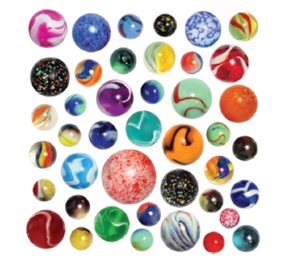
\includegraphics[width=4.04688in,height=4.03608in]{media/image24.png}
\begin{quote}
A conquista do voto feminino no Brasil se deu em 1932, resultado de um
processo de lutas, avanços e recuos que se iniciou por volta de 1910.

Em 1910 (...), a professora carioca Leolinda de Figueiredo Daltro
(1860-1935), em protesto à recusa de seu pedido de alistamento
eleitoral, fundou o Partido Republicano Feminino. Considerado o primeiro
partido político feminino do país, defendia o direito ao voto para as
mulheres e a abertura dos cargos públicos a todos os brasileiros.

Durante os trabalhos da primeira Assembleia Constituinte da República,
alguns parlamentares apresentaram propostas concretas de extensão do
direito de voto às mulheres. Lopes Trovão apresentou uma emenda que foi
(...) rejeitada e a Constituição da República dos Estados Unidos do
Brasil de 1891 não contemplou as mulheres com esse direito de cidadania.
O texto da Constituição de 1891, porém, não vedava expressamente o
direito de as mulheres votarem. Valendo-se disso, a estudante de direito
Maria Ernestina, conhecida como Mietta Santiago, (...) obteve sentença
que lhe permitiu votar em si mesma para um mandato de deputada federal.

Em 1932, foi promulgado o novo Código Eleitoral, cuja comissão de
redação contou com a participação de Bertha Lutz. Estava assegurada a
cidadania política às mulheres brasileiras, embora sem a exigência da
obrigatoriedade do alistamento eleitoral e do voto. Os arts. 2º e 21 do
novo Código Eleitoral continham os seguintes textos:

Art. 2º. É eleitor o cidadão maior de 21 anos, sem distinção de sexo,
alistado na forma deste Código. (...)

Art. 121. Os homens maiores de sessenta anos e as mulheres de qualquer
idade podem isentar-se de qualquer obrigação ou serviço de natureza
eleitoral.

Posteriormente, a Constituição da República dos Estados Unidos do Brasil
de 1934 ratificou o direito constitucional de voto das mulheres.

\fonte{Disponível em:
\emph{https://www.camara.leg.br/internet/agencia/infograficos-html5/a-conquista-do-voto-feminino/analise.html}
Acesso em: 23 fev 2023. (Adaptado)}
\end{quote}

\num{a} Você sabia que o voto é um direito de todos os cidadãos? Escreva qual
você acha que é a importância dele para nós:

\linhas{3}

\coment{Aqui o professor deve guiar a discussão, primeiramente, sobre o que
significa votar: eleger uma pessoa para nos representar nas decisões
políticas e sociais de nosso país. Em segundo lugar, deve-se pensar
sobre o voto como uma escolha e expressão dos pensamentos de cada
indivíduo. Por fim, o professor deve enfatizar que o voto foi uma
conquista dos cidadãos ao longo da história, e que devemos utilizar esse
mecanismo em nosso favor.}

\num{b} Apesar de no Brasil as mulheres poderem votar desde 1932, em alguns
países isso aconteceu ainda mais tarde. Na Árábia Saudita, por exemplo,
as mulheres só podem votar desde o ano de 2011. Porque você acha que
demorou tanto tempo para as mulheres conquistarem a possibilidade de
votar no Brasil e no mundo?

\linhas{3}
\coment{Aqui, o professor deve guiar de maneira cautelosa o debate. Falar sobre
o preconceito contra as mulheres na história da humanidade e que, apesar
de hoje, em nossa sociedade, entendermos os homens e as mulheres como
iguais, nem sempre foi assim.}

\num{c} O voto pode ser considerado uma conquista das mulheres? Cite as
personagens que o texto aponta como importantes nesse processo e o que
elas fizeram para lutar a favor dos direitos das mulheres enquanto
cidadãs:

\linhas{3}
\coment{Sim. Aqui, o professor deve guiar o aluno a entender os conceitos de
luta e conquista de direitos humanos, sociais e políticos.

Personagens:\\
Leolinda de Figueiredo Daltro (1860-1935), em protesto à recusa de seu
pedido de alistamento eleitoral, fundou o Partido Republicano Feminino.\\
Mietta Santiago, (...) obteve sentença que lhe permitiu votar em si
mesma para um mandato de deputada federal.\\
Bertha Lutz, ajudou a escrever o Código eleitoral de 1932.}

\colorsec{Atividade 3: A cidadania nas redes sociais}

\coment{EF05HI04: Associar a noção de cidadania com os princípios de respeito à
diversidade, à pluralidade e aos direitos humanos

Habilidade SAEB: 5C4: Discutir a influência dos canais de participação
social (em áreas como meio ambiente, mobilidade, moradia, direito à
cidade) na comunidade e na busca de soluções para a melhoria da
qualidade de vida.

5C3: Avaliar as transformações ocorridas nos meios de comunicação e seus
significados para os diferentes grupos ou estratos sociais}

%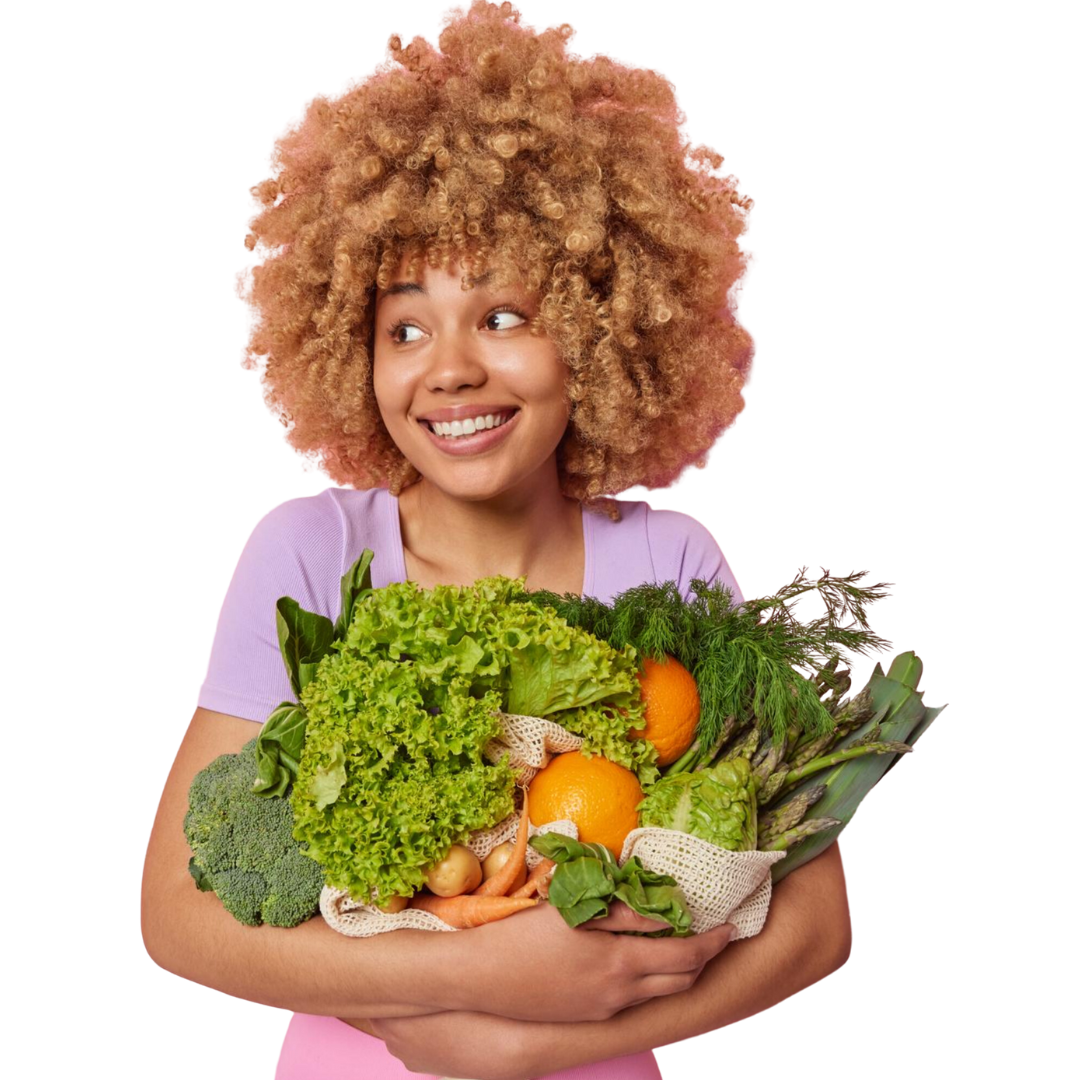
\includegraphics[width=5.58854in,height=3.72260in]{media/image25.png}
%\fonte{Disponível em: \emph{https://br.freepik.com/fotos-gratis/pile-of-3d-twitter-logos\_1191372.htm\#query=twitter\&position=9\&from\_view=search\&track=sph} Acesso em: 23 fev. 2023.}

\begin{quote}
\textbf{Desaparecimento do Twitter seria má notícia para ativistas
políticos, dizem analistas }

Existem outras plataformas, mas o Twitter "é claramente muito influente
ao fazer com que a mídia e os líderes prestem atenção no que acontece no
mundo", disse à AFP Mahsa Alimardani, pesquisadora da organização de
defesa da liberdade de expressão Artigo 19.

--- Nesse sentido, é uma plataforma única e muito especial ---
acrescenta. --- {[}No Irã{]} é o único acesso real a vozes e eventos, na
ausência de correspondentes estrangeiros e jornalistas independentes que
possam informar sobre o que está acontecendo.

O Twitter tem desempenhado um papel fundamental na promoção de fenômenos
sociais como o \#Metoo (eu também), para denunciar a violência contra a
mulher, ou o \#Blacklivesmatter (Vidas negras importam), para denunciar
a violência policial contra negros nos Estados Unidos.

--- As características do Twitter permitem dar uma identidade aos
movimentos de protesto, criar um sentimento comum ao compartilhar memes
e hashtags --- explicou à AFP Marcus

\fonte{Disponível em:
\emph{https://oglobo.globo.com/mundo/noticia/2022/11/desaparecimento-do-twitter-seria-ma-noticia-para-ativistas-politicos-dizem-analistas.ghtml}
Acesso em: 23 fev. 2023}
\end{quote}

\num{a} Você sabe o que é uma rede social? Cite as que você conhece.

\linhas{2}
\coment{Falar sobre redes sociais como comunidades online onde ocorrem trocas
entre pessoas. Os alunos ficam livres para citar as que conhecem:
Instagram, Facebook, twitter, tiktok, etc.}

\num{b} Você acha que as redes sociais podem ajudar na luta por nossos direitos? Como?

\linhas{2}
\coment{Aqui, volte ao texto e descreva como ele narra a importância do twitter
como plataforma de visibilidade, debate e troca entre as pessoas.}

\num{c} Cite dois exemplos de situações que o texto mostra que o twitter ajudou
em movimentos sociais:

\begin{enumerate}
\item \linhas{1} \coment{Movimento vidas negras importam, para denunciar a violência policial
  contra a comunidade negra.}

\item \linhas{1} \coment{Eu também, de combate à violência contra a mulher.}
\end{enumerate}

\num{d} Seu post na rede social:

Se você pudesse acabar com qualquer injustiça no mundo, qual seria?
Escreva ou desenhe um post que você faria para ajudar nessa luta:

%Deixar espaço retangular grande para que os alunos façam o post.

\coment{Aqui, o aluno deve exercitar sua criatividade.}

\colorsec{Treino}

\num{1}

%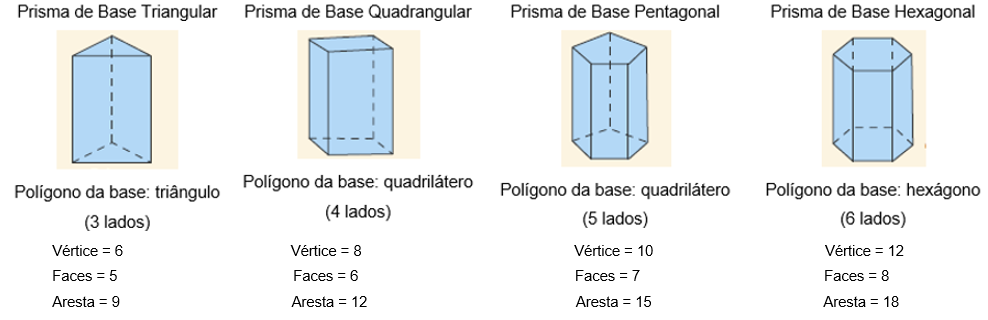
\includegraphics[width=6.26772in,height=2.44444in]{media/image26.png}

\begin{quote}
\textbf{Vital, qual é a importância do voto?}

Votar quer dizer declarar a nossa escolha entre duas ou mais opções.
Falando assim, parece uma coisa simples, né? Mas, quando se trata de
eleições, votar é um assunto muito sério. É escolher entre as propostas
de futuro que a gente quer para a nossa comunidade, o nosso estado, o
nosso país!

\noindent\textbf{Nossa, voto é assunto sério, mesmo!}

Com certeza! Quando o eleitor vota em um representante -- deputado,
senador, governador, presidente -, é como se dissesse: ``estou confiando
em você para falar em meu nome e tomar por mim todas as decisões
importantes do País''. Não dá para fazer essa escolha sem pensar bem,
né?

\fonte{Disponível em:
\emph{https://plenarinho.leg.br/index.php/2022/09/turma-explica-eleicoes-qual-importancia-voto/}
plenarinho.leg.br - Câmara dos Deputados Acesso em: 23 fev. 2023.}
\end{quote}

Segundo Vital, ao votar estamos

\begin{escolha}
\item escolhendo o futuro do país.

\item decidindo nossa profissão.

\item disfarçando nossos erros.

\item cuidando da saúde do nosso corpo.
\end{escolha}

\coment{Habilidade BNCC EF05HI04: Associar a noção de cidadania com os
princípios de respeito à diversidade, à pluralidade e aos direitos
humanos.

Habilidade SAEB: 5A1. Identificar práticas e papéis sociais que as
pessoas exercem em diferentes comunidades.

a) Correta. Vital fala que estamos escolhendo quem vai tomar as decisões
do futuro do nosso país por nós;
b) Incorreta. Vital não fala sobre decidir sua profissão;
c) Incorreta. Vital não fala que o voto serve para disfarçar nossos
erros;
d) Incorreta. Vital não coloca o voto como diretamente relacionado com a
saúde corporal.}

\num{2}

\begin{quote}
\textbf{Crianças indígenas defendem demarcação de terra e autonomia
sobre territórios}

Brincar perto da natureza, ter uma casa para morar, manter os costumes
da sua família, ir para a escola e viver em segurança são direitos de
todas as crianças, mas em algumas terras indígenas eles estão ameaçados.
Isso ocorre porque estes territórios são invadidos por pessoas e
empresas que querem explorar a natureza e expulsar os indígenas. A luta
tem conquistado cada vez mais apoiadores graças a muitos jovens
indígenas que se tornaram influencers e usam o youtube, o instagram e
outras redes sociais para falar sobre sua cultura, suas reivindicações e
também sobre música, literatura, jogos online e diversos outros
assuntos.

\fonte{Disponível em:
\emph{https://www.brasildefato.com.br/2022/04/20/criancas-indigenas-defendem-demarcacao-de-terra-e-autonomia-sobre-territorios}
Acesso em: 23 fev. 2023.}
\end{quote}

Segundo o texto os jovens indígenas usam as redes sociais para

\begin{escolha}
\item ganhar dinheiro com publicações pagas.

\item prejudicar aqueles que tentam os ameaçar.

\item mostrar aos outros sua cultura e suas lutas.

\item pedirem pela separação com o Brasil.
\end{escolha}

\coment{Habilidade BNCC EF05HI05: Associar o conceito de cidadania à conquista
de direitos dos povos e das sociedades, compreendendo-o como conquista
histórica.

Habilidade SAEB: 5B5. Compreender as diferentes manifestações sociais de
usufruto do espaço público.

5C3: Avaliar as transformações ocorridas nos meios de comunicação e seus
significados para os diferentes grupos ou estratos sociais.

a) Incorreta. O texto não fala sobre a intenção de ganhar dinheiro;
b) Incorreta. O texto não fala sobre tentativa de prejudicar o outro;
c) Correta. De fato, o texto fala que os jovens utilizam as redes para
dar visibilidade a suas lutas e a sua cultura;
d) Incorreta. Não há menção a um pedido de separação ao território
brasileiro.}

\num{3}

%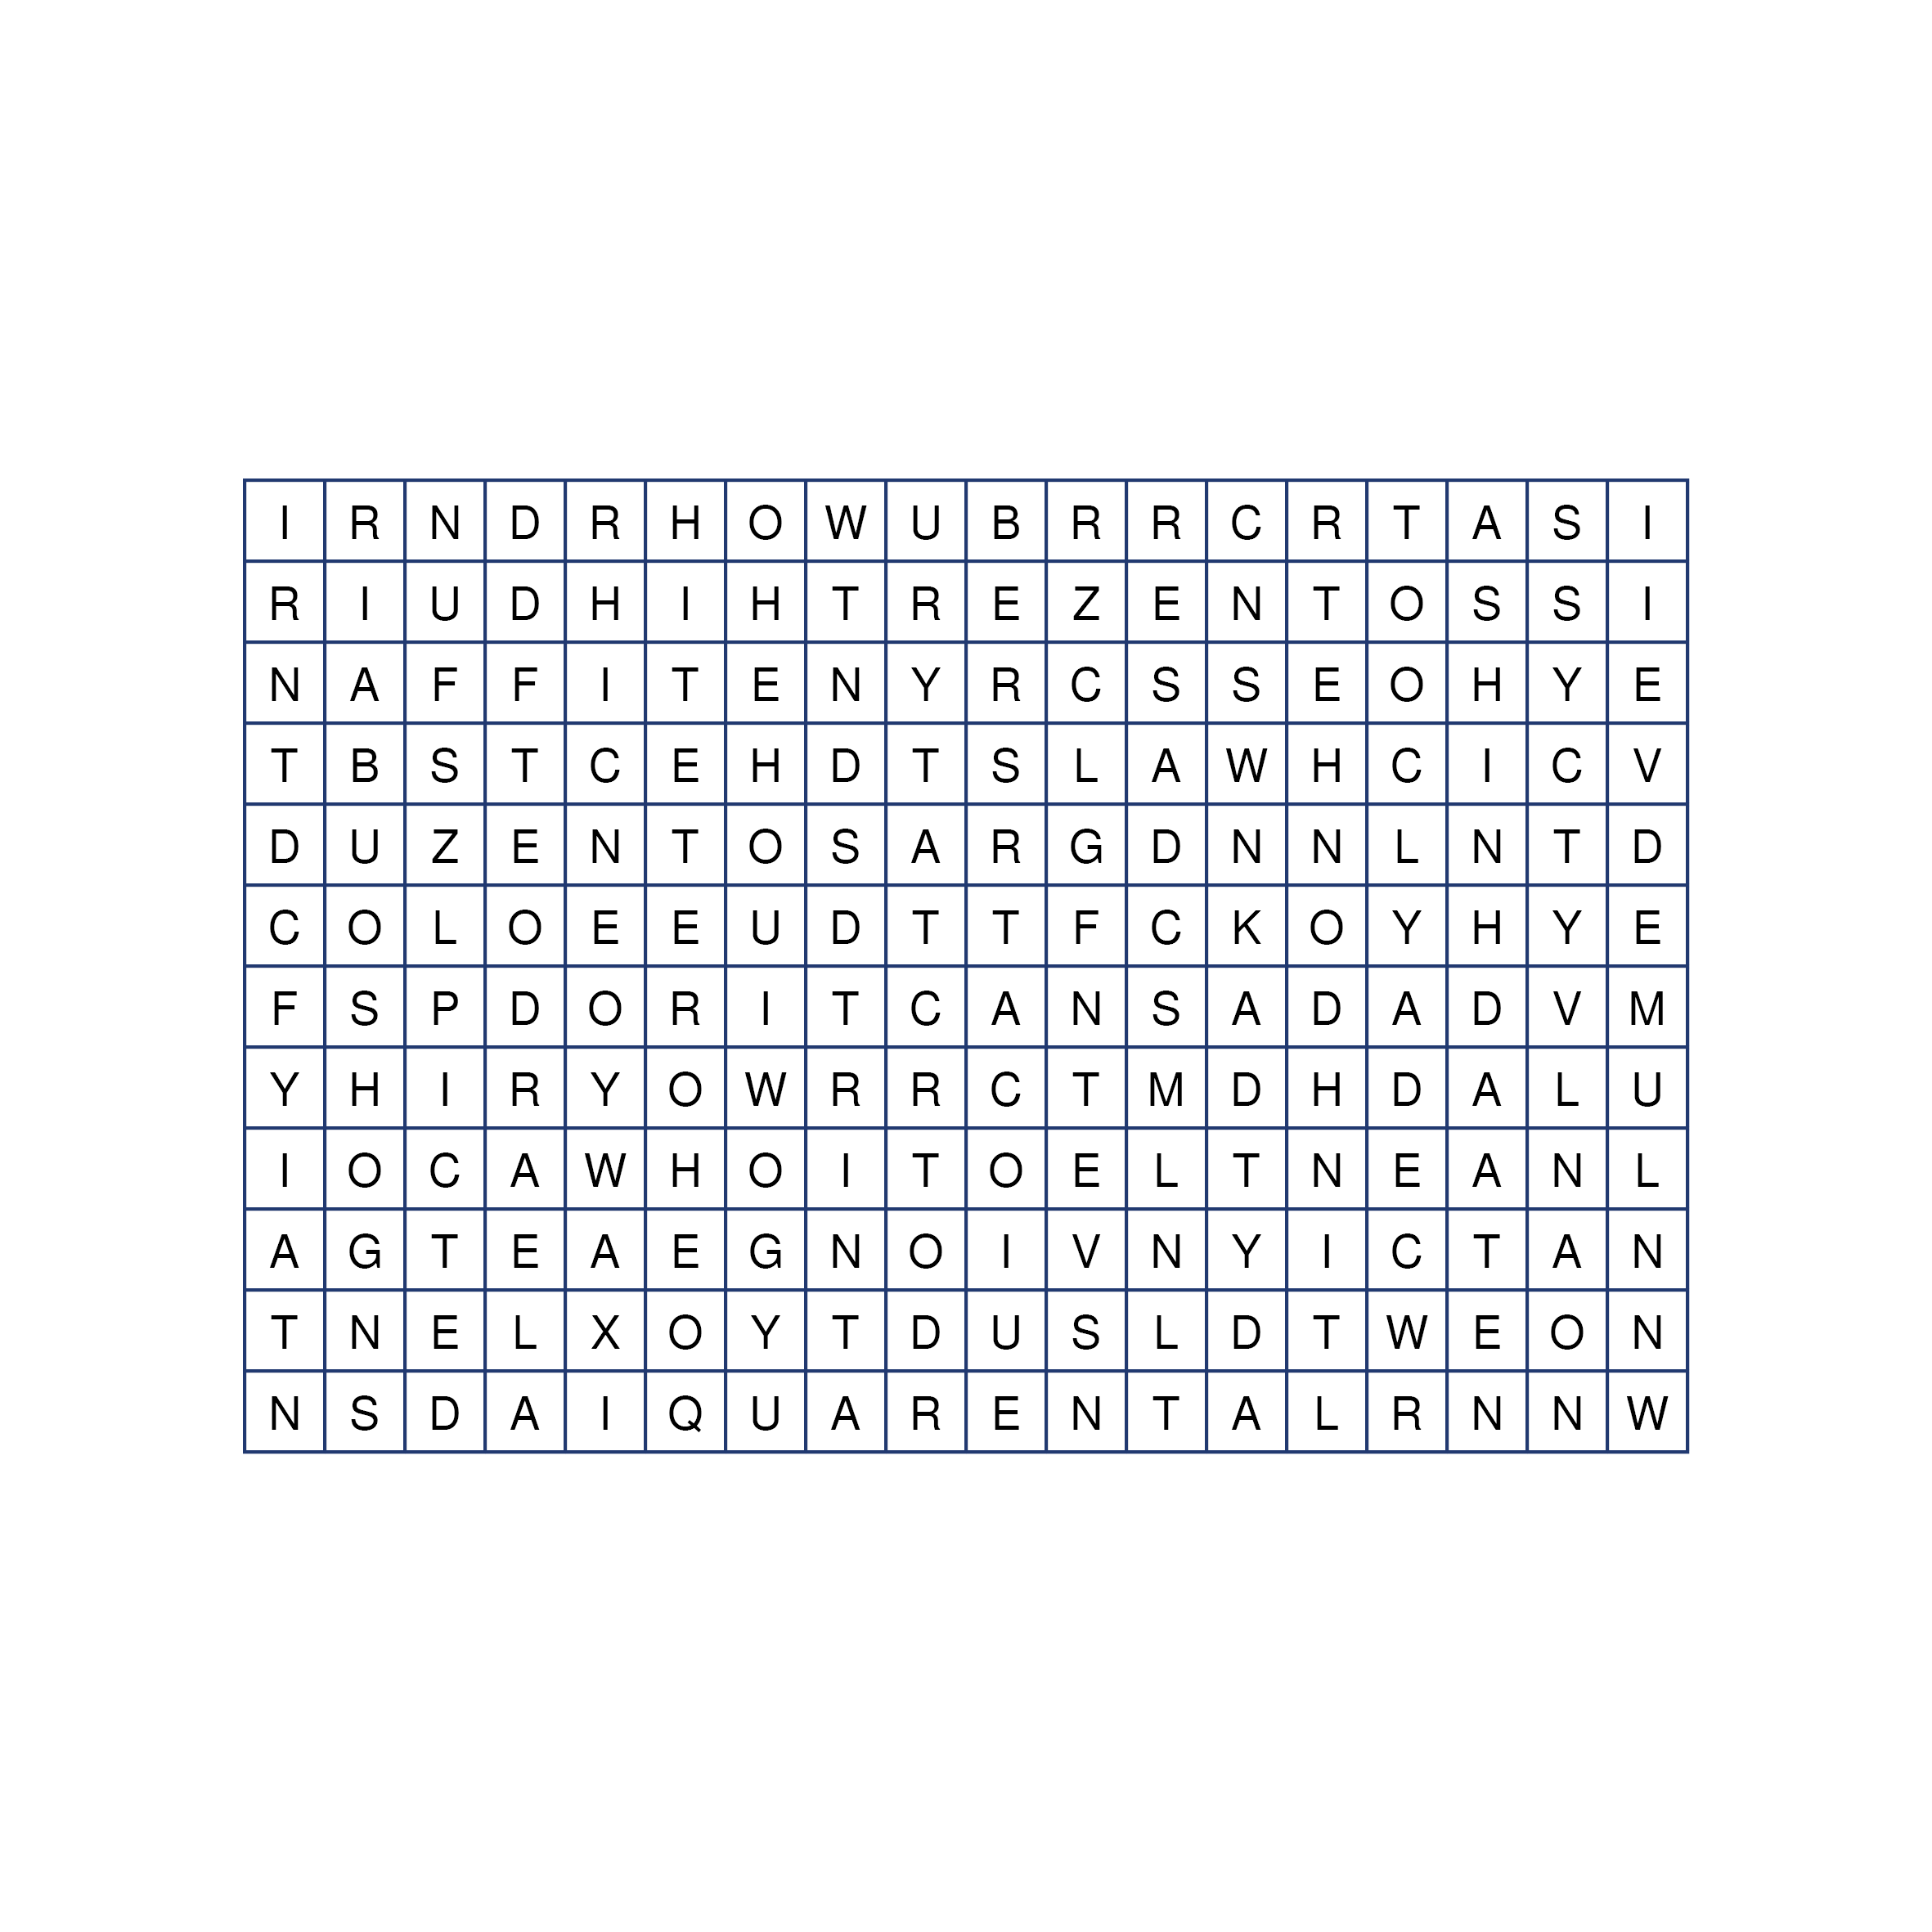
\includegraphics[width=6.27083in,height=3.72904in]{media/image27.png}

Uma medida direta que pode ser tomada pelo governo para melhorar o
acesso à moradia é:

\begin{escolha}
\item a construção de habitações populares.

\item a igualdade salarial entre homens e mulheres.

\item o aumento da segurança em locais públicos.

\item a distribuição de alimentos nas comunidades.
\end{escolha}

\coment{Habilidade BNCC EF05HI04: Associar a noção de cidadania com os
princípios de respeito à diversidade, à pluralidade e aos direitos
humanos.

Habilidade SAEB: 5C2. Avaliar a atuação de diferentes grupos sociais e
seus papéis na organização das cidades e comunidades.

a) Correta. A construção de habitações populares é eficaz para melhorar
o acesso à moradia de pessoas em situação de pobreza;
b) Incorreta. Essa medida não atua diretamente sobre o acesso à moradia;
c) Incorreta. Essa medida garante a segurança, não o acesso à moradia;
d) Incorreta. Essa medida garante a segurança alimentar, e não o acesso
à moradia.}

\chapter{6. Relações de trabalho, produção e circulação}

\coment{Habilidade da BNCC envolvidas:

EF05GE05: Identificar e comparar as mudanças dos tipos de trabalho e
desenvolvimento tecnológico na agropecuária, na indústria, no comércio e
nos serviços.}

%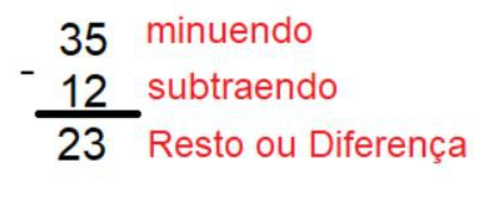
\includegraphics[width=3.13954in,height=2.08333in]{media/image28.png}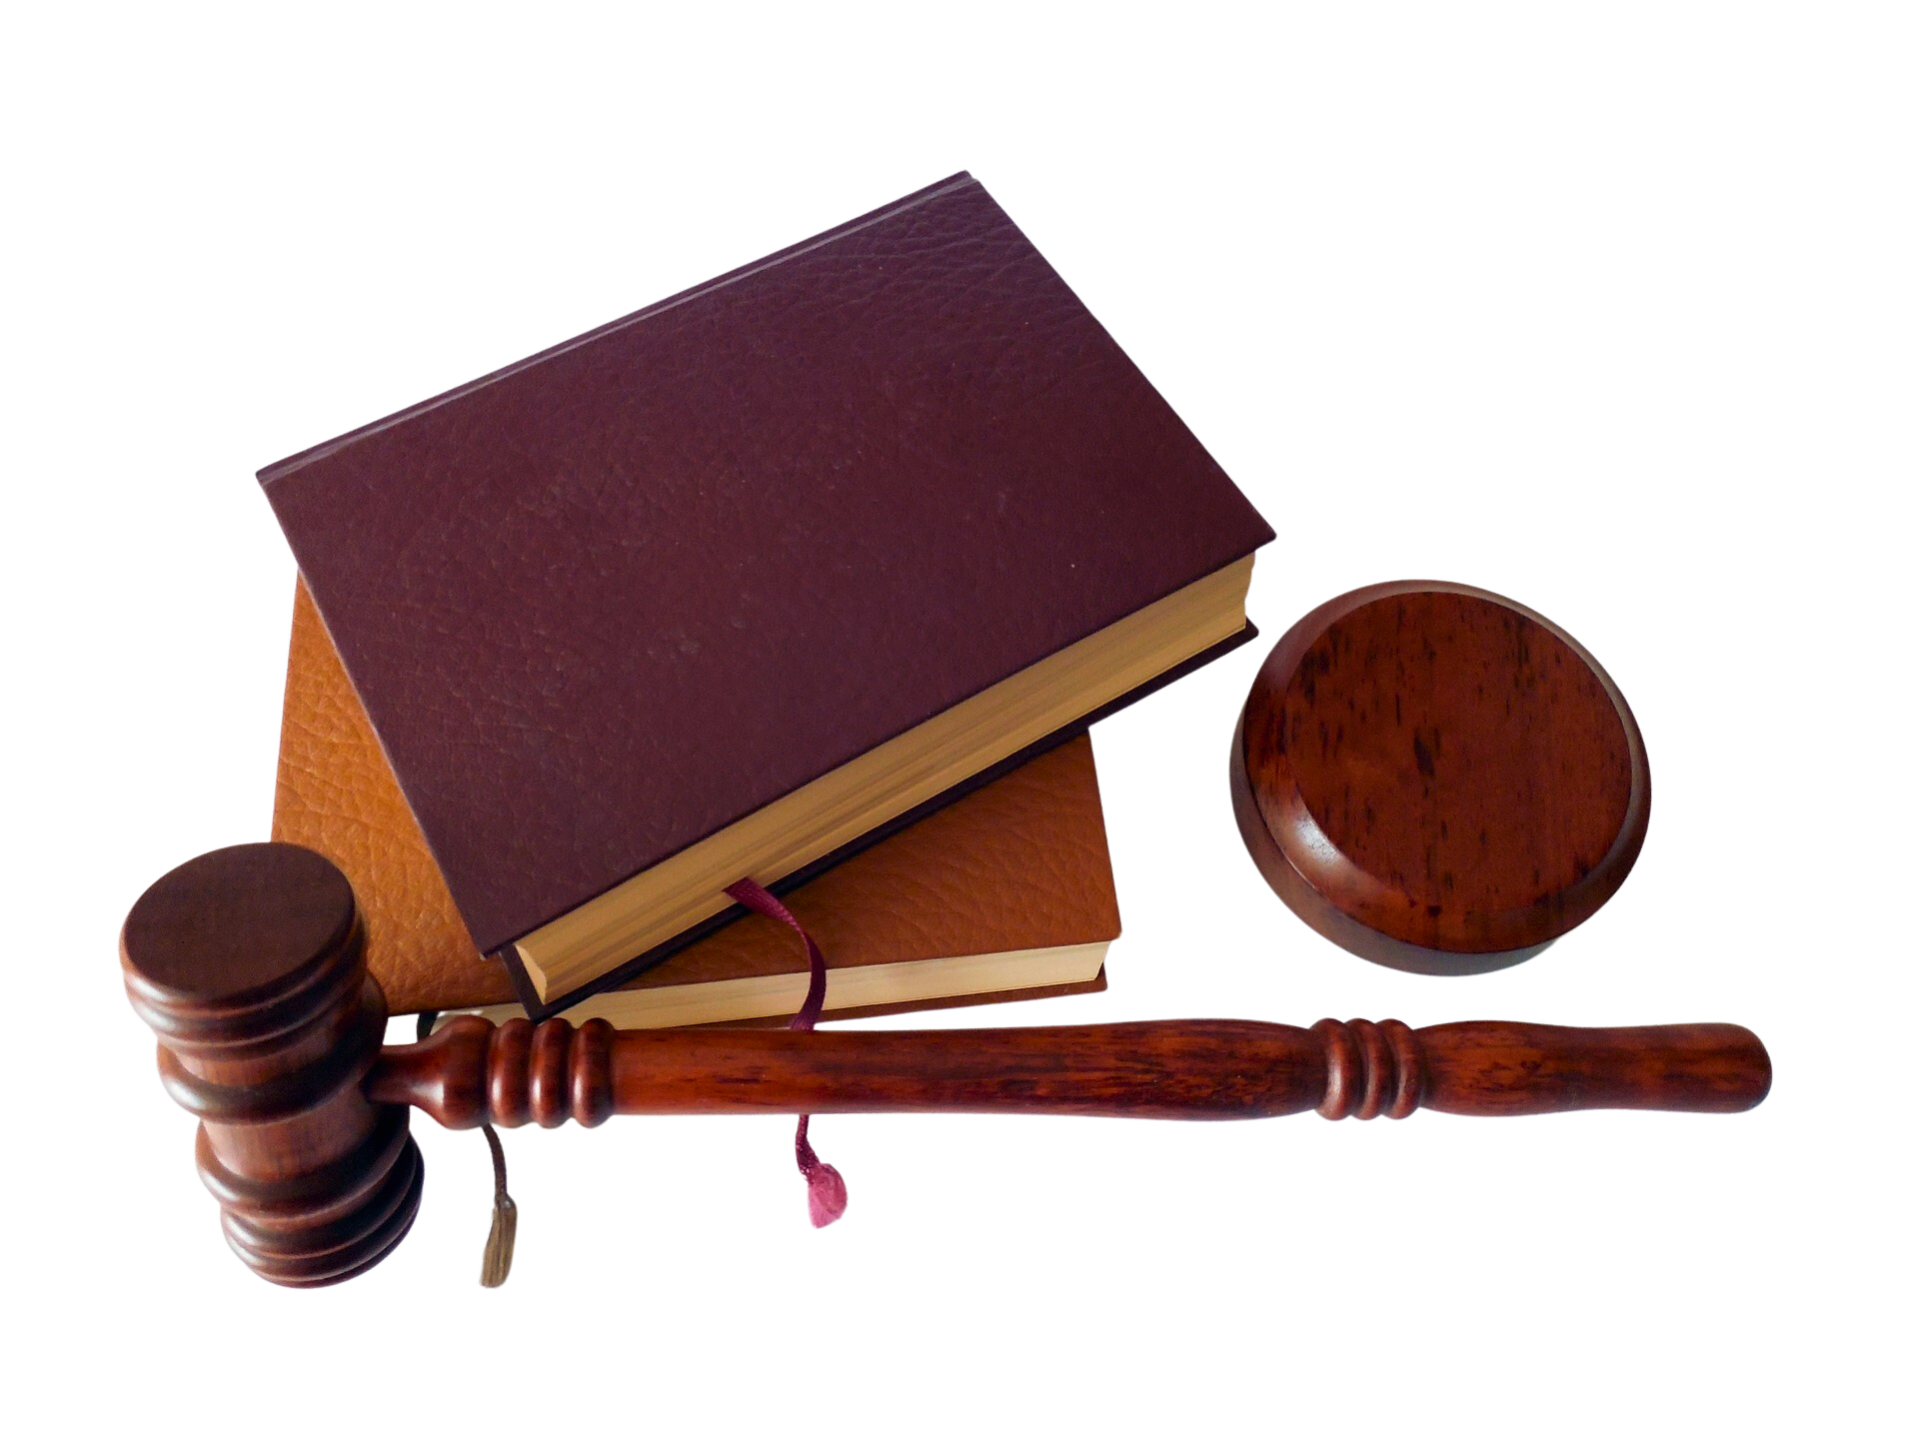
\includegraphics[width=3.20313in,height=2.13542in]{media/image29.png}
%\fonte{Disponível em: \emph{https://br.freepik.com/fotos-gratis/um-agricultor-que-esta-usando-uma-pa-para-cavar-o-solo-em-seus-campos-de-arroz\_5491642.htm\#query=trabalho\%20terra\&position=16\&from\_view=search\&track=ais} Acesso em: 23 fev. 2023.}
%\fonte{Disponível em: \emph{https://br.freepik.com/fotos-gratis/mulher-de-close-up-costurando-com-maquina\_12810036.htm\#query=trabalho\%20costura\&position=18\&from\_view=search\&track=ais} Acesso em: 23 fev. 2023.}

\conteudo{Vocês conhecem os diferentes tipos de trabalho que existem no Brasil e
no mundo? E como eles impactam em como nós vivemos, no que comemos, no
que fazemos? Tudo o que temos e consumimos no nosso dia a dia vem do
trabalho de alguém. O arroz e feijão que comemos todos os dias foi
plantado e colhido por um trabalhador do campo, transportado por um
outro trabalhador, separado e vendido no mercado onde trabalham muitas
outras pessoas. A roupa que utilizamos também foi costurada por um
trabalhador. Em seguida, foi levada a um centro comercial, onde nossos
pais compraram com a ajuda de um vendedor.

Muitas vezes não temos ideia de que objeto tão simples que utilizamos em
nosso cotidiano chegou até nós através de uma rede muito grande de
pessoas depois de ter produzido, transportado, embalado, e vendido por
dezenas de trabalhadores.

Neste módulo vamos estudar esses diversos tipos de trabalho, e entender
como eles são importantes para o nosso dia a dia.}

\colorsec{Atividade 1}

\coment{EF05GE05: Identificar e comparar as mudanças dos tipos de trabalho e
desenvolvimento tecnológico na agropecuária, na indústria, no comércio e
nos serviços.

SAEB: 7A4: Reconhecer características das atividades minerais,
agropecuárias e industriais.

7A8: Identificar diferentes formas de trabalho realizadas no campo.}

Observem as imagens

%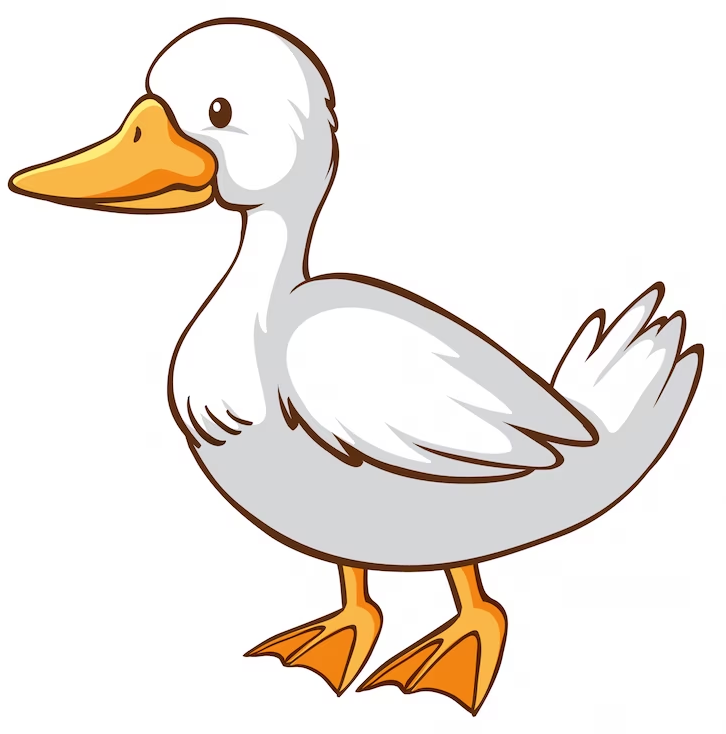
\includegraphics[width=3.26563in,height=2.17708in]{media/image30.png}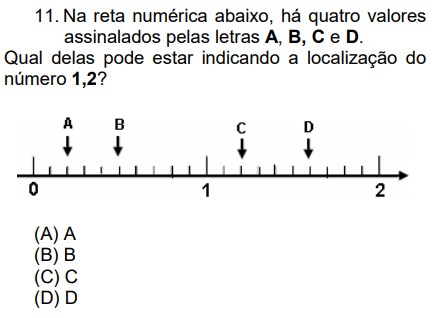
\includegraphics[width=3.26563in,height=2.17708in]{media/image31.png}
%\fonte{Disponível em: \emph{https://br.freepik.com/fotos-gratis/cavaleiro-liderando-um-rebanho-de-animais-em-uma-fazenda-na-australia\_9990935.htm\#query=pecu\%C3\%A1ria\&position=12\&from\_view=search\&track=sph} Acesso em 22 fev. 2023.}

%\fonte{Disponível em: \emph{https://br.freepik.com/fotos-gratis/tantos-vegetais-neste-campo\_10729697.htm\#query=agricultura\&position=8\&from\_view=search\&track=sph} Acesso em: 22 fev. 2023}

\num{a} Você reconhece algum desses lugares? Você já visitou ou viu com seus
próprios olhos algo parecido?

\linhas{2}

\coment{Espera-se que o aluno tente reconhecer, em sua cidade ou bairro, uma
paisagem parecida a esta para, assim, entender o que se passa com os
trabalhadores que atuam naquele local e o que eles representam para sua
comunidade.}

\num{b} Com a ajuda de seu professor, preencha a tabela com características
sobre cada uma das imagens:

\begin{tabular}{l|l}
\hline
\textbf{Imagem 1} & \textbf{Imagem 2} \\ \hline
\begin{tabular}[c]{@{}l@{}}Nome da atividade:\\ \rosa{Pecuária}\end{tabular} & \begin{tabular}[c]{@{}l@{}}Nome da atividade:\\ \rosa{Agricultura}\end{tabular} \\ \hline
Local: \rosa{Campo} & Local: \rosa{Campo} \\ \hline
\begin{tabular}[c]{@{}l@{}}Principal produto do trabalho:\\ \rosa{Alimentos de origem animal}\end{tabular} & \begin{tabular}[c]{@{}l@{}}Principal produto do trabalho:\\ \rosa{Alimentos de origem vegetal}\end{tabular} \\ \hline
\end{tabular}

\num{c} Agora, associe com uma seta os tipos de produto com o trabalho presente em cada uma das imagens:

\begin{multicols}{2}

Imagem 1

Imagem 2

\columnbreak

Leite

Arroz

Carne bovina

Alface
\end{multicols}

\coment{Resposta: Leite e carne bovina devem estar ligados com a Imagem 1 e
Arroz e Alface com a Imagem 2}

\colorsec{Atividade 2}

Agora, vamos falar sobre Agricultura

\coment{EF05GE05: Identificar e comparar as mudanças dos tipos de trabalho e
desenvolvimento tecnológico na agropecuária, na indústria, no comércio e
nos serviços.

Habilidade SAEB: 7A11: Reconhecer usos de tecnologia no contexto do
campo e da agropecuária.

7B8: Compreender as transformações nas relações entre campo e cidade
envolvendo os fluxos de trabalhadores.

7A2: Reconhecer os fluxos de migração entre a cidade e o campo.}

Vamos observar essas duas imagens:

%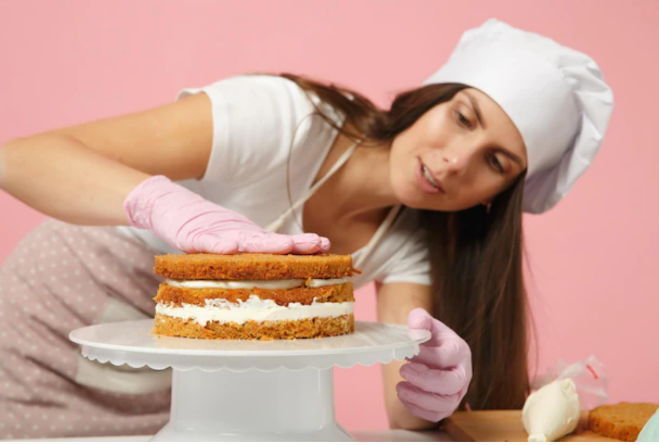
\includegraphics[width=3.05208in,height=2.03114in]{media/image32.png}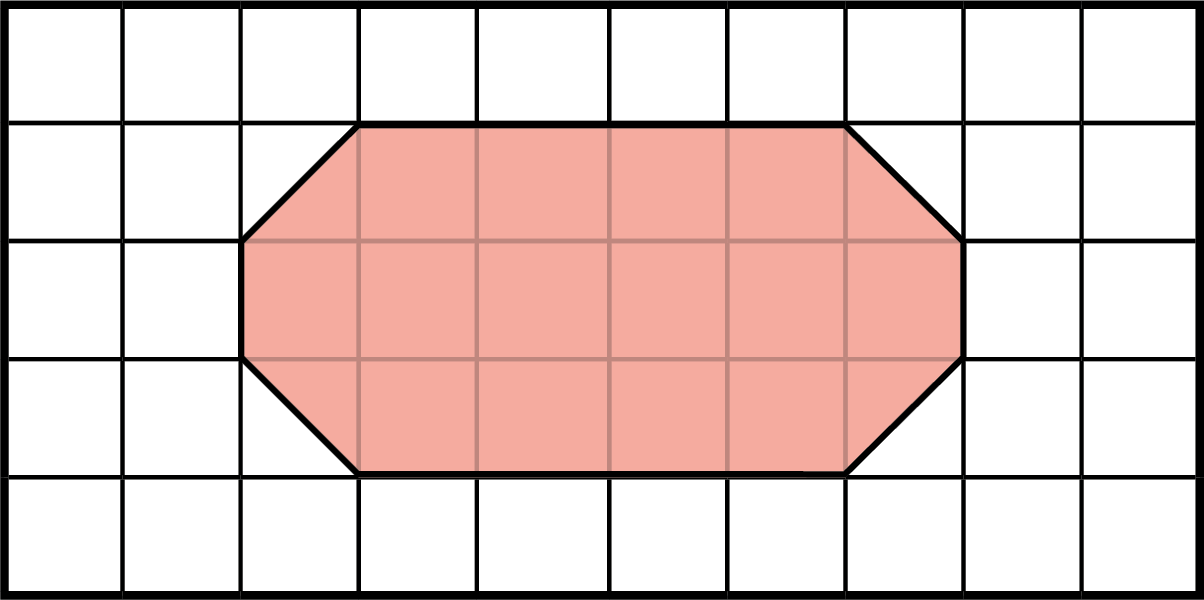
\includegraphics[width=3.05723in,height=2.03646in]{media/image33.png}
%Imagem 1. Disponível em: \emph{https://br.freepik.com/fotos-gratis/agricultura-e-conceito-de-producao-de-alimentos-com-silos-de-maquina-de-trator-e-sistema-de-irrigacao\_11133942.htm\#query=agricultura\&position=24\&from\_view=search\&track=sph} Acesso em: 22 fev. 2023.

%Imagem 2. Disponível em: \emph{https://br.freepik.com/fotos-gratis/retrato-de-agricultor-agronomo-senior-trabalhador-em-um-campo-de-milho-verificando-as-colheitas-antes-da-colheita\_11450848.htm\#query=agricultura\&position=35\&from\_view=search\&track=sph} Acesso em: 22 fev. 2023.

\num{a} O que você observa de igual entre elas?

\linhas{2}
\coment{Ambas retratam cenas da produção agrícola.}

\num{b} E de diferente?

\linhas{2}
\coment{Em uma, o trator faz o trabalho, na outra, o trabalhador atua
diretamente com a colheita.}

\num{c} O que você acha que muda de uma forma de agricultura para a outra de
maneira positiva? Anote as informações passadas pela professora. 

\linhas{3}

\coment{Aqui, fale sobre a influência que as novas tecnologias tiveram para o
desenvolvimento da agricultura. Fale sobre a maior produtividade e
oferta de alimentos à população.}

\num{d} Você acha que o uso de novas tecnologias na agricultura pode ser ruim de
algum jeito? No que ele impacta na vida dos trabalhadores?

\linhas{3}
\coment{Fale sobre a diminuição da oferta de emprego nos campos uma vez que as
máquinas tomam o lugar dos trabalhadores. Fale sobre os movimentos de
migração do campo em busca de empregos na cidade.}

Vamos ver alguns dados sobre esse processo:

\begin{quote}
Com a ``modernização conservadora'' ocorreu uma diminuição significativa
da oferta de trabalho no campo na região Centro-Oeste e principalmente
no Estado de Goiás. De acordo com o IBGE -- Instituto Brasileiro de
Geografia e Estatística - entre 1985 e 1996 houve uma redução de 20\%
dos trabalhadores rurais no Centro-Oeste.

Em 1985, existiam cerca 1,5 milhão de trabalhadores no campo, e em 1996,
os trabalhadores rurais somavam aproximadamente 1,2 milhão de
trabalhadores. Em Goiás, em 1985, os trabalhadores rurais somavam
616.000.

Uma década depois (1996) existiam cerca de 472.000 trabalhadores rurais,
ocorrendo uma redução de aproximadamente 23\%, expressando as mudanças
no trabalho após a adoção das inovações técnicas.

Mendonça, M. R. (2011). A Modernização da Agricultura e os impactos
sobre o trabalho. \textbf{PEGADA - A Revista Da Geografia Do Trabalho,
3}. https://doi.org/10.33026/peg.v3i0.789
\end{quote}

\colorsec{Atividade 3}

Agora, vamos ver como esse processo dá origem a outro: \textbf{a migração}.

\coment{BNCC EF05GE05: Identificar e comparar as mudanças dos tipos de trabalho
e desenvolvimento tecnológico na agropecuária, na indústria, no comércio
e nos serviços.

SAEB 7C1: Avaliar o papel desempenhado pela migração e seus efeitos nas
regiões de destino.

7B8: 8. Compreender as transformações nas relações entre campo e cidade
envolvendo os fluxos de trabalhadores.

7B2: Analisar diferentes fluxos populacionais e suas contribuições para
a formação da sociedade brasileira.}

Segundo Mendonça, a modernização no campo "historicamente promoveu a
migração forçada dos trabalhadores (pequenos produtores rurais)
resultando em expropriação fundiária que `esvazia o campo e urbaniza a
sociedade'." Ou seja, a falta de empregos no campo levou os
trabalhadores a irem para a cidade em busca de novas oportunidades de
trabalho.

\fonte{Mendonça, M. R. (2011). A Modernização da Agricultura e os impactos
sobre o trabalho. \textbf{PEGADA - A Revista Da Geografia Do Trabalho,
3}. \emph{https://doi.org/10.33026/peg.v3i0.789}}

\num{a} Você sabe o que é migração? Descreva abaixo com a ajuda de sua
professora.

\linhas{3}
\coment{Definir migração para o aluno: movimentação de entrada (imigração) ou
saída (emigração) de indivíduo ou grupo de indivíduos, em busca de
melhores condições de vida {[}Essa movimentação pode ser entre países
diferentes ou dentro de um mesmo país.{]}.

\fonte{Fonte:
\emph{https://languages.oup.com/google-dictionary-pt/}}
}

\num{b} Você conhece alguém que já migrou? Qual foi o motivo? Converse com seus
colegas sobre isso.

\coment{Aqui o aluno deve relembrar suas próprias experiências. É comum que
alguém da família tenha vindo de algum lugar, mudado de cidade ou estado
por motivos familiares, financeiros, entre outros. Deixe que os alunos
conversem e compartilhem suas experiências.}

\num{c} Observe a imagem e responda:

%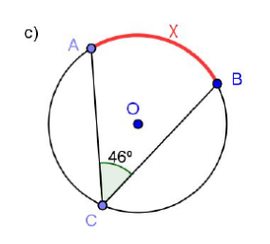
\includegraphics[width=4.54284in,height=3.02604in]{media/image34.png}
%Disponível em: \emph{https://br.freepik.com/fotos-gratis/steel-business-predio-urbano-observacao\_1046153.htm\#query=S\%C3\%A3o\%20Paulo\&position=2\&from\_view=search\&track=ais} Acesso em: 23 fev. 2023.

O que você acha que pode acontecer se muitas pessoas migram para um mesmo lugar rapidamente, por exemplo, em uma cidade?

\linhas{3}
\coment{Fale com os alunos sobre as consequências de uma migração forçada, no
caso dos trabalhadores rurais que perderam seus empregos por causa da
tecnologia. Fale sobre como o crescimento desordenado das cidades pode
afetar na vida das pessoas que moram lá, e pode trazer graves
consequências de precarização na saúde, moradia, e no trabalho.}

\colorsec{Atividade 4}

\coment{BNCC EF05GE05: Identificar e comparar as mudanças dos tipos de trabalho
e desenvolvimento tecnológico na agropecuária, na indústria, no comércio
e nos serviços.

SAEB 7C5: Avaliar a importância dos caminhos terrestres, fluviais ou
marítimos para a dinâmica da vida comercial.

7C9. Avaliar a importância das diversas formas de trabalho existentes,
propondo estratégias para sua valorização.}

Observe as imagens.

%
\includegraphics[width=3.08068in,height=2.05208in]{media/image35.png}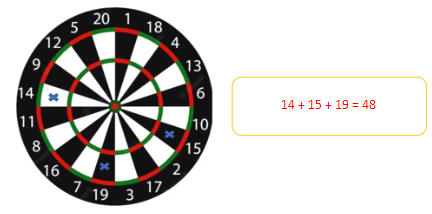
\includegraphics[width=3.07665in,height=2.04940in]{media/image36.png}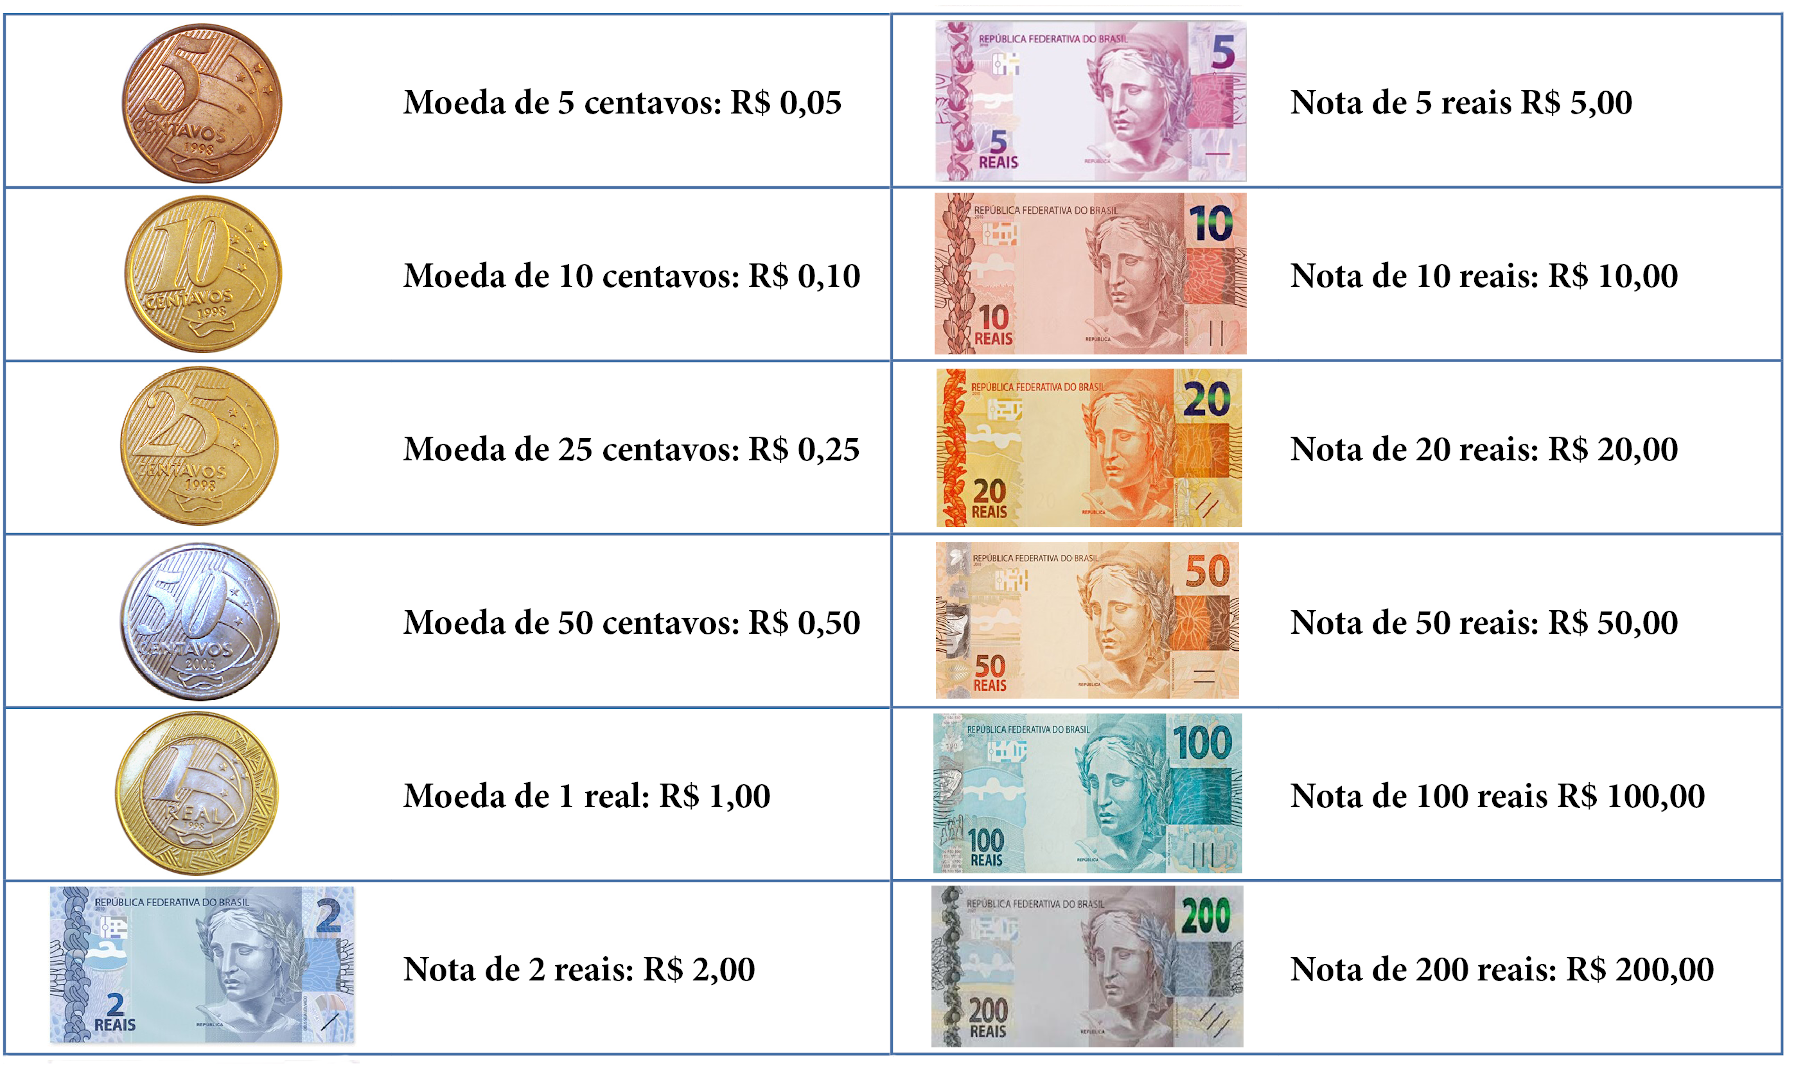
\includegraphics[width=3.07292in,height=2.04493in]{media/image37.png}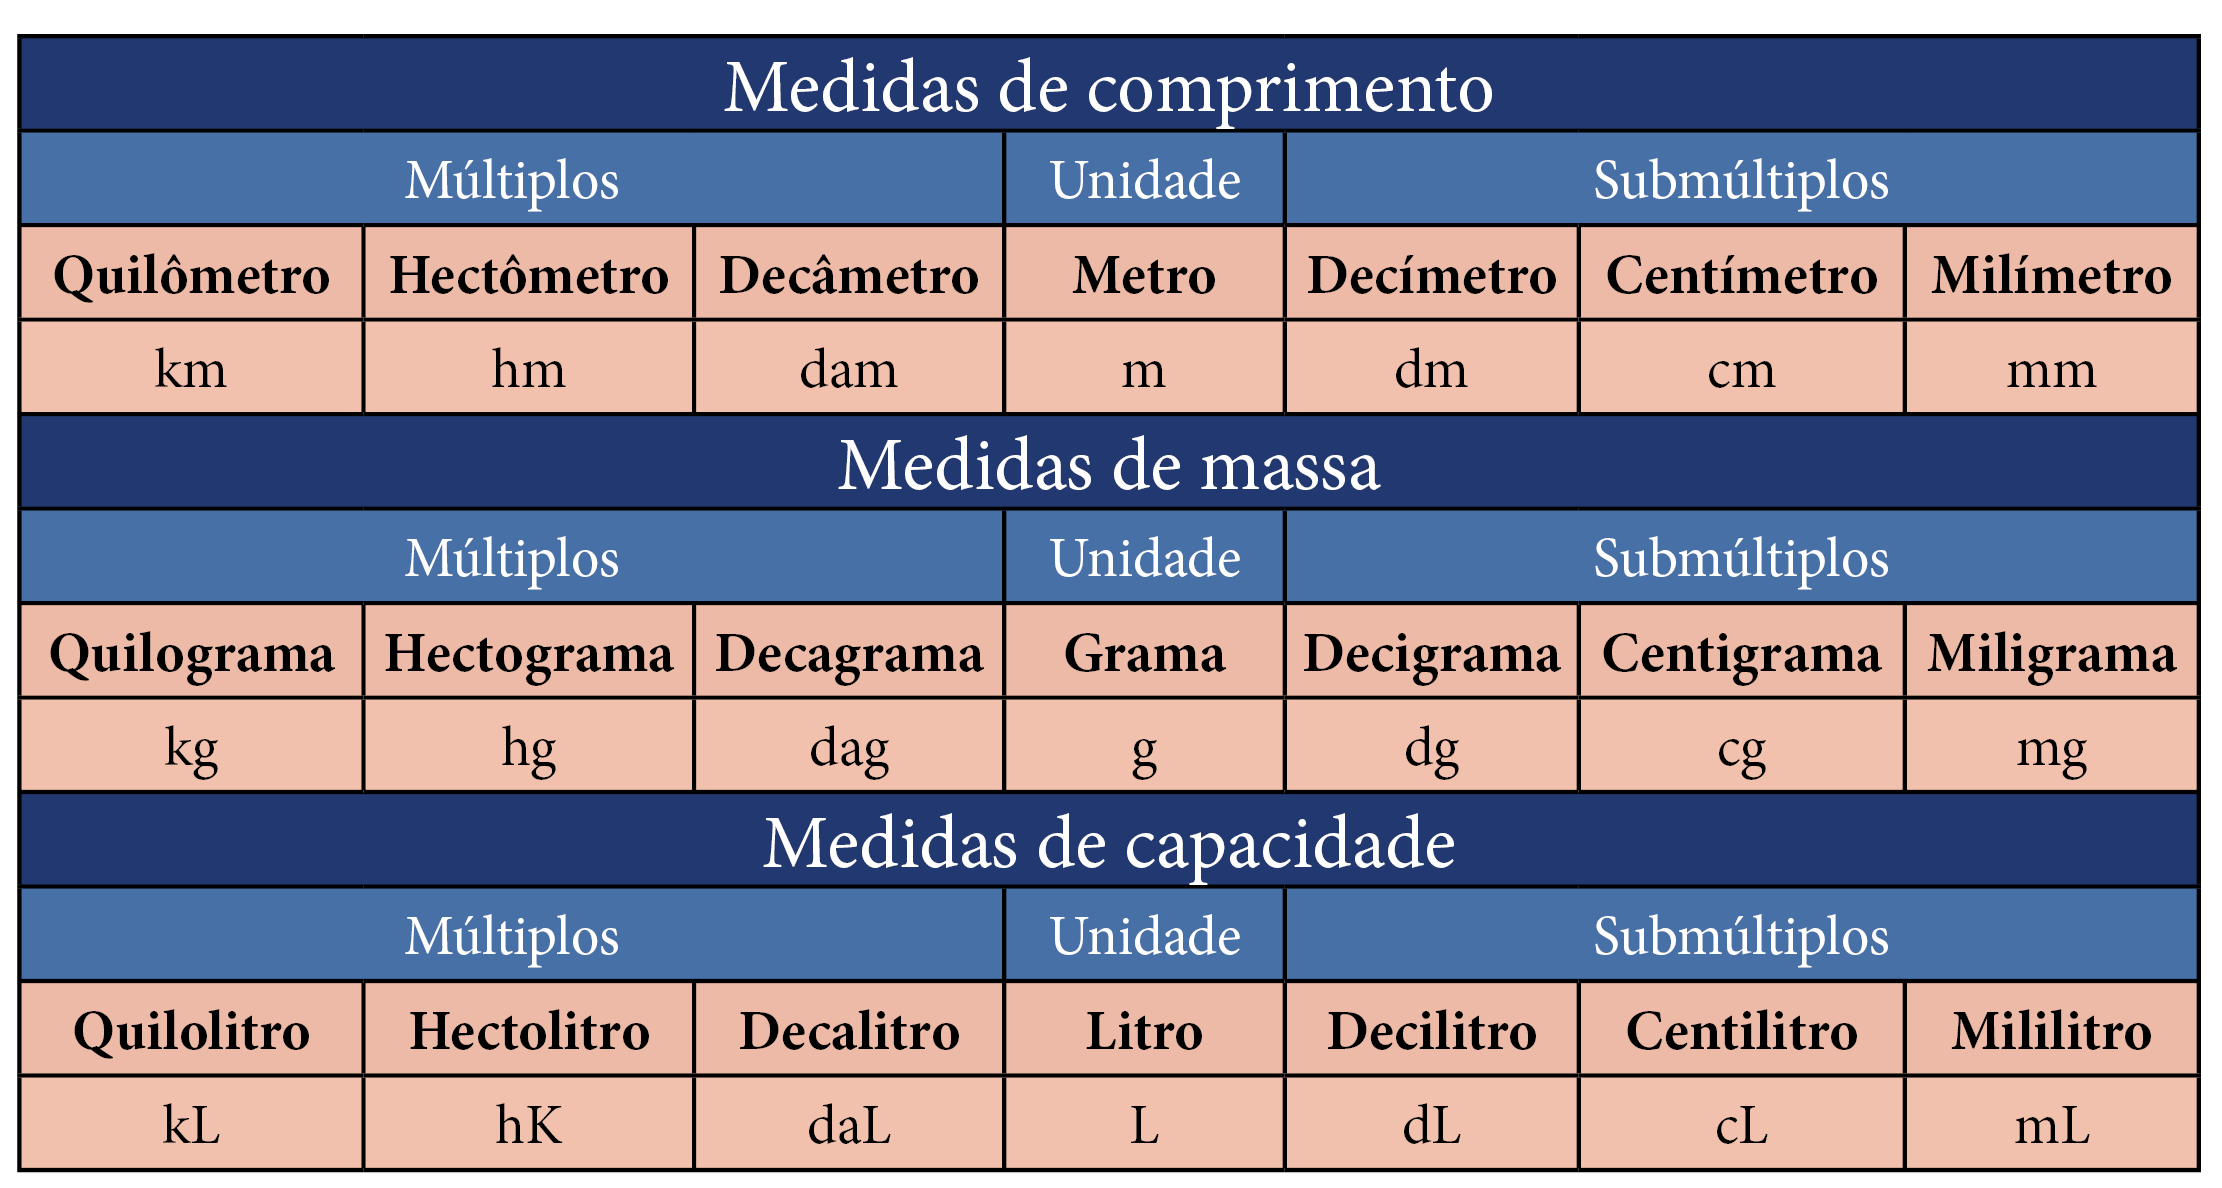
\includegraphics[width=3.07292in,height=2.05308in]{media/image38.png}

%1)Caminhão: \emph{https://br.freepik.com/fotos-gratis/caminhoes-de-reboque-dirigindo-na-estrada-cercados-por-belas-arvores-verdes\_9932046.htm\#query=caminh\%C3\%A3o\&position=6\&from\_view=search\&track=sph}

%2)Barco: \emph{https://br.freepik.com/fotos-gratis/vista-aerea-do-navio-de-carga-do-conteiner-no-mar\_13180387.htm\#query=barco\%20carga\&position=0\&from\_view=search\&track=ais}

%3)Trem: \emph{https://br.freepik.com/fotos-gratis/vagoes-de-trem-transportando-conteineres-de-carga-para-empresas-de-navegacao\_11136398.htm\#query=ferrovia\&position=1\&from\_view=search\&track=sph}

%4)Avião: \emph{https://br.freepik.com/fotos-gratis/aviao-ao-por-do-sol\_4291511.htm\#query=avi\%C3\%A3o\&position=11\&from\_view=search\&track=sph}

\num{a} As quatro imagens representam quatro vias de transportes que utilizamos
para a \textbf{circulação de mercadorias} no Brasil. Você sabe o nome
delas? Com a ajuda de sua professora, complete na ordem das imagens:
Colocar quatro linhas numeradas.

\begin{enumerate}
\item \preencher \coment{Rodovia (estradas)}

\item \preencher \coment{Hidrovia (rios e mares)}

\item \preencher \coment{Ferrovia (Trens e locomotivas)}

\item \preencher \coment{Aerovia (Aviões)}

\end{enumerate}

Ainda, são pessoas que comandam cada um desses transportes. Vamos ler um
pouco sobre o trabalho de um caminhoneiro nesta reportagem sobre o Dia
do Caminhoneiro:

\begin{quote}
\textbf{Dia do Caminhoneiro: motoristas falam sobre os desafios de
exercer a profissão}

São horas atrás do volante, dias fora de casa e metas a cumprir. Saudade
da família e os perigos nas estradas fazem parte da rotina diária dos
motoristas de cargas.

Casado, pai de um menino de 15 anos e de uma menina de 1 ano e 6 meses,
Costa disse que conversa com a família todos os dias. "Quando eu comecei
a trabalhar, meu menino já era grandinho e às vezes ele ia comigo nas
viagens mais curtas. Agora com a pequenininha ficou mais dolorido ficar
fora de casa'', afirmou ele.

``Para você estar usando seu celular hoje, chegou até você por um
caminhão. Seu carro não anda se você não tiver combustível, que chega
até o posto por meio de um caminhão. O café da manhã, aquele leite,
aquela farinha que fez o pão, tudo passou por um caminhão'', disse.

\fonte{Disponível em:
\emph{https://g1.globo.com/sp/sao-carlos-regiao/noticia/dia-do-caminhoneiro-motoristas-falam-sobre-os-desafios-de-exercer-a-profissao.ghtml}
Acesso em: 23 fev. 2023.}
\end{quote}

\num{b} Segundo o texto, qual é a importância do trabalho de pessoas como Costa?

\linhas{2}
\coment{A partir de seu trabalho chega até nós tudo que temos acesso em nosso
dia a dia, como comida, roupas, objetos da casa, etc.}

\num{c} Com a ajuda de seus colegas, faça uma lista de outras profissões que
você acha que também são importantes no processo de circulação de
mercadorias até chegar em nossa casa:

\begin{enumerate}
\item \preencher

\item \preencher

\item \preencher

\item \preencher

\item \preencher

\item \preencher

\item \preencher

\item \preencher
\end{enumerate}

\coment{Nesse momento, deixe que os alunos conversem entre si para chegar nas
profissões. Você pode anotar na lousa as profissões que forem surgindo
ao longo do debate.}

\colorsec{Treino}

\num{1}

%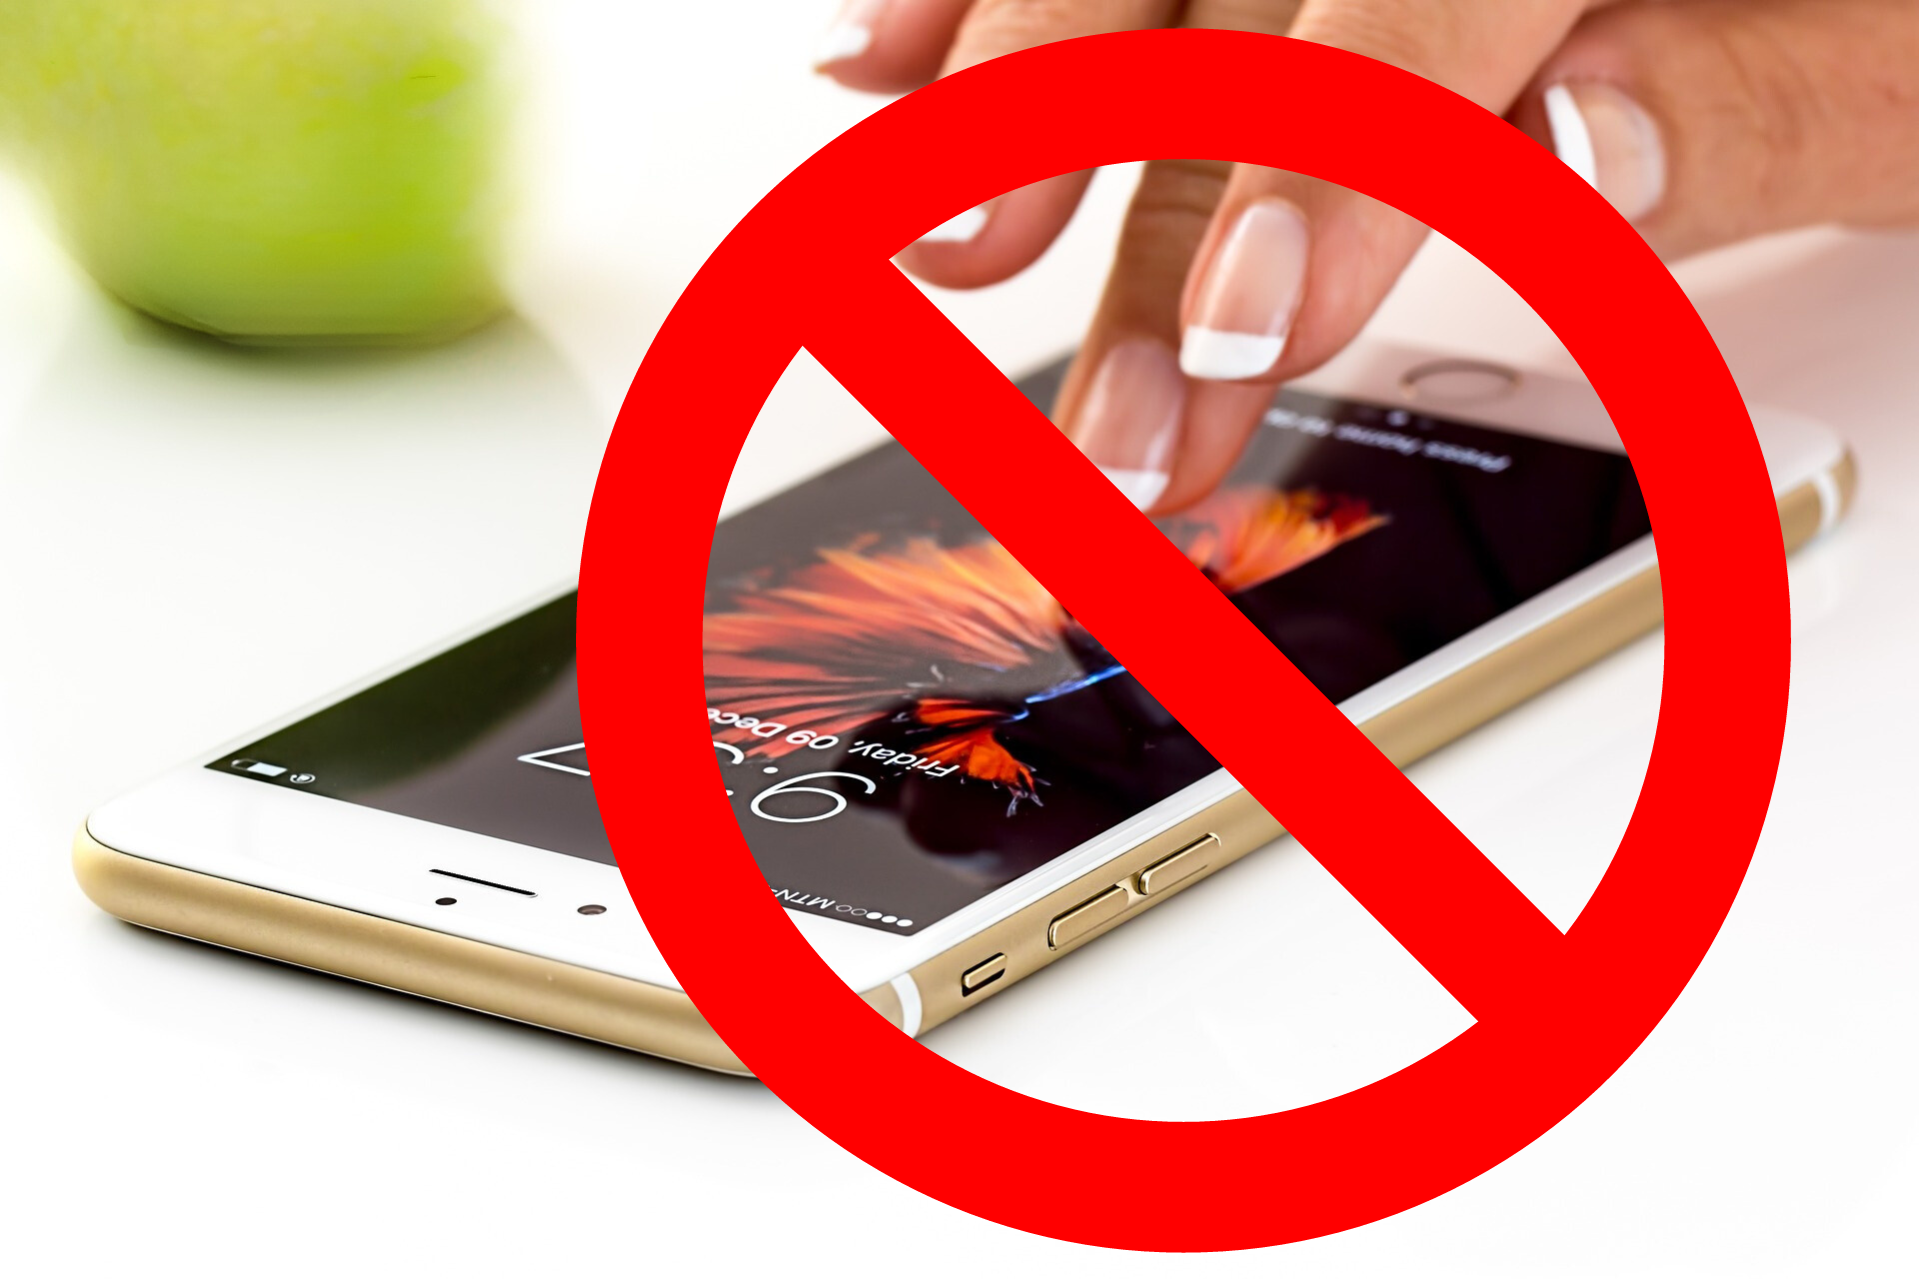
\includegraphics[width=4.92188in,height=3.27852in]{media/image39.png}
%Disponível em: \emph{https://br.freepik.com/fotos-gratis/interior-de-oficina-de-fabrica-e-maquinas-em-fundo-de-producao-de-vidro\_26150555.htm\#query=ind\%C3\%BAstria\&position=26\&from\_view=search\&track=sph} Acesso em: 23 fev. 2023

A imagem acima representa a seguinte forma de trabalho:

\begin{escolha}
\item Pecuária.

\item Agrícola.

\item Industrial.

\item Mineral.
\end{escolha}

\coment{BNCC EF05GE05: Identificar e comparar as mudanças dos tipos de trabalho
e desenvolvimento tecnológico na agropecuária, na indústria, no comércio
e nos serviços.

SAEB: 7A4. Reconhecer características das atividades minerais,
agropecuárias e industriais.

a) Incorreto. Não se trata de um pasto, mas de uma indústria;
b) Incorreto. Não se trata de uma plantação, mas de uma indústria;
c) Correto. Se trata de uma indústria;
d) Incorreto. Não se trata de uma mina, mas de uma indústria.}

\num{2} As metrópoles do século 21 mesclam trens, automóveis, ônibus e bondes
com o resgate de opções antigas e mais sustentáveis, como a bicicleta.
Contudo, ao longo da história, pessoas e cargas já foram movimentadas
por veículos bem diferentes dos que conhecemos hoje: meios de transporte
antigos que não são mais usados em larga escala acabaram virando peça de
museu ou objeto de curiosidade.

\fonte{Disponível em:
\emph{https://summitmobilidade.estadao.com.br/ir-e-vir-no-mundo/meios-de-transporte-antigos-4-modais-que-nao-existem-mais/}
Acesso em: 23 fev. 2022}

Um exemplo de transporte antigo usado para o deslocamento de mercadorias é

\begin{escolha}
\item avião de carga.

\item carruagem à cavalo.

\item caminhão carreta.

\item motos de delivery.
\end{escolha}

\coment{BNCC EF05GE05: Identificar e comparar as mudanças dos tipos de trabalho
e desenvolvimento tecnológico na agropecuária, na indústria, no comércio
e nos serviços.

SAEB: 7B19. Relacionar os diferentes meios de transporte ou comunicação
aos seus tempos históricos.

7B3: Analisar as transformações ocorridas nos processos de deslocamento
das pessoas ou mercadorias.

7A14: Reconhecer os diferentes modais de transporte e suas
características.

a) Incorreta. O avião é um transporte atual e não antigo;
b) Correta. A carruagem à cavalo era utilizada antigamente para o
transporte de mercadorias;
c) Incorreta. O caminhão carreta é um transporte moderno;
d) Incorreta. As motos são veículos modernos, e não são consideradas
veículos de carga.}

\num{3} A história da descoberta do vidro é bem antiga, e os primeiros
registros datam de 5000 a.C. Em 1952, foi revelada uma invenção que
mudou tudo. Fazendo flutuar vidro derretido em estanho também derretido,
Pilkington conseguiu produzir vidro quase tão plano quanto suas placas
prensadas e polidas, a uma espessura econômica e em grandes quantidades,
através de um processo contínuo. Essa única invenção revolucionou e
petrificou a indústria.

%\fonte{Disponível em: \emph{https://vidrado.com/noticias/historia/historia-da-producao-do-vidro/} Acesso em: 23 fev. 2023.}

O texto fala sobre a

\begin{escolha}
\item falta de estudos técnicos sobre materiais descobertos na antiguidade.

\item necessidade de manter técnicas tradicionais na produção em massa.

\item importância de novas tecnologias para o desenvolvimento industrial.

\item dificuldade de viver em sociedades antigas que não tinham indústrias.
\end{escolha}

\coment{BNCC EF05GE05: Identificar e comparar as mudanças dos tipos de trabalho
e desenvolvimento tecnológico na agropecuária, na indústria, no comércio
e nos serviços.

7B11:Compreender o papel e o uso de ferramentas, máquinas e insumos para
a produção de mercadorias.

a) Incorreta. O texto não fala sobre a falta de estudos, mas sim sobre
os avanços nestes;
b) Incorreta. O texto não fala sobre técnicas tradicionais, mas sobre
novas;
c) Incorreta. O texto fala justamente sobre a importância do
desenvolvimento de novas técnicas para o despontamento do vidro;
d) Incorreta. O texto não fala sobre a vida em sociedades antigas nem a
qualifica.}

\chapter{Simulado 1}

\num{1}

%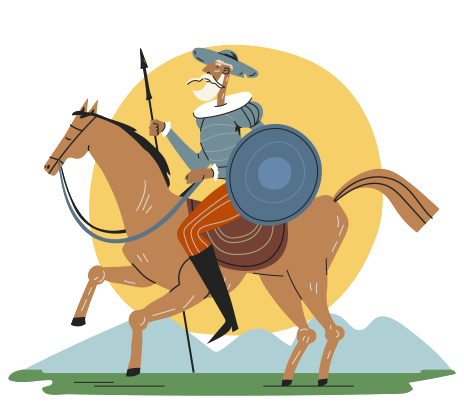
\includegraphics[width=4.26563in,height=3.19568in]{media/image40.png}
%Disponível em: \emph{https://br.freepik.com/fotos-gratis/tempo-sino-acordar-branco-velho\_1044180.htm\#query=rel\%C3\%B3gio\&position=15\&from\_view=search\&track=sph} Acesso em: 23 fev. 2023.

Além do relógio, um outro objeto que nos ajuda a contar o tempo é:

\begin{escolha}
\item a bússola.

\item a ampulheta.

\item o termômetro.

\item a luneta.
\end{escolha}

\coment{BNCC EF05HI07: Identificar os processos de produção, hierarquização e
difusão dos marcos de memória e discutir a presença e/ou a ausência de
diferentes grupos que compõem a sociedade na nomeação desses marcos de
memória.

SAEB: 1A3: Identificar diferentes marcadores do tempo, como o relógio e
o calendário.

a) Incorreta. A bússola nos ajuda na localização geográfica;
b) Correta. A ampulheta serve para medir o tempo;
c) Incorreta. O termômetro serve para medir a temperatura;
d) Incorreta. A luneta serve para observar em grandes distâncias.}

\num{2}

\begin{quote}
\textbf{Poluição: lixo, esgoto e metais pesados ameaçam os rios do
Brasil}

De acordo com uma pesquisa desenvolvida pela ONG SOS Mata Atlântica, o
cenário não é nada favorável: apenas 11\% dos rios brasileiros
analisados foram considerados de boa qualidade, enquanto 35\% receberam
a classificação de ``ruins'' e 5\% estavam em situação crítica. O
restante, 49\%, é considerado pela organização como regular.

\fonte{Disponível em:
\emph{https://www.teraambiental.com.br/blog-da-tera-ambiental/poluicao-lixo-esgoto-e-metais-pesados-ameacam-os-rios-do-brasil}
Acesso em: 23 fev. 2023.}
\end{quote}

Uma atividade que pode contribuir para diminuir a poluição dos rios é

\begin{escolha}
\item o desmatamento das florestas.

\item o aumento da mineração.

\item o uso de agrotóxicos.

\item a reciclagem do lixo.
\end{escolha}

\coment{Habilidade BNCC EF05GE10: Reconhecer e comparar atributos da qualidade
ambiental e algumas formas de poluição dos cursos de água e dos oceanos
(esgotos, efluentes industriais, marés negras etc.).

Habilidade SAEB: 2B10. Comparar os impactos das atividades econômicas
urbanas ou rurais sobre o ambiente físico natural.

a) Incorreta. O desmatamento das florestas pode piorar a poluição nos
rios;
b) Incorreta. O aumento da mineração pode aumentar os níveis de metais
nos rios;
c) Incorreta. A exploração do solo pode prejudicar a poluição dos rios a
partir do uso de agrotóxicos;
d) Correta. A reciclagem do lixo pode de fato contribuir para diminuir a
poluição dos rios.}

\num{3}

%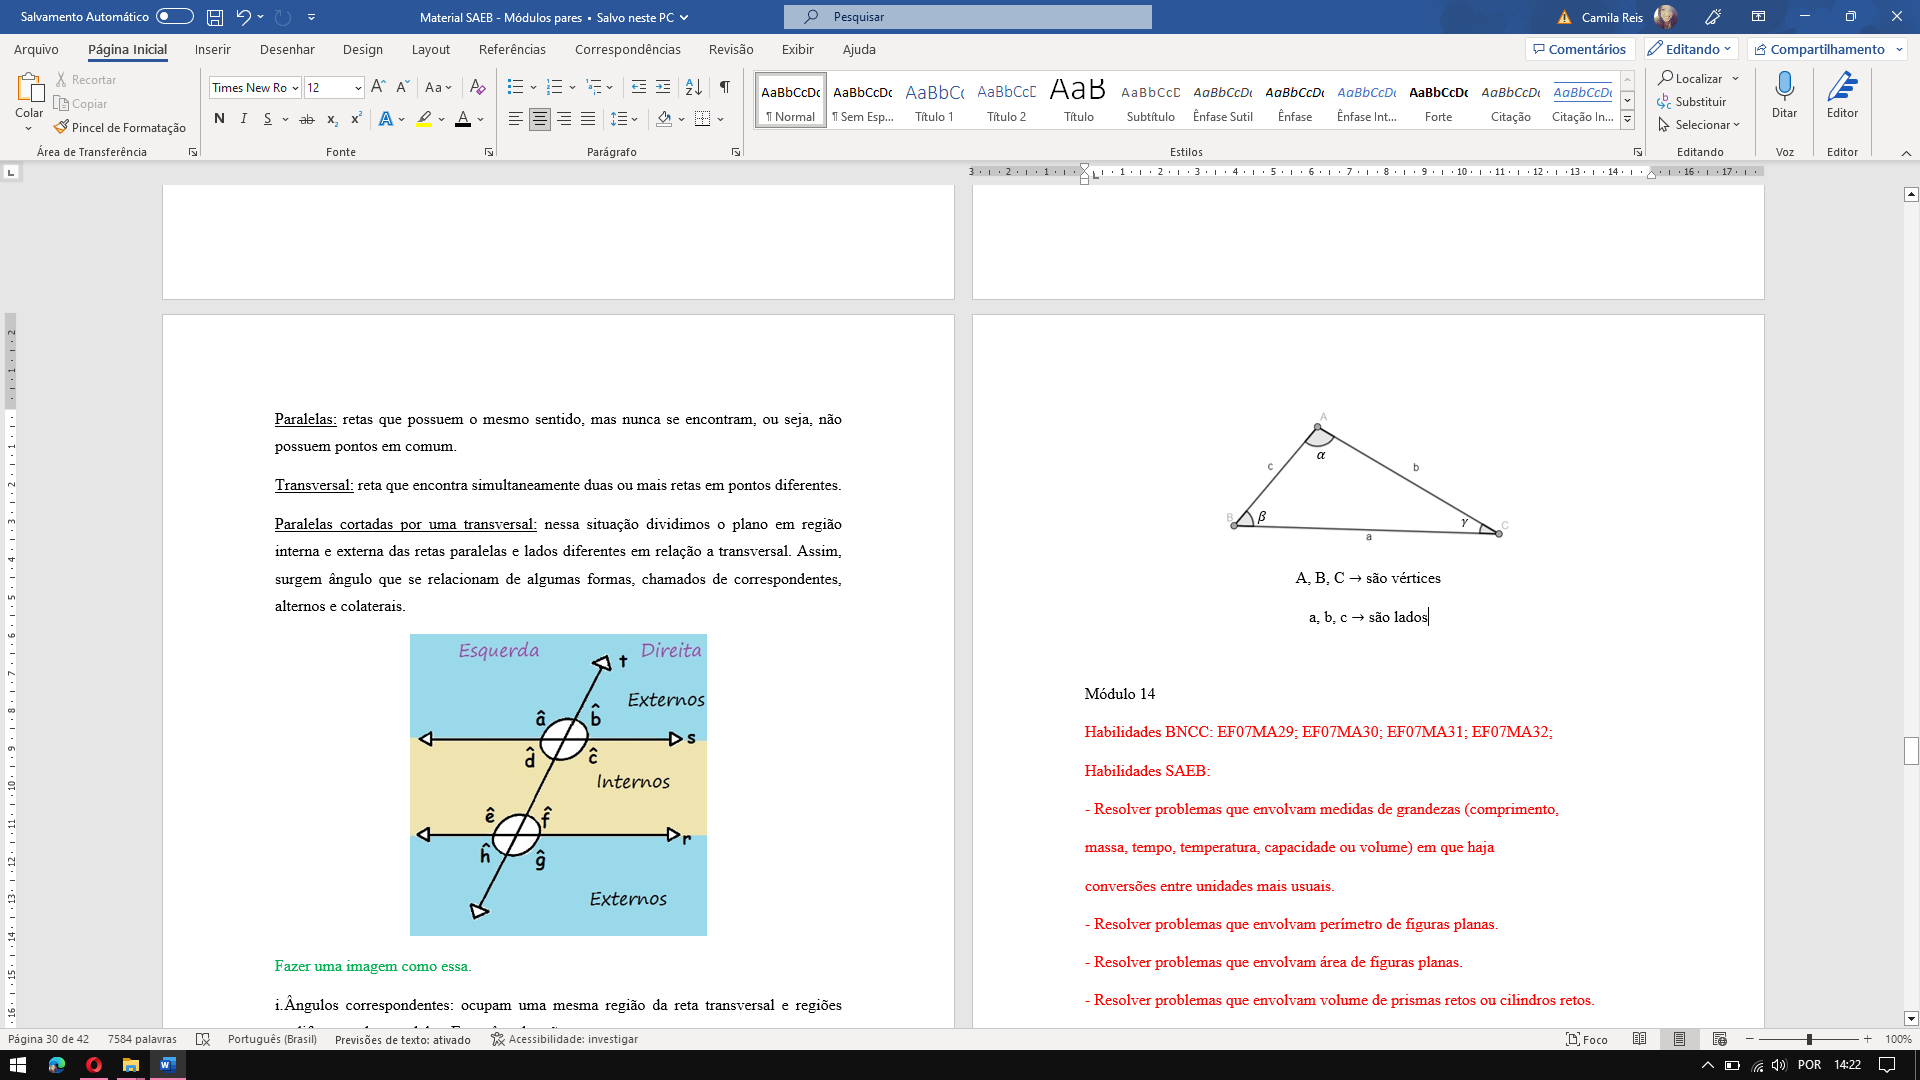
\includegraphics[width=5.15104in,height=3.10603in]{media/image41.png}

\begin{quote}
O Maracatu Nação apresenta um conjunto musical percussivo a um cortejo
real, evocando as coroações de reis e rainhas do antigo Congo africano.
Para o Iphan, o valor patrimonial do Maracatu Nação reside sua
capacidade de comunicar elementos da cultura brasileira e carregar
elementos essenciais para a memória, a identidade e a formação da
população afrobrasileira.

\fonte{Disponível em:
\emph{http://portal.iphan.gov.br/pagina/detalhes/504/}
Acesso em: 23 fev. 2023.}
\end{quote}

O Maracatu Nação é considerado um Patrimônio Histórico Imaterial de
nosso país. Para ser considerado Patrimônio Histórico Imaterial como o
Maracatu, uma prática, um objeto, ou um saber deve:

\begin{escolha}
\item render dinheiro à comunidade local.

\item representar a cultura de um grupo.

\item ser praticado dentro da família.

\item ter sido criado na atualidade.
\end{escolha}

\coment{BNCC: EF05HI10: Inventariar os patrimônios materiais e imateriais da
humanidade e analisar mudanças e permanências desses patrimônios ao
longo do tempo.

SAEB: 3B1. Compreender os significados culturais ou políticos de eventos
festivos de caráter histórico ou religioso.

a) Incorreto. A prática não deve necessariamente ter retorno financeiro
para ser considerada patrimônio;
b) Correto. Como o maracatu representa um aspecto da cultura
afro-brasileira, para ser nomeado Patrimônio Imaterial o proponente deve
também representar a cultura de seu grupo;
c) Incorreto. A prática não precisa ser necessariamente dentro da
família, mas pode ser de um grupo maior de pessoas;
d) Incorreto. Existem práticas muito antigas que podem ser consideradas
Patrimônio Imaterial e devem ser preservadas.}

\num{4} O parecer CNE/CP nº 03/2004 e a Resolução CNE/CP nº 01/2004 instituem a
obrigatoriedade do ensino de História e Cultura Afro-brasileira e
Africana nos currículos das escolas públicas e privadas da Educação
Básica. Essa modalidade legitimou-se pelo processo histórico de luta e
resistência dos povos negros e quilombolas, seus valores civilizatórios
afro-brasileiros e a política de pertencimento étnico, político e
cultural.

\fonte{Disponível em:
\emph{https://www.seduc.ce.gov.br/educacao-escolar-quilombola/}
Acesso em: 23 fev. 2023.}

Quilombolas são povos que vivem até hoje em comunidades de
afro-descendentes que combatiam a escravidão no país. Segundo o texto, a
obrigatoriedade do ensino de História e Cultura Afro-brasileira e
Africana nos currículos das escolas é importante para

\begin{escolha}
\item melhorar a qualidade das merendas escolares.

\item instituir a diversidade no ensino da cultura.

\item proteger as crianças em situação de rua.

\item garantir o fim da escravidão no Brasil.
\end{escolha}

\coment{Habilidade BNCC EF05HI04: Associar a noção de cidadania com os
princípios de respeito à diversidade, à pluralidade e aos direitos
humanos.

Habilidade SAEB: 5C1. Avaliar alternativas de ação em defesa de
diferentes expressões do patrimônio artístico e cultural brasileiro.

a) Incorreta. O ensino de história da África não garante a melhoria das
merendas na escola;
b) Correta. A obrigatoriedade do ensino de história da África contribui
para a diversidade do ensino da cultura de múltiplas etnias e raças no
Brasil;
c) Incorreta. Não há impacto sobre as crianças em situação de rua;
d) Incorreta. Já foi instituído o fim da escravidão no Brasil, o impacto
é na memória sobre este fenômeno.}

\num{5} O Home Office, ao pé da letra, significa escritório em casa. Ou seja, o
funcionário desenvolve as atividades em sua própria casa, sem ser
necessário o deslocamento até a empresa, realizando o trabalho em casa
utilizando principalmente da internet para se comunicar com seus chefes.

\fonte{Disponível em:
\emph{https://www.guiadacarreira.com.br/blog/5-vantagens-de-trabalhar-em-home-office}
Acesso em: 25 fev. 2023.}

Segundo o texto, hoje em dia trabalhar de casa só é possível por causa
da (do)

\begin{escolha}
\item desenvolvimento das tecnologias de comunicação.

\item aumento de empregos nas indústrias de produção.

\item dificuldade de encontrar empregos presenciais.

\item criação de novas tarefas de cuidado da casa.
\end{escolha}

\coment{Habilidade BNCC EF05GE05: Identificar e comparar as mudanças dos tipos
de trabalho e desenvolvimento tecnológico na agropecuária, na indústria,
no comércio e nos serviços.

Habilidade SAEB: 7A13. Identificar o uso de tecnologias na vida
doméstica, nos ambientes de lazer e do trabalho.

a) Correta. Trabalhar em casa só é possível porque o trabalhador
consegue se comunicar com seus colegas pela tecnologia;
b) Incorreta. O aumento de empregos em indústrias de produção não
influencia sobre o home office;
c) Incorreta. Não é mencionada uma dificuldade em encontrar empregos
presenciais;
d) Incorreta. Não é mencionada a criação de novas tarefas domésticas.}

\chapter{Simulado 2 }

\num{1} A Cetesb iniciou nesta quinta-feira, dia 16/04, a operação da nova
estação de monitoramento da qualidade do ar, instalada na escola de
educação infantil Prof. Zeferino Vaz, em Campinas. A unidade foi
adquirida com recursos de compensação ambiental do Aeroporto
Internacional de Viracopos, em função das obras de ampliação. A estação
vai avaliar a qualidade do ar da cidade, levando em consideração os
possíveis impactos de Viracopos, das rodovias Anhanguera, Bandeirantes e
Santos Dumont, bem como o conhecimento dos processos de transporte de
poluentes oriundos de outras regiões.

\fonte{Disponível em:
\emph{https://www.infraestruturameioambiente.sp.gov.br/2015/04/cetesb-inicia-hoje-operacao-da-nova-estacao-de-monitoramento-do-ar-de-campinas/}
Acesso em: 23 fev. 2023.}

A medida da prefeitura do município de Campinas, em São Paulo, é
importante para

\begin{escolha}
\item entender o impacto dos transportes na cidade.

\item diminuir a circulação de produtos na região.

\item avaliar os resultados de políticas ambientais.

\item melhorar a qualidade da educação nas escolas.
\end{escolha}

\coment{EF05GE12: Identificar órgãos do poder público e canais de participação
social responsáveis por buscar soluções para a melhoria da qualidade de
vida (em áreas como meio ambiente, mobilidade, moradia e direito à
cidade) e discutir as propostas implementadas por esses órgãos que
afetam a comunidade em que vive.

Habilidade SAEB 2C1: Julgar as vantagens ou os riscos da intervenção
humana na natureza.

a) Correta. A medida é importante para avaliar o impacto dos transportes
no ar e no meio ambiente do município;
b) Incorreta. Não há um interesse de diminuição da circulação de
produtos na região;
c) Incorreta. Não existe uma política ambiental sendo avaliada, mas sim
um impacto do uso de transportes;
d) Incorreta. Não há impactos sobre a qualidade da educação nas escolas.}

\num{2}

%
\includegraphics[width=6.26772in,height=4.55556in]{media/image42.png}

%Para o ilustrador: produzir um mapa do Brasil dividido pelas 5 regiões(1 - Norte, 5 - Nordeste, 3 - Centro-Oeste, 4 - Sudeste e 2 - Sul) e numerar dentro de cada região com o número indicado anteriormente.

O Brasil é dividido em cinco regiões. Identifique cada uma conforme sua
numeração no mapa:

\begin{escolha}
\item 1 - Nordeste, 2 - Centro-Oeste, 3 - Sudeste, 4 - Sul, 5 - Norte.

\item 1 - Norte, 2 - Centro-Oeste, 3 - Sul, 4 - Sudeste, 5 - Nordeste.

\item 1 - Nordeste, 2 - Sul, 3 - Norte, 4 - Centro-Oeste, 5 - Sudeste.

\item 1 - Norte, 2 - Sul, 3 - Centro-Oeste, 4 Sudeste, 5 - Nordeste.
\end{escolha}

\coment{Habilidade BNCC EF05HI02: Identificar os mecanismos de organização do
poder político com vistas à compreensão da ideia de Estado e/ou de
outras formas de ordenação social.

Habilidade SAEB 4A4:Identificar os espaços que compõem a estrutura
político-territorial do Brasil cartograficamente representados.

A alternativa correta é a d), cuja ordem corresponde às regiões.}

\num{3}

\begin{quote}
Entre 2003 e 2013 diversas cidades brasileiras viram protestos sobre a
gratuidade do transporte coletivo. Em 2013 o aumento da passagem em São
Paulo levou milhares de manifestantes às ruas. O Movimento Passe Livre
foi um dos grupos responsáveis pela divulgação e pela extensão que os
protestos ganharam. Atualmente no Brasil, diversas cidades adotam algum
tipo de isenção ou redução da tarifa principalmente para idosos,
deficientes ou estudantes. Algumas até aderiram à gratuidade integral,
sendo Volta Redonda (RJ), com 257.803 habitantes, e Maricá (RJ) 143.111
habitantes, as representantes mais populosas.

\fonte{Disponível em:
\emph{https://summitmobilidade.estadao.com.br/compartilhando-o-caminho/passe-livre-conheca-a-historia-do-movimento/}
Acesso em: 23 fev. 2023.}
\end{quote}

O Movimento Passe Livre, segundo o trecho, reivindicava

\begin{escolha}
\item ajudas do governo na compra de carros particulares.

\item melhorias das condições de trabalho dos motoristas.

\item utilização do transporte público de maneira gratuita.

\item reformas dos asfaltos das grandes metrópoles do país.
\end{escolha}

\coment{Habilidade BNCC EF05HI05: Associar o conceito de cidadania à conquista
de direitos dos povos e das sociedades, compreendendo-o como conquista
histórica.

Habilidade SAEB: 5B7. Relacionar a conquista de direitos à construção do
conceito ou ao exercício da cidadania.

a) Incorreta. O texto fala sobre transporte público e não particular;
b) Incorreta. O texto não fala sobre as condições dos motoristas;
c) Correta. O texto mostra que o movimento queria a gratuidade do
transporte público;
d) Incorreta. O texto não fala sobre a qualidade das vias.}

\num{4}

\begin{quote}
Campo Grande é a região do Rio que, historicamente, apresenta o maior
potencial de crescimento. Esse fato acontece por diversas razões. Por
estar situado nos limites do município, o bairro, de acordo com
especialistas, foi favorecido desde o nascimento da cidade por estradas
que atravessaram sua planície. Somam-se a isso seus abundantes
mananciais de água, a fertilidade de suas terras e, principalmente, a
chegada de pessoas com vocação empreendedora. Atualmente, a atividade
econômica local é composta por cerca de 3.700 estabelecimentos, 87,2\%
dos quais são do segmento de comércio e serviços, empregando
aproximadamente 49 mil pessoas. O volume de negócios gera R\$ 956,9
milhões de ICMS -- sexta arrecadação do município.
\end{quote}

Segundo o texto, o bairro Campo Grande no Rio de Janeiro tem potencial
de crescimento por causa de sua

\begin{escolha}
\item boa localização e interesse econômico.

\item qualidade educacional e beleza natural.

\item atração turística e importância histórica.

\item riqueza mineral e produção gastronômica.
\end{escolha}

\coment{Habilidades da BNCC envolvidas: EF05HI0: Identificar os processos de
formação das culturas e dos povos, relacionando-os com o espaço
geográfico ocupado.

SAEB: 1C5. Explicar características, semelhanças e diferenças das
mudanças temporais e/ou espaciais.

a) Correta. O texto fala sobre sua boa localização - limites do
município - e sobre o interesse de empresários em seu potencial de
crescimento;
b) Incorreta. Não há menção à educação nem à beleza da paisagem;
c) Incorreta. Não há menção ao turismo ou ao passado do bairro;
d) Incorreta. Não há menção a riquezas minerais nem a um polo
gastronômico.}

\num{5}

\begin{quote}
\textbf{Ingredientes para receita de Hambúrguer:}\\
200 gramas de carne moída\\
1 tomate\\
100 gramas de alface\\
1 cebola\\
1 pão
\end{quote}

De quais setores de trabalho precisamos para conseguir os ingredientes
para preparar uma receita de hambúrguer em casa?

\begin{escolha}
\item agricultura e pecuária.

\item agricultura e turismo.

\item pecuária e mineração.

\item pecuária e turismo.
\end{escolha}

\coment{BNCC EF05GE05: Identificar e comparar as mudanças dos tipos de trabalho
e desenvolvimento tecnológico na agropecuária, na indústria, no comércio
e nos serviços.

SAEB 7B7: Analisar a interdependência econômica entre campo e cidade.

a) Correta. Precisamos da pecuária para as carnes e da agricultura para
os demais ingredientes;
b) Incorreta. Não precisamos do turismo;
c) Incorreta. Não precisamos da mineração;
d) Incorreta. Não precisamos do turismo.}

\chapter{Simulado 3}

\num{1} Os objetos biográficos dão significado à casa da família de Hugo e
estão guardados em seu interior, sendo que a presença deles neste lugar
dá a sensação de continuidade da vida do próprio Hugo. Embora esteja
praticamente abandonada um dia foi habitada e nela os objetos ainda
existentes reportam a pertença a alguém que os usou no cotidiano. Como
cita Malvina Muszkat ``o sentimento de continuidade se relaciona à
dimensão tempo, no sentido de se manter único através de diferentes
tempos e de ser `conscientizado' através do exercício da memória''.

\fonte{GOMES, COSTA. A Casa e os objetos de memória. \textbf{Revista Iniciação
Científica}, Criciúma, v. 14, n. 1, 2016}

Segundo o texto, os objetos da casa de Hugo podem ser considerados

\begin{escolha}
\item ameaças ao meio ambiente.

\item lixos a serem reciclados.

\item documentos históricos.

\item bens muito caros.
\end{escolha}

\coment{EF05HI07: Identificar os processos de produção, hierarquização e difusão
dos marcos de memória e discutir a presença e/ou a ausência de
diferentes grupos que compõem a sociedade na nomeação desses marcos de
memória.

SAEB: 1B2: Compreender a função, o uso e o significado de objetos e
documentos pessoais.

a) Incorreta. O texto não fala que os objetos ameaçam o meio ambiente;
b) Incorreta. O texto não trata como lixo, mas como objeto de memória;
c) Correta. Os objetos são tratados como objetos de memória, ou seja,
documentos sobre a história de Hugo;
d) Incorreta. Não é falado sobre o valor material dos objetos.}

\num{2}

%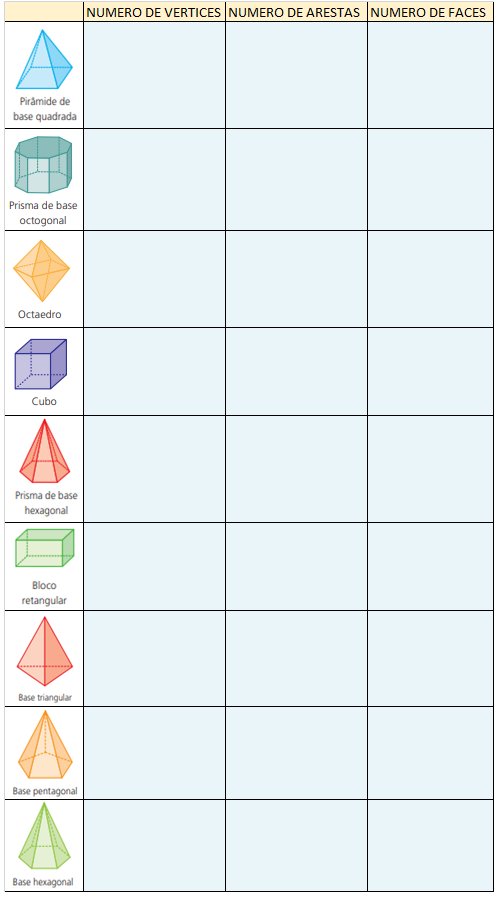
\includegraphics[width=5.60938in,height=4.48191in]{media/image43.png}
%\fonte{Disponível em: \emph{https://br.freepik.com/vetores-gratis/fundo-do-corredor-da-escola-suja\_4228059.htm\#query=escola\%20lixo\&position=0\&from\_view=search\&track=ais} Acesso em: 23 fev. 2023.}

A imagem acima representa a seguinte ação individual prejudicial ao meio
ambiente:

\begin{escolha}
\item cortar árvores em florestas.

\item realizar reciclagem de papéis.

\item queimar plantações nos campos.

\item jogar lixo em locais inadequados.
\end{escolha}

\coment{BNCC EF05GE11: Identificar e descrever problemas ambientais que ocorrem
no entorno da escola e da residência (lixões, indústrias poluentes,
destruição do patrimônio histórico etc.), propondo soluções (inclusive
tecnológicas) para esses problemas.

SAEB:2B9. Identificar atividades humanas potencialmente causadoras de
impactos ambientais.

a) Incorreta. A imagem não mostra o corte de árvores;
b) Incorreta. A imagem não mostra reciclagem de papéis, além dela ser
benéfica ao meio ambiente;
c) Incorreta. A imagem não mostra campos queimados;
d) Correta. A imagem mostra lixos jogados no chão da escola, local
inadequado.}

\num{3}

\begin{quote}
Atribui-se aos gregos, na Antiguidade, a invenção das vogais, a
difusão e adoção do alfabeto da sociedade fenícia, como também a
invenção do método de alfabetização sobre o qual podemos afirmar que
milhões de pessoas aprenderam a ler e a escrever, através dos três
milhares de anos que se passaram desde que as primeiras crianças
``cantaram'' o bê-a-bá. Este método, onde se aprendia separadamente a
ler e a escrever, foi sendo adotado por outros povos, passando por
adaptações e transformações, mas, em geral, chamado simplesmente de
alfabetização.

\fonte{STAMATTO, Maria. Alfabetização Histórica em materiais didáticos:
significados e usos \textbf{ANPUH} -- XXV SIMPÓSIO NACIONAL DE HISTÓRIA
-- Fortaleza, 2009.}
\end{quote}

Segundo o texto, uma importante invenção dos fenícios para nossa sociedade foi:

\begin{escolha}
\item a escrita.

\item a escola.

\item o alfabeto.

\item o livro.
\end{escolha}

\coment{BNCC EF05HI03: Analisar o papel das culturas e das religiões na
composição identitária dos povos antigos.

SAEB: 3A11. Identificar evidências da contribuição cultural de grupos de
diferentes origens étnicas.

a) Incorreta. A escrita não foi inventada pelos fenícios;
b) Incorreta. A escola não foi inventada pelos fenícios;
c) Correta. O texto fala sobre a utilização pelos gregos do alfabeto
criado pelos fenícios;
d) Incorreta. Não foram os fenícios que criaram o livro.}

\num{4}

\begin{quote}
Em geral, a base da organização social de um povo indígena é a
família extensa, entendida como uma unidade social articulada em torno
de um patriarca ou de uma matriarca por meio de relações de parentesco
ou afinidade política ou econômica. São denominadas famílias extensas
por aglutinarem um número de pessoas e de famílias muito maior que uma
família tradicional européia. Uma família extensa indígena geralmente
reúne a família do patriarca ou da matriarca, as famílias dos filhos,
dos genros, das noras, dos cunhados e outras famílias afins que se
filiam à grande família por interesses específicos.

\fonte{DOS SANTOS, Luciano(Baniwa). \textbf{O índio brasileiro.} Secretaria de
Educação Continuada, Alfabetização e Diversidade (Secad), Organização
das Nações Unidas para a Educação, a Ciência e a Cultura (Unesco) e
Projeto Trilhas de Conhecimentos -- LACED/Museu Nacional, 2006.}
\end{quote}

Segundo o texto, a família extensa é, para os indígenas,

\begin{escolha}
\item uma organização proibida nas aldeias.

\item uma lenda contada pelos mais velhos.

\item uma junção de vários grupos familiares.

\item um outro nome para se chamar o povo nativo.
\end{escolha}

\coment{EF05HI02: Identificar os mecanismos de organização do poder político com
vistas à compreensão da ideia de Estado e/ou de outras formas de
ordenação social.

SAEB: 4B4. Compreender as mudanças e permanências nas formas de
organização familiar em diferentes sociedades contemporâneas.

a) Incorreta. Não é uma organização proibida, mas sim a base da
sociedade;
b) Incorreta. Não é uma lenda, mas a organização principal das aldeias;
c) Correta. É uma junção de vários grupos familiares por diversos
interesses;
d) Incorreta. Não pode ser utilizada para denominar os povos nativos.}

\num{5}

\begin{quote}
\textbf{Campanha pela Valorização do Trabalho Doméstico}

Queremos trazer para pauta das discussões da sociedade a questão do
trabalho doméstico remunerado com o objetivo de sensibilizar a sociedade
civil e os agentes públicos para o reconhecimento dos direitos das
trabalhadoras domésticas, pela igualdade de direitos com as demais
categorias. São consideradas trabalhadoras domésticas as pessoas maiores
de 18 anos que prestam serviço de natureza contínua (com frequência) e
de finalidade não lucrativa à pessoa ou à família, no espaço residencial
destas.

\fonte{Disponível em:
\emph{https://centrac.org.br/publicacoes/campanhas/campanha-pela-valorizacao-do-trabalho-domestico/}
Acesso em: 23 fev. 2023.}
\end{quote}

Um exemplo de trabalhadora doméstica e sua importância é:

\begin{escolha}
\item secretária, que organiza as coisas dentro de um escritório.

\item padeira, que produz os pães a serem vendidos na padaria.

\item vendedora, que mostra os produtos disponíveis na loja.

\item faxineira, que mantém a limpeza do ambiente da casa.
\end{escolha}

\coment{EF05GE05: Identificar e comparar as mudanças dos tipos de trabalho e
desenvolvimento tecnológico na agropecuária, na indústria, no comércio e
nos serviços.

SAEB: 7C9: Avaliar a importância das diversas formas de trabalho
existentes, propondo estratégias para sua valorização.

a) Incorreta. A secretária não trabalha no ambiente doméstico;
b) Incorreta. A padeira não trabalha no ambiente doméstico, mas na
padaria;
c) Incorreta. A vendedora trabalha na loja e não na casa;
d) Correta. A faxineira é uma trabalhadora doméstica responsável pela
limpeza da casa.}

\chapter{Simulado 4}

\num{1}

%
\includegraphics[width=3.84896in,height=3.84256in]{media/image44.png}
%Disponível em: \emph{https://br.freepik.com/vetores-gratis/mao-com-calendario-de-marca-de-caneta\_1250622.htm\#query=calend\%C3\%A1rio\&position=18\&from\_view=search\&track=sph} Acesso em: 23 fev. 2023.

A imagem acima representa o seguinte marcador temporal:

\begin{escolha}
\item o relógio.

\item a ampulheta.

\item o diário.

\item o calendário
\end{escolha}

\coment{BNCC EF05HI07: Identificar os processos de produção, hierarquização e
difusão dos marcos de memória e discutir a presença e/ou a ausência de
diferentes grupos que compõem a sociedade na nomeação desses marcos de
memória.

SAEB: 1A3. Identificar diferentes marcadores do tempo, como o relógio e
o calendário.

a) Incorreta. Não é um relógio;
b) Incorreta. Não é uma ampulheta;
c) Incorreta. Não é um diário;
d) Correta. É um calendário.}

\num{2}

\begin{quote}
\textbf{Expansão urbana global ameaça 205 espécies de animais, diz estudo.}

Até 2030, novas cidades do planeta ocuparão 1,2 milhão de km² de área.
Mata Atlântica, Cerrado e outros biomas do mundo podem ser degradados.
Um novo estudo realizado por pesquisadores norte-americanos afirma que
até 2030, 1,2 milhão de km² do planeta deixarão de ser áreas preservadas
para dar lugar a grandes cidades -- uma área equivalente ao dobro do
tamanho do estado da Bahia. A partir da análise, os especialistas
afirmam que é preciso desenvolver projetos sustentáveis para os próximos
28 anos, o que evitaria um grande impacto ao meio ambiente e às futuras
gerações humanas.
\end{quote}

Segundo o texto, a expansão urbana global ameaça os animais pois o
aumento das cidades

\begin{escolha}
\item diminui a área de plantações de alimento.

\item melhora a condição de vida dos humanos.

\item invade os territórios onde eles habitam.

\item baixa a destruição das florestas.
\end{escolha}

\coment{Habilidade BNCC EF05GE03: Identificar as formas e funções das cidades e
analisar as mudanças sociais, econômicas e ambientais provocadas pelo
seu crescimento.

SAEB: 2A3. Identificar as características das paisagens naturais ou
antrópicas.

a) Incorreta. O texto não fala sobre a ocupação de áreas agrícolas, mas
de biomas preservados;
b) Incorreta. O texto não fala que a melhora na vida dos humanos piora a
vida animal;
c) Correta. A expansão urbana invade biomas e áreas preservadas e
destinadas à vida animal;
d) Incorreta. O aumento das cidades não baixa a destruição das
florestas, pelo contrário, aumenta.}

\num{3}

\begin{quote}
Por que as religiões de matriz africana são o principal alvo de
intolerância religiosa no Brasil?

Por um lado o racismo e a discriminação que remontam à escravidão e que
desde o Brasil colônia rotulam tais religiões pelo simples fato de serem
de origem africana, e, pelo outro, a ação de movimentos neopentecostais
que nos últimos anos teriam se valido de mitos e preconceitos para
``demonizar'' e estimular a perseguição a umbandistas e candomblecistas.
Os dados do Disque 100, criado pela Secretaria Nacional de Direitos
Humanos, apontam 697 casos de intolerância religiosa entre 2011 e
dezembro de 2015.
\end{quote}

Segundo o texto, um dos motivos da discriminação contra as religiões
citadas no texto é

\begin{escolha}
\item a falta de denúncias contra crimes de intolerância.

\item a diversidade cultural ensinada nas escolas públicas.

\item a violência de grupos descendentes de ex-escravos.

\item o preconceito com a comunidade afro-brasileira.
\end{escolha}

\coment{BNCC EF05GE02: Identificar diferenças étnico-raciais e étnico-culturais
e desigualdades sociais entre grupos em diferentes territórios.

SAEB 3C3: Avaliar a presença e/ou a ausência de representação de
diferentes grupos sociais na construção de marcos de memória.

a) Incorreta. O texto mostra que existem muitas denúncias;
b) Incorreta. A diversidade ensinada nas escolas melhoraria o problema,
não seria o motivo dele;
c) Incorreta. O texto não fala que essas comunidades são violentas, mas
sim violentadas;
d) Correta. O texto fala que ainda há resquícios de racismo em nossa
sociedade.}

\num{4}

\begin{quote}
O Instituto do Patrimônio Histórico e Artístico Nacional (Iphan)
(...) responde pela preservação do Patrimônio Cultural Brasileiro. Cabe
ao Iphan proteger e promover os bens culturais do País, assegurando sua
permanência e usufruto para as gerações presentes e futuras.
\end{quote}

Um exemplo de local que pode ser protegido pelo IPHAN é:

\begin{escolha}
\item um condomínio de casas.

\item uma plantação de arroz.

\item uma igreja muito antiga.

\item uma floresta no litoral.
\end{escolha}

\coment{BNCC EF05HI02: Identificar os mecanismos de organização do poder
político com vistas à compreensão da ideia de Estado e/ou de outras
formas de ordenação social.

4C2: Discutir os elementos políticos e sociais ligados às políticas de
reconhecimento e gestão do patrimônio.

a) Incorreta. Um condomínio residencial não é considerado patrimônio
histórico e artístico pelo IPHAN;
b) Incorreta. Uma plantação de arroz não é considerada patrimônio
histórico e artístico pelo IPHAN;
c) Correta. Uma igreja muito antiga pode fazer parte do patrimônio
protegido pelo IPHAN;
d) Incorreta. Uma floresta não é considerada patrimônio histórico e
artístico pelo IPHAN mas sim patrimônio da natureza.}

\num{5}

\begin{quote}
\textbf{Copa do Mundo: entenda as denúncias sobre direitos humanos contra o Catar }

Desde que foi escolhido como sede da Copa, em 2010, país sofre críticas
sobre tratamento das mulheres, membros da comunidade LGBT, trabalhadores
migrantes e jornalistas, por exemplo. As mulheres no Catar (...)
enfrentam discriminação generalizada tanto na lei quanto na prática.
Pelas denúncias que envolvem os direitos humanos, a seleção da Dinamarca
pretendia usar camisetas durantes seus treinos na Copa do Mundo com
mensagem em prol dos direitos humanos.

\fonte{Disponível em:
\emph{https://www.cnnbrasil.com.br/esporte/copa-do-mundo-entenda-as-denuncias-sobre-direitos-humanos-contra-o-catar/}
Acesso em: 23 fev. 2023.}
\end{quote}

Segundo a reportagem, o direito humano que não estaria sendo seguido
pelo governo do Catar é:

\begin{escolha}
\item direito de proteção à tortura.

\item direito à moradia.

\item direito à nacionalidade.

\item direito à igualdade.
\end{escolha}

\coment{BNCC EF05HI04: Associar a noção de cidadania com os princípios de
respeito à diversidade, à pluralidade e aos direitos humanos.

SAEB 5A3: Reconhecer formas de atuação condizentes e não condizentes com
os direitos humanos nos espaços público e doméstico.

a) Incorreta. O texto não fala sobre o ferimento do direito de proteção
à tortura;
b) Incorreta. O texto não fala que as pessoas não tem direito à moradia;
c) Incorreta. O texto não fala que existem pessoas sem nacionalidade no
Catar;
d) Correta. O texto fala que as mulheres são discriminadas, e que certas
comunidades não tem direitos iguais a outras.}


